% ================================================================
% CHAPTERS 15--22: ADVANCED THEORY OF IDEATIC DIFFUSION
% ================================================================
% This file contains no preamble. It is \input'd by idt_book_v2.tex.


% ================================================================
% CHAPTER 15: COOPERATION AND COALITION THEORY
% ================================================================
\chapter{Cooperation and Coalition Theory}
\label{ch:coalitions}

\epigraph{No man is an island, entire of itself; every man is a piece of the
continent, a part of the main.}{John Donne, \textit{Devotions upon Emergent
Occasions}}

\section{From Pairs to Coalitions}

In earlier chapters we studied interaction between \emph{pairs} of ideas.  The
angle $\cosangle{a}{b}$ classified each dyadic encounter as cooperative,
competitive, or orthogonal (Chapter~\ref{ch:cooperation}).  But cultural life
is not dyadic: ideas combine in coalitions, organizations adopt bundles of
practices, and the value of any single idea depends on the ideas it is combined
with.  This chapter extends the pairwise theory to \emph{coalitions} ---
arbitrary finite sets of ideas that are composed together.

\begin{definition}[Coalition]
\label{def:coalition}
A \textbf{coalition} is a finite, non-empty subset $S \subseteq \IS$.  The
\textbf{coalition composition} is the iterated composition:
\[
  \bigcompose S := a_1 \compose a_2 \compose \cdots \compose a_k,
\]
where $S = \{a_1, \ldots, a_k\}$.  By the associativity guaranteed by the
Hilbert-space embedding (Section~\ref{sec:composition}), the result is
independent of the ordering.
\end{definition}

\begin{remark}
Strictly, the composition $\compose$ in IDT need not be commutative, so
$\bigcompose S$ depends on the ordering unless the ideas pairwise commute under
composition.  When we write $\bigcompose S$ without specifying an order, we
assume either that commutativity holds or that a canonical ordering has been
fixed.
\end{remark}

\begin{interpretation}
\label{interp:ch15:bakhtin_great_dialogue}
The concept of a coalition formalizes what Mikhail Bakhtin called the ``great dialogue'' --- the ceaseless
interplay of voices that constitutes cultural life.  For Bakhtin, no utterance
exists in isolation; every word is ``half someone else's,'' acquiring meaning
only through its interaction with other words, other speakers, other
ideological horizons.  The coalition $S = \{a_1, \ldots, a_k\}$ is the
mathematical counterpart of this polyphonic ensemble.  Each idea $a_i$ is a
``voice'' in the Bakhtinian sense, and the coalition composition
$\bigcompose S$ is the composite utterance that emerges from their
interaction.

What IDT adds to Bakhtin's insight is \emph{precision}: the composition
operator $\compose$ and the Hilbert-space embedding $\varphi$ transform
the metaphor of ``dialogue'' into a geometric object whose properties can be
proved.  Where Bakhtin speaks evocatively of ``heteroglossia'' and
``polyphony,'' IDT provides a calculus: we can measure the synergy of
voices (the cooperation surplus $\sigma$), prove that the ensemble is
richer than any sub-ensemble (enrichment), and compute the fair attribution
of value to each voice (the Shapley value of Chapter~\ref{ch:shapley}).
The result is not a reduction of Bakhtin's literary vision to mathematics,
but an \emph{amplification}: the formalism reveals structural features of
dialogic interaction --- the cocycle condition, the spectral decomposition
of emergence --- that Bakhtin's qualitative framework could not articulate.
\end{interpretation}

\subsection{Coalition Value}

The central question of coalition theory is: \emph{how much is a coalition
worth?}  In classical cooperative game theory, the value function
$v\colon 2^N \to \mathbb{R}$ assigns a real number to every subset of
players.  We define the analogous concept for ideas.

\begin{definition}[Coalition Value]
\label{def:coalition-value}
The \textbf{coalition value} of a finite set $S \subseteq \IS$ is the
self-resonance of its composition:
\[
  v(S) := \rs{\bigcompose S}{\bigcompose S} = \nrm{\embed{\bigcompose S}}^2.
\]
\end{definition}

The coalition value measures the \emph{total ideatic energy} of the composite
idea.  The enrichment axiom (Axiom~\ref{ax:enrichment}) ensures that adding
ideas to a coalition never decreases its value, a property that connects
directly to the theory of superadditive games.

\begin{theorem}[Enrichment Implies Superadditivity]
\label{thm:enrichment-superadditive}
For any idea $a \in \IS$ and any coalition $S$ with $a \notin S$:
\[
  v(S \cup \{a\}) \geq v(S).
\]
Hence the coalition value function $v$ is \textbf{monotone}: larger coalitions
are worth at least as much as smaller ones.
\end{theorem}

\begin{proof}
Let $c = \bigcompose S$.  Then $\bigcompose (S \cup \{a\}) = a \compose c$
(up to ordering).  By the enrichment axiom,
\[
  \rs{a \compose c}{a \compose c} \geq \rs{c}{c},
\]
which is exactly $v(S \cup \{a\}) \geq v(S)$.
\end{proof}

\begin{interpretation}
Monotonicity of coalition value is a formalization of the intuition that
``more ideas, more meaning.''  A culture that absorbs a new practice,
technology, or concept never loses total ideatic content --- at worst the new
idea is orthogonal and adds nothing, at best it creates synergistic resonance.
The asymmetry is striking: ideas can enrich but never impoverish a coalition.
This is \emph{not} true in general economic models, where adding a player can
destroy value through coordination failures.  In IDT, the embedding in Hilbert
space geometrically prevents such destruction.
\end{interpretation}

\begin{interpretation}
\label{interp:ch15:kristeva_intertextuality}
Julia Kristeva's theory of intertextuality --- the principle that ``any text is
the absorption and transformation of another'' --- receives here its
mathematical vindication.  Kristeva, developing Bakhtin's dialogism for the
structuralist era, argued that texts do not merely \emph{refer to} one another
but are constituted by their intertextual relations: a text is a ``mosaic of
quotations,'' a coalition of absorbed and transformed prior texts.

Theorem~\ref{thm:enrichment-superadditive} formalizes the most radical
implication of Kristeva's claim.  If each ``text'' is an idea $a_i$ and the
literary tradition is the coalition $S$, then the absorption of a new text
into the tradition ($S \cup \{a\}$) can never diminish the tradition's total
ideatic content.  This is precisely Kristeva's point: intertextuality is
\emph{constitutive}, not parasitic.  When T.\,S.\ Eliot absorbs Dante, the
result is not Eliot minus originality but Eliot-plus-Dante, a composite whose
self-resonance exceeds either component.  The enrichment axiom mathematically
guarantees what Kristeva argues textually: absorbing the other always enriches.

Yet the formalism also reveals a tension in Kristeva's framework.  If
intertextuality is always enriching (monotone), how do we account for the
common experience that some textual combinations are cacophonous or
incoherent?  The IDT answer lies in the distinction between self-resonance
(total ideatic energy, which is monotone) and cross-resonance with specific
probes (which can be negative).  A text may become richer in total content
through intertextual absorption while becoming \emph{less resonant} with
particular readers or interpretive communities.  This distinction, invisible
to Kristeva's qualitative framework, is precisely the kind of refinement that
formalization enables.
\end{interpretation}

\section{The Cooperation Surplus}

Knowing that coalitions are monotone is a start, but we want a finer measure
of the \emph{synergy} created when ideas combine.

\begin{definition}[Cooperation Surplus]
\label{def:cooperation-surplus}
The \textbf{cooperation surplus} of ideas $a$ and $b$ is:
\[
  \sigma(a, b) := v(\{a, b\}) - v(\{a\}) - v(\{b\})
  = \rs{a \compose b}{a \compose b} - \rs{a}{a} - \rs{b}{b}.
\]
More generally, for a coalition $S$ and a new idea $a$:
\[
  \sigma(a \mid S) := v(S \cup \{a\}) - v(S) - v(\{a\}).
\]
\end{definition}

\begin{interpretation}
\label{interp:ch15:grice_cooperation}
The cooperation surplus $\sigma(a,b)$ formalizes a concept at the very heart
of the philosophy of language: Paul Grice's \textbf{cooperative principle}.
Grice argued that conversation succeeds because participants cooperate ---
they follow maxims of quantity, quality, relation, and manner not because
they are logically compelled to but because cooperation generates
communicative surplus.  A conversation where participants merely
juxtapose their ideas (linear composition, $\sigma = 0$) communicates only
the sum of individual contributions.  But genuine Gricean cooperation
creates \emph{implicature} --- meaning that emerges from the interplay
of utterances and exceeds their literal content.

In IDT, implicature is precisely the cooperation surplus $\sigma(a,b)$.
When two conversational contributions resonate positively ($\rs{a}{b} > 0$),
their composition amplifies this resonance; when they resonate negatively
(irony, contradiction), the non-linear term $\Delta(a,b)$ can still generate
positive surplus through what Grice would call ``flouting'' a maxim ---
the deliberate violation that creates higher-order meaning.

Umberto Eco extended Grice's framework into a general theory of textual
cooperation.  In Eco's \textit{The Role of the Reader} (1979), the ``model
reader'' is not a passive recipient but an active cooperator who fills in
textual gaps, resolves ambiguities, and generates interpretive surplus.
The cooperation surplus $\sigma(a,b)$ quantifies exactly this: the excess
meaning that arises when reader (idea $a$) and text (idea $b$) combine
beyond what either contains independently.
\end{interpretation}

\begin{theorem}[Surplus Decomposition]
\label{thm:surplus-decomposition}
The cooperation surplus of $a$ and $b$ satisfies:
\[
  \sigma(a, b) = 2\,\rs{a}{b} + \Delta(a, b),
\]
where $\Delta(a, b) := \rs{a \compose b}{a \compose b} - \rs{a}{a} - \rs{b}{b}
- 2\,\rs{a}{b}$ captures higher-order interaction effects beyond pairwise
resonance.
\end{theorem}

\begin{proof}
This is immediate from the definition.  The key observation is that if the
embedding were perfectly linear (i.e., $\embed{a \compose b} = \embed{a} +
\embed{b}$), then:
\[
  \rs{a \compose b}{a \compose b} = \nrm{\embed{a} + \embed{b}}^2
  = \rs{a}{a} + 2\,\rs{a}{b} + \rs{b}{b},
\]
giving $\Delta(a, b) = 0$.  The term $\Delta(a, b)$ measures the departure
from linearity --- the genuinely \emph{emergent} contribution of composition.
\end{proof}

\begin{interpretation}
\label{interp:ch15:hegel_master_slave}
The surplus decomposition reveals a structure that resonates deeply with
Hegel's master-slave dialectic (\textit{Phenomenology of Spirit}, \S178--196).
Hegel describes how two self-consciousnesses, initially in opposition
($\rs{a}{b} < 0$, a ``life-and-death struggle''), arrive at a relationship
that generates a surplus of self-awareness neither possessed alone.  The
master gains recognition; the slave gains self-consciousness through labor.
The total ``ideatic content'' of the dyad exceeds the sum of the individuals.

In our decomposition, the term $2\rs{a}{b}$ captures the \emph{direct}
interaction --- for Hegel, the immediate encounter between master and slave.
When this is negative (opposition), direct interaction diminishes the sum.
But the term $\Delta(a,b)$ --- the non-linear surplus --- captures what Hegel
calls the \emph{productivity} of the encounter: the new forms of
consciousness that emerge from the dialectical struggle.  The master-slave
dialectic ``works'' (produces Aufhebung) precisely when $\Delta(a,b)$ is
large enough to overcome the negative $2\rs{a}{b}$.

This provides a quantitative criterion for when dialectical opposition is
\emph{productive} versus merely destructive: opposition generates positive
surplus if and only if the non-linear interaction term $\Delta(a,b) >
-2\rs{a}{b} = 2|\rs{a}{b}|$.  Hegel intuited that not all contradictions
are creative; IDT identifies the precise condition that separates
productive from sterile opposition.
\end{interpretation}

\begin{example}[Musical Harmony as Coalition]
Consider three notes $C, E, G$ forming a major triad.  Each note has
self-resonance $v(\{C\}) = v(\{E\}) = v(\{G\}) \approx 1$.  The pairwise
surplus $\sigma(C, E) > 0$ reflects the consonance of a major third.  But the
coalition value $v(\{C, E, G\})$ exceeds the sum of pairwise surpluses --- the
triad has an emergent harmonic richness that no pair captures.  This is
precisely the $\Delta$ term: the non-linear, higher-order contribution of the
composition.
\end{example}

\section{Ordered Coalition Enrichment}

In many cultural settings, the \emph{order} in which ideas are introduced
matters.  A technology adopted before the social institutions needed to regulate
it produces different outcomes than the reverse sequence.

\begin{definition}[Ordered Coalition]
\label{def:ordered-coalition}
An \textbf{ordered coalition} is a sequence $(a_1, a_2, \ldots, a_k)$ of
ideas.  Its value is computed by sequential composition:
\[
  v_{\mathrm{ord}}(a_1, \ldots, a_k) := \rs{a_1 \compose a_2 \compose \cdots
  \compose a_k}{a_1 \compose a_2 \compose \cdots \compose a_k}.
\]
\end{definition}

\begin{theorem}[Ordered Enrichment]
\label{thm:ordered-enrichment}
For any ordered coalition $(a_1, \ldots, a_k)$ and any idea $a_{k+1}$:
\[
  v_{\mathrm{ord}}(a_1, \ldots, a_k, a_{k+1}) \geq
  v_{\mathrm{ord}}(a_1, \ldots, a_k).
\]
\end{theorem}

\begin{proof}
Let $c = a_1 \compose \cdots \compose a_k$.  Then
$v_{\mathrm{ord}}(a_1, \ldots, a_k, a_{k+1}) = \rs{c \compose a_{k+1}}{c
\compose a_{k+1}} \geq \rs{c}{c} = v_{\mathrm{ord}}(a_1, \ldots, a_k)$
by the enrichment axiom.
\end{proof}

\begin{interpretation}
\label{interp:ch15:oulipo_collaboration}
Ordered coalition enrichment has a striking realization in the practice of
collaborative literary composition.  The Oulipo group --- founded by Raymond
Queneau and Fran\c{c}ois Le Lionnais in 1960 --- developed systematic
procedures for constrained collaborative writing: each author contributes
in sequence, and the composition is irrevocably enriched at each step.  The
Surrealist ``exquisite corpse'' game operates similarly: each participant
adds a word or phrase without seeing the others', and the result is an
ordered coalition whose value is guaranteed (by our theorem) to be at least
as great as any sub-sequence.

The ordered structure is essential here, not incidental.  A sentence
composed as ``noun-verb-adjective'' produces a different idea than
``adjective-noun-verb.''  The fact that ordered enrichment holds
\emph{regardless} of the order chosen (each order yields monotonic
enrichment) is a mathematical expression of what the Oulipo called
``potential literature'': every ordering of the same raw materials
produces a monotonically enriched composition, but different orderings
explore different regions of the ideatic space.  The literary game is
not to find the \emph{one} correct order but to recognize that every
order is an act of creation.
\end{interpretation}

\begin{lstlisting}
-- Lean 4: Ordered Coalition Enrichment
theorem ordered_coalition_enriches (rs : IS → IS → ℝ) (compose : IS → IS → IS)
    (enrichment : ∀ a b, rs (compose a b) (compose a b) ≥ rs a a)
    (coalition : List IS) (a : IS) :
    rs (coalition.foldl compose a) (coalition.foldl compose a) ≥ rs a a := by
  induction coalition with
  | nil => simp
  | cons x xs ih =>
    simp [List.foldl]
    calc rs (List.foldl compose (compose a x) xs)
           (List.foldl compose (compose a x) xs)
        ≥ rs (compose a x) (compose a x) := ih (compose a x)
      _ ≥ rs a a := enrichment a x
\end{lstlisting}

\section{Marginal Contribution and the Core}

\begin{definition}[Marginal Contribution]
\label{def:marginal-contribution}
The \textbf{marginal contribution} of idea $a$ to coalition $S$ (where
$a \notin S$) is:
\[
  \Delta_a(S) := v(S \cup \{a\}) - v(S).
\]
By enrichment (Theorem~\ref{thm:enrichment-superadditive}), $\Delta_a(S) \geq 0$
always.
\end{definition}

\begin{definition}[The Core]
\label{def:core}
An allocation $(\alpha_1, \ldots, \alpha_n) \in \mathbb{R}^n$ is in the
\textbf{core} of the coalition game $(N, v)$ if:
\begin{enumerate}
\item (Efficiency) $\sum_{i=1}^n \alpha_i = v(N)$.
\item (Stability) For every coalition $S \subseteq N$:
  $\sum_{i \in S} \alpha_i \geq v(S)$.
\end{enumerate}
\end{definition}

\begin{theorem}[Non-emptiness of the Core for Enrichment Games]
\label{thm:core-nonempty}
If $v$ is monotone and superadditive (as guaranteed by the enrichment axiom),
then the core of $(N, v)$ is non-empty.
\end{theorem}

\begin{proof}
Define $\alpha_i := \Delta_{a_i}(S_i)$ where $S_i = \{a_1, \ldots, a_{i-1}\}$
is the set of ideas that precede $a_i$ in a fixed ordering.  Then
$\sum_{i=1}^n \alpha_i = v(N) - v(\emptyset) = v(N)$ by telescoping.  For
stability, observe that for any $S \subseteq N$, the marginal contributions of
the members of $S$ in the ordering restricted to $S$ telescope to $v(S)$, and
each marginal contribution in the restricted ordering is at most the
corresponding contribution in the full ordering (by monotonicity of marginal
contributions in superadditive games).  Hence
$\sum_{i \in S} \alpha_i \geq v(S)$.
\end{proof}

\begin{interpretation}
The non-emptiness of the core means that there is always a ``fair''
distribution of ideatic value that no sub-coalition can improve upon.  In
cultural terms: a society can always find a way to attribute the value of its
composite culture to its constituent ideas such that no subset of ideas would
``prefer'' to form a separate culture.  This is a deep stability result ---
cultural composites held together by enrichment are inherently stable against
secession of sub-coalitions.
\end{interpretation}

\begin{interpretation}
\label{interp:ch15:rawls_habermas_arendt}
The non-emptiness of the core connects to three major philosophical
frameworks for understanding cooperation.

\textbf{Rawls' original position.}  John Rawls' \textit{A Theory of Justice}
(1971) proposes that fair principles of cooperation are those chosen behind a
``veil of ignorance,'' where agents do not know their position in society.
Theorem~\ref{thm:core-nonempty} provides a mathematical analogue: the core
allocation exists regardless of the ordering of ideas (each ordering produces
a core element), and the Shapley value (Chapter~\ref{ch:shapley}) averages
over all orderings --- effectively placing the attribution behind a Rawlsian
veil.  The IDT formalism thus reveals that Rawls' veil of ignorance, far from
being an artificial philosophical device, corresponds to a natural mathematical
operation (averaging over permutations) that yields the uniquely fair
allocation.

\textbf{Habermas's communicative action.}  J\"urgen Habermas argues that
genuine cooperation requires ``communicative rationality'' --- a mode of
interaction oriented toward mutual understanding rather than strategic
advantage.  In IDT, this corresponds to the distinction between transparent
and opaque interaction (Chapter~\ref{ch:deepgames}).  The core is non-empty
\emph{regardless} of transparency conditions, but as we shall see, full
transparency yields core allocations that are also Pareto-optimal.  Habermas's
philosophical claim --- that open discourse leads to better collective
outcomes --- is thus a special case of the transparency-cooperation theorem
(Theorem~\ref{thm:transparency-cooperation}).

\textbf{Arendt's action.}  Hannah Arendt (\textit{The Human Condition}, 1958)
distinguishes three modes of human activity: labor, work, and action.  Action,
for Arendt, is inherently cooperative and \emph{speech-borne}: it requires
a ``space of appearance'' where agents reveal themselves to one another through
words and deeds.  The IDT coalition is precisely such a space of appearance ---
a structured environment where ideas ``appear'' to one another through
resonance.  The core's non-emptiness guarantees that this space of appearance
is stable: the cooperative web of ideas that constitutes Arendt's ``public
realm'' will not unravel from within.
\end{interpretation}

\section{Semiotic Cooperation: Lotman's Semiosphere}
\label{sec:lotman-semiosphere}

\begin{interpretation}
\label{interp:ch15:lotman_semiosphere}
The coalition-theoretic framework developed above finds its richest semiotic
application in Yuri Lotman's concept of the \textbf{semiosphere} --- the
totality of sign systems and communicative processes that constitutes a
culture's ``semiotic space.''  Lotman, writing in \textit{Universe of the
Mind} (1990), argues that the semiosphere is not merely the sum of individual
sign systems (natural language, visual art, music, ritual) but an integrated
whole whose properties emerge from the interaction of its components.

In IDT terms, the semiosphere is a grand coalition $S_{\text{sem}} =
\{a_1, \ldots, a_n\}$ of sign systems.  Lotman's central claim --- that the
semiosphere has properties irreducible to its individual languages --- is
precisely the claim that $\Delta(S_{\text{sem}}) > 0$: the non-linear
interaction term is strictly positive.  The boundary of the semiosphere,
which Lotman describes as a zone of ``translation'' and ``filtration'' between
the culture's interior and the external world, corresponds to the boundary of
the coalition in the Hilbert-space embedding --- the convex hull of
$\{\embed{a_1}, \ldots, \embed{a_n}\}$ --- which is exactly where translation
maps (Chapter~\ref{ch:translation}) operate.

What IDT adds to Lotman's framework is the guarantee of \emph{stability}:
the non-emptiness of the core (Theorem~\ref{thm:core-nonempty}) ensures that
the semiosphere admits a fair internal distribution of semiotic value.  No
sub-system --- no language, no art form, no ritual practice --- would ``gain''
by seceding from the semiosphere.  This is a mathematical expression of
Lotman's claim that semiotic systems are mutually constitutive: they need
each other not out of convention but out of structural necessity.
\end{interpretation}

\section{Visualizing Coalition Dynamics}

\begin{center}
\begin{tikzpicture}[
  idea/.style={circle, draw, fill=blue!20, minimum size=8mm, font=\small},
  coalition/.style={ellipse, draw, dashed, minimum width=3cm, minimum height=2cm,
    fill=green!10},
  arrow/.style={->, thick, >=stealth}
]
  % Ideas
  \node[idea] (a) at (0, 0) {$a$};
  \node[idea] (b) at (2, 0) {$b$};
  \node[idea] (c) at (4, 0) {$c$};

  % Pairwise coalitions
  \node[coalition, minimum width=3.5cm, minimum height=1.5cm] at (1, 0) {};
  \node[above] at (1, 0.9) {\small $v(\{a,b\})$};

  % Grand coalition
  \node[coalition, minimum width=6cm, minimum height=2.5cm, fill=yellow!10] at (2, 0) {};
  \node[above] at (2, 1.5) {$v(\{a,b,c\})$};

  % Marginal arrows
  \draw[arrow, red!60] (4, -1.5) -- node[right] {\small $\Delta_c$} (4, -0.6);

  % Value bar chart
  \begin{scope}[xshift=7cm, yshift=-0.5cm]
    \draw[->] (0,0) -- (0, 3) node[above] {\small value};
    \fill[blue!30] (0.2, 0) rectangle (0.8, 0.8) node[midway, right, xshift=2mm] {\tiny $v(a)$};
    \fill[blue!40] (1.2, 0) rectangle (1.8, 1.5) node[midway, right, xshift=2mm] {\tiny $v(a,b)$};
    \fill[blue!60] (2.2, 0) rectangle (2.8, 2.5) node[midway, right, xshift=2mm] {\tiny $v(a,b,c)$};
  \end{scope}
\end{tikzpicture}
\end{center}



% ================================================================
% CHAPTER 16: DIALECTICS --- THESIS, ANTITHESIS, SYNTHESIS
% ================================================================
\chapter{Dialectics: Thesis, Antithesis, Synthesis}
\label{ch:dialectics}

\epigraph{Contradiction is the root of all movement and vitality; it is only
insofar as something has a contradiction within it that it moves, has an urge
and activity.}{G.\,W.\,F.\ Hegel, \textit{Science of Logic}}

\section{The Dialectical Structure of Ideas}

The history of philosophy --- from Heraclitus through Hegel to Marx --- testifies
to the importance of dialectical reasoning: the interplay of thesis and
antithesis producing a higher synthesis.  IDT provides a precise mathematical
realization of this ancient pattern.  In this chapter we show that the
operations of opposition and synthesis correspond to geometric operations in
Hilbert space, and that the dialectical process is governed by a quantitative
measure of \emph{dialectical emergence}.

\begin{definition}[Opposition]
\label{def:opposition}
Idea $b$ is an \textbf{opponent} of idea $a$ if their resonance is strictly
negative:
\[
  \rs{a}{b} < 0.
\]
The ideas are in \textbf{mutual opposition} if both $\rs{a}{b} < 0$ and
$\rs{b}{a} < 0$.  Under the symmetry of the inner product, these conditions
coincide: $\rs{a}{b} = \rs{b}{a} < 0$.
\end{definition}

\begin{remark}
Geometrically, $\rs{a}{b} < 0$ means that $\embed{a}$ and $\embed{b}$ form an
obtuse angle: $\cosangle{a}{b} > \pi/2$.  The ideas ``point in opposite
directions'' in Hilbert space, representing conceptual tension or
contradiction.
\end{remark}

\begin{interpretation}
\label{interp:ch16:lukacs_novel}
Georg Luk\'acs, in \textit{The Theory of the Novel} (1916), argued that the
novel is the quintessentially dialectical literary form.  Where the epic
presents a world of immanent meaning --- a world where hero and cosmos are
in harmony ($\rs{a}{b} > 0$ for all relevant ideas) --- the novel begins from
a condition of ``transcendental homelessness,'' a fundamental dissonance
between the individual soul and the objective world.  In IDT terms, the novel
\emph{requires} opposition: $\rs{\text{soul}}{\text{world}} < 0$.

The protagonist's journey through the novel is a dialectical sequence
(Definition~\ref{def:dialectical-sequence}): each encounter with the world
generates a new synthesis that is richer than the prior state.  Luk\'acs
distinguishes between ``abstract idealism'' (Don Quixote: the soul too
narrow for the world) and the ``romanticism of disillusionment'' (Flaubert:
the soul too broad for the world).  Both are cases where $\rs{a}{b} < 0$,
but the \emph{direction} of the opposition differs --- a distinction that
IDT captures through the angle $\cosangle{a}{b}$ and the sign of the
non-linear interaction term $\Delta(a,b)$.

What makes Luk\'acs' analysis proto-mathematical is his insistence that
literary form is determined by the \emph{structure} of the opposition, not
by its content.  IDT vindicates this: the dialectical emergence
$\delta(a,b)$ depends on the geometric configuration of the embeddings,
not on the specific ``meaning'' of the ideas.  Form, not content,
determines dialectical productivity.
\end{interpretation}

\subsection{Synthesis as Composition}

The central insight of the dialectical interpretation is that \emph{synthesis is
composition}:

\begin{definition}[Dialectical Synthesis]
\label{def:synthesis}
Given a thesis $a$ and an antithesis $b$ (with $\rs{a}{b} < 0$), the
\textbf{synthesis} is:
\[
  s = a \compose b.
\]
\end{definition}

The synthesis $s = a \compose b$ is a new idea that incorporates both $a$ and
$b$.  The enrichment axiom guarantees that $s$ is at least as rich as either
component:

\begin{proposition}[Synthesis Enriches]
\label{prop:synthesis-enriches}
For any thesis $a$ and antithesis $b$:
\[
  \rs{s}{s} \geq \max\{\rs{a}{a},\, \rs{b}{b}\}.
\]
\end{proposition}

\begin{proof}
By enrichment, $\rs{a \compose b}{a \compose b} \geq \rs{a}{a}$ and
$\rs{b \compose a}{b \compose a} \geq \rs{b}{b}$.  Since composition is
realized through vector addition in Hilbert space, $a \compose b = b \compose a$
(when commutativity holds), giving the result.
\end{proof}

\begin{interpretation}
\label{interp:ch16:bakhtin_vs_hegel}
This proposition illuminates a fundamental tension between two of the
greatest theorists of intellectual conflict: Hegel and Bakhtin.  For Hegel,
dialectical synthesis is \emph{sublation} (Aufhebung) --- the contradictions
are genuinely resolved in a higher unity.  The synthesis ``preserves and
transcends'' the thesis and antithesis; the process has a definite
direction toward Absolute Spirit.  In IDT terms, Hegelian dialectics assumes
not merely $\rs{s}{s} \geq \max\{\rs{a}{a}, \rs{b}{b}\}$ but the stronger
condition of Aufhebung (Definition~\ref{def:aufhebung}): preservation,
opposition, and transcendence simultaneously.

For Bakhtin, by contrast, genuine \emph{dialogism} resists synthesis.  The
voices in a Dostoevsky novel are not ``sublated'' into authorial unity; they
remain in unresolved tension, each retaining its autonomy.  Bakhtin's
dialogism corresponds to a composition where the synthesis $s$ preserves
resonance with both components ($\rs{s}{a} > 0$, $\rs{s}{b} > 0$) but
does \emph{not} achieve transcendence ($\rs{s}{s} \leq \rs{a}{a} +
\rs{b}{b}$).  The ideas coexist within $s$ without merging.

IDT reveals that both Hegel and Bakhtin describe \emph{possible} outcomes
of dialectical composition, distinguished by the magnitude of the
non-linear interaction term $\Delta(a,b)$.  Hegelian synthesis requires
large $\Delta$; Bakhtinian dialogism requires small $\Delta$ with
positive preservation terms.  The formalism does not adjudicate between
them but shows that they inhabit different regions of the same
mathematical landscape.
\end{interpretation}

\section{Dialectical Emergence}

The dialectical process is interesting precisely when the synthesis is
\emph{more} than the sum of its parts.

\begin{definition}[Dialectical Emergence]
\label{def:dialectical-emergence}
The \textbf{dialectical emergence} of the synthesis $s = a \compose b$ is:
\[
  \delta(a, b) := \rs{s}{s} - \rs{a}{a} - \rs{b}{b}.
\]
When $\rs{a}{b} < 0$ (genuine dialectical opposition), $\delta$ measures how
much the synthesis transcends the mere sum of thesis and antithesis.
\end{definition}

\begin{theorem}[Dialectical Emergence and Cross-Resonance]
\label{thm:dialectical-cross}
If the embedding is linear ($\embed{a \compose b} = \embed{a} + \embed{b}$),
then:
\[
  \delta(a, b) = 2\,\rs{a}{b}.
\]
In the dialectical case ($\rs{a}{b} < 0$), this gives $\delta(a, b) < 0$
under linearity --- a purely linear synthesis \emph{loses} value.  Any
positive dialectical emergence ($\delta > 0$) must therefore come from
non-linear effects in the composition.
\end{theorem}

\begin{proof}
Under linearity, $\rs{a \compose b}{a \compose b} = \ip{\embed{a} +
\embed{b}}{\embed{a} + \embed{b}} = \rs{a}{a} + 2\rs{a}{b} + \rs{b}{b}$.
Subtracting $\rs{a}{a} + \rs{b}{b}$ yields $2\rs{a}{b}$.
\end{proof}

\begin{interpretation}
This theorem reveals a profound tension at the heart of dialectics.  If
composition were merely additive (``placing ideas side by side''), then
opposing ideas would always diminish each other: the synthesis of capitalism
and communism would be weaker than either alone.  The \emph{creative power}
of dialectical synthesis lies in non-linearity --- the capacity of composition
to produce something genuinely new, irreducible to the sum of its parts.

Hegel's \emph{Aufhebung} (sublation) --- the simultaneous preservation and
transcendence of contradictions --- is precisely this non-linear surplus
$\Delta(a,b)$ that can overcome the negative cross-resonance $2\rs{a}{b}$.
\end{interpretation}

\begin{interpretation}
\label{interp:ch16:adorno_negative_dialectics}
Theodor Adorno's \textit{Negative Dialectics} (1966) mounts a sustained
critique of Hegel's confidence in synthesis.  ``The whole is the false,''
Adorno writes, inverting Hegel's dictum.  For Adorno, synthesis always
involves violence: the particular is subsumed under the general, the
non-identical is forced into identity.  Genuine dialectical thought must
resist the impulse to closure, dwelling instead in the negativity of
contradiction.

Theorem~\ref{thm:dialectical-cross} provides a mathematical framework for
Adorno's critique.  Under linear composition, dialectical opposition
\emph{necessarily} produces negative emergence ($\delta < 0$): the synthesis
is poorer than the sum of its parts.  Adorno's ``negative dialectics'' is
thus the \emph{linear limit} of dialectical composition --- the case where
the non-linear interaction term $\Delta$ is negligible.  In this regime,
synthesis does indeed involve ``loss'': the particular features that make
$a$ and $b$ point in opposite directions are cancelled out rather than
preserved.

But Adorno's pessimism may be overstated.  IDT shows that non-linearity
--- the $\Delta(a,b)$ term --- can overcome the negative cross-resonance.
When it does, we get genuine Aufhebung: preservation through
transcendence.  The question is empirical, not logical: how non-linear
is cultural composition in practice?  Adorno's insistence on negativity
is a claim about the magnitude of $\Delta$ in late-capitalist culture ---
a claim that IDT can, in principle, test.
\end{interpretation}

\section{Aufhebung: Formal Conditions}

\begin{definition}[Aufhebung]
\label{def:aufhebung}
A synthesis $s = a \compose b$ achieves \textbf{Aufhebung} if:
\begin{enumerate}
\item \textbf{Opposition}: $\rs{a}{b} < 0$.
\item \textbf{Preservation}: Both $\rs{s}{a} > 0$ and $\rs{s}{b} > 0$.
\item \textbf{Transcendence}: $\rs{s}{s} > \rs{a}{a} + \rs{b}{b}$.
\end{enumerate}
\end{definition}

\begin{interpretation}
\label{interp:ch16:kierkegaard_either_or}
S\o{}ren Kierkegaard's \textit{Either/Or} (1843) presents existence as a
choice between irreconcilable modes of being: the aesthetic and the ethical.
Against Hegel, Kierkegaard insists that not every opposition admits
synthesis.  The ``leap of faith'' is precisely a moment when synthesis fails
--- when one must choose without the comfort of a higher resolution.

Definition~\ref{def:aufhebung} formalizes the conditions under which
Kierkegaard's objection fails --- i.e., the conditions under which
genuine synthesis is possible.  Crucially, Aufhebung requires all three
conditions simultaneously.  It is entirely possible that opposition holds
($\rs{a}{b} < 0$) and transcendence holds ($\rs{s}{s} > \rs{a}{a} +
\rs{b}{b}$) yet preservation fails ($\rs{s}{a} < 0$ or $\rs{s}{b} < 0$):
the synthesis ``transcends'' by \emph{abandoning} one of the components.
This is precisely Kierkegaard's ``either/or'': a composition that gains
in total richness by sacrificing fidelity to one of its inputs.

The formalism thus reveals that Kierkegaard and Hegel are not simply
contradicting each other.  They are describing different regions of the
parameter space: Hegel's Aufhebung requires large, well-directed
non-linearity ($\eta(a,b)$ must project positively onto both
$\embed{a}$ and $\embed{b}$); Kierkegaard's either/or arises when the
non-linearity is insufficient or misdirected.  Both are mathematically
possible, and which occurs depends on the specific ideas involved.
\end{interpretation}

\begin{interpretation}
\label{interp:ch16:marx_rational_kernel}
Karl Marx famously claimed to have extracted the ``rational kernel'' from
Hegel's dialectic by ``turning it right side up'' --- replacing Hegel's
idealism with a materialist foundation.  For Marx, the dialectical process
operates not in the realm of Spirit but in the material conditions of
production: thesis (feudalism), antithesis (bourgeois revolution), synthesis
(capitalism), new antithesis (proletarian revolution), new synthesis
(socialism).

The IDT formalization of dialectics is, in a precise sense, the
fulfillment of Marx's project.  By grounding the dialectical process in
the \emph{material} structure of Hilbert space --- inner products, norms,
non-linear composition --- IDT removes the metaphysical baggage of Hegel's
Absolute Spirit while preserving the mathematical structure of thesis,
antithesis, and synthesis.  The enrichment axiom is not an idealist
postulate about the march of Spirit but a structural property of
composition in Hilbert space, as testable (in principle) as any physical
law.

Moreover, IDT answers a question that Marx left open: \emph{why} does the
dialectical process produce progress (increasing self-resonance)?  Marx
invoked the ``laws of dialectical materialism'' but never derived them from
more fundamental principles.  IDT derives the monotonicity of dialectical
sequences (Theorem~\ref{thm:dialectical-monotone}) from the enrichment
axiom alone --- a single, transparent assumption that does the work of
Marx's entire ``dialectical materialism.''
\end{interpretation}

\begin{theorem}[Conditions for Aufhebung]
\label{thm:aufhebung-conditions}
If the embedding satisfies $\embed{a \compose b} = \embed{a} + \embed{b} +
\eta(a,b)$ where $\eta(a,b)$ is the non-linear interaction term, then
Aufhebung requires:
\[
  \nrm{\eta(a,b)}^2 + 2\ip{\embed{a} + \embed{b}}{\eta(a,b)} > -2\rs{a}{b}.
\]
\end{theorem}

\begin{proof}
We compute:
\begin{align*}
  \rs{s}{s} &= \nrm{\embed{a} + \embed{b} + \eta}^2 \\
  &= \rs{a}{a} + \rs{b}{b} + 2\rs{a}{b} + \nrm{\eta}^2
    + 2\ip{\embed{a} + \embed{b}}{\eta}.
\end{align*}
The transcendence condition $\rs{s}{s} > \rs{a}{a} + \rs{b}{b}$ requires
$2\rs{a}{b} + \nrm{\eta}^2 + 2\ip{\embed{a} + \embed{b}}{\eta} > 0$, giving
the stated inequality.

For preservation, $\rs{s}{a} = \rs{a}{a} + \rs{b}{a} + \ip{\eta}{\embed{a}}
> 0$ requires $\ip{\eta}{\embed{a}} > -\rs{a}{a} - \rs{a}{b} =
-\rs{a}{a} + |\rs{a}{b}|$ (using $\rs{a}{b} < 0$).  Since $\rs{a}{a} > 0$
and $|\rs{a}{b}| < \sqrt{\rs{a}{a}\,\rs{b}{b}}$ (strict Cauchy--Schwarz for
non-parallel ideas), preservation holds when $\eta$ has a sufficiently large
projection onto $\embed{a}$.
\end{proof}

\begin{lstlisting}
-- Lean 4: Dialectical structures
structure DialecticalTriple (IS : Type) (rs : IS → IS → ℝ) (compose : IS → IS → IS) where
  thesis     : IS
  antithesis : IS
  opposition : rs thesis antithesis < 0
  synthesis  : IS := compose thesis antithesis

def dialecticalEmergence (rs : IS → IS → ℝ) (compose : IS → IS → IS)
    (a b : IS) : ℝ :=
  rs (compose a b) (compose a b) - rs a a - rs b b

def aufhebung (rs : IS → IS → ℝ) (compose : IS → IS → IS)
    (a b : IS) : Prop :=
  rs a b < 0 ∧
  rs (compose a b) a > 0 ∧
  rs (compose a b) b > 0 ∧
  rs (compose a b) (compose a b) > rs a a + rs b b
\end{lstlisting}

\section{The Dialectical Sequence}

A single thesis-antithesis-synthesis triple is just the beginning.  The
dialectical process is fundamentally \emph{iterative}: each synthesis becomes
a new thesis, encountering new antitheses.

\begin{definition}[Dialectical Sequence]
\label{def:dialectical-sequence}
A \textbf{dialectical sequence} is a sequence of ideas $a_0, a_1, a_2, \ldots$
where:
\begin{enumerate}
\item $a_0$ is the initial thesis.
\item For each $n$, there exists an antithesis $b_n$ with $\rs{a_n}{b_n} < 0$.
\item $a_{n+1} = a_n \compose b_n$.
\end{enumerate}
\end{definition}

\begin{theorem}[Monotonicity of Dialectical Sequences]
\label{thm:dialectical-monotone}
For any dialectical sequence $(a_n)_{n \geq 0}$, the self-resonance is
monotonically non-decreasing:
\[
  \rs{a_0}{a_0} \leq \rs{a_1}{a_1} \leq \rs{a_2}{a_2} \leq \cdots
\]
\end{theorem}

\begin{proof}
Immediate from the enrichment axiom: $\rs{a_{n+1}}{a_{n+1}} = \rs{a_n
\compose b_n}{a_n \compose b_n} \geq \rs{a_n}{a_n}$.
\end{proof}

\begin{interpretation}
\label{interp:ch16:jameson_dialectical_criticism}
Fredric Jameson's project of ``dialectical criticism'' --- developed across
\textit{Marxism and Form} (1971), \textit{The Political Unconscious} (1981),
and \textit{Postmodernism} (1991) --- insists that literary and cultural
forms must be understood as moments in a dialectical historical sequence.
Every text is a ``symbolic resolution'' of real social contradictions; the
history of literary forms is a dialectical sequence in which each new form
arises as a synthesis of the contradictions that its predecessors could
not resolve.

Theorem~\ref{thm:dialectical-monotone} provides the mathematical backbone
for Jameson's project.  The monotonicity of self-resonance along a
dialectical sequence means that literary history, understood as a sequence
of thesis-antithesis-synthesis, is \emph{irreversible}: each new form is at
least as rich as its predecessor.  This does not mean that later literature
is ``better'' --- aesthetic quality is not self-resonance --- but that it
contains more ideatic content: more internalized contradictions, more
absorbed and sublated prior forms.

Jameson's insistence on ``always historicize!'' is thus not merely a
methodological imperative but a mathematical consequence: ideas can only be
understood in the context of the dialectical sequence that produced them,
because their self-resonance is a cumulative function of all prior
compositions.
\end{interpretation}

\begin{example}[Political Dialectics]
Consider the historical dialectic of governance:
\begin{itemize}
\item \textbf{Thesis} ($a_0$): Absolute monarchy --- centralized authority,
  order, but suppression of individual freedom.
\item \textbf{Antithesis} ($b_0$): Revolutionary democracy --- individual
  freedom, popular sovereignty, but risk of instability.
\item \textbf{Synthesis} ($a_1 = a_0 \compose b_0$): Constitutional monarchy
  --- preserving institutional stability while incorporating democratic
  accountability.
\item \textbf{New antithesis} ($b_1$): Republican critique --- why have a
  monarch at all?
\item \textbf{New synthesis} ($a_2$): Constitutional democracy with separated
  powers.
\end{itemize}
Each synthesis is richer (higher self-resonance) than its predecessors,
incorporating more ideatic content while resolving prior contradictions.
\end{example}

\section{The Cocycle Condition in Dialectics}

The dialectical process satisfies a remarkable algebraic constraint.

\begin{theorem}[Dialectical Cocycle]
\label{thm:dialectical-cocycle}
For any three ideas $a, b, c$, define the \textbf{dialectical surplus}
$\kappa(a, b) := \rs{a \compose b}{a \compose b} - \rs{a}{a} - \rs{b}{b}$.
If composition is associative, then $\kappa$ satisfies the \textbf{cocycle
condition}:
\[
  \kappa(a \compose b, c) + \kappa(a, b)
  = \kappa(a, b \compose c) + \kappa(b, c).
\]
\end{theorem}

\begin{proof}
Both sides equal $\rs{a \compose b \compose c}{a \compose b \compose c}
- \rs{a}{a} - \rs{b}{b} - \rs{c}{c}$.

\textbf{Left side}: $\kappa(a \compose b, c) + \kappa(a, b)
= [\rs{(a \compose b) \compose c}{(a \compose b) \compose c}
- \rs{a \compose b}{a \compose b} - \rs{c}{c}]
+ [\rs{a \compose b}{a \compose b} - \rs{a}{a} - \rs{b}{b}]
= \rs{a \compose b \compose c}{a \compose b \compose c} - \rs{a}{a}
- \rs{b}{b} - \rs{c}{c}$.

\textbf{Right side}: By the same telescoping with different grouping:
$\kappa(a, b \compose c) + \kappa(b, c)
= [\rs{a \compose (b \compose c)}{a \compose (b \compose c)}
- \rs{a}{a} - \rs{b \compose c}{b \compose c}]
+ [\rs{b \compose c}{b \compose c} - \rs{b}{b} - \rs{c}{c}]
= \rs{a \compose b \compose c}{a \compose b \compose c} - \rs{a}{a}
- \rs{b}{b} - \rs{c}{c}$.

Associativity of $\compose$ ensures $(a \compose b) \compose c = a \compose
(b \compose c)$, completing the proof.
\end{proof}

\begin{interpretation}
\label{interp:ch16:greimas_semiotic_square}
The cocycle condition connects the dialectical process to Algirdas Julien
Greimas's \textbf{semiotic square} --- perhaps the most influential
structural tool in narrative semiotics.  Greimas's square arranges four
terms (e.g., life/death, and their contradictories not-life/not-death)
into a pattern of contraries, contradictories, and implications.  The
``generative trajectory'' through the square --- from deep structure to
surface narrative --- is a dialectical process that moves from opposition
to synthesis through a sequence of semiotic operations.

The cocycle condition $\kappa(a \compose b, c) + \kappa(a,b) =
\kappa(a, b \compose c) + \kappa(b,c)$ constrains how dialectical
surplus can be distributed across a sequence of syntheses.  In Greimas's
terms, the surplus generated by moving from $S_1$ (contraries) through
$S_2$ (contradictories) to $S_3$ (implications) is \emph{path-independent}:
it depends only on the starting and ending positions, not on the route
taken through the square.  This is a remarkable structural property ---
it means that the ``deep structure'' of a narrative (in Greimas's sense)
determines the total dialectical surplus of the narrative, regardless of
the specific surface-level sequence of events.

Yuri Lotman's concept of ``semiotic explosion'' --- the moment of radical
cultural change when a new sign system ruptures the existing semiosphere
--- is similarly constrained by the cocycle condition.  An explosion is a
dialectical synthesis $a \compose b$ where $b$ is radically opposed to the
existing cultural state $a$.  The cocycle condition ensures that even the
most violent semiotic explosions are algebraically coherent: the surplus
they generate is compatible with the surpluses of prior and subsequent
syntheses.  Revolution, Lotman would say, is not chaos; it is structured
transformation, and the cocycle is its structure.
\end{interpretation}

\begin{remark}
\label{interp:ch16:barthes_mythologies}
Roland Barthes's \textit{Mythologies} (1957) describes myth as a
``second-order semiological system'' --- a dialectical appropriation of
pre-existing signs.  The cocycle condition captures Barthes's insight
that myth-making is \emph{associative}: the mythic appropriation of
``$(a \compose b) \compose c$'' produces the same ideatic surplus as
``$a \compose (b \compose c)$.''  The myth-maker's freedom lies in choosing
\emph{which} signs to appropriate, not in the algebraic consequences of
the appropriation.  This is why mythologies are so persistent: their
structural coherence is guaranteed by the cocycle condition, regardless
of the particular cultural materials they absorb.
\end{remark}

\begin{interpretation}
\label{interp:ch16:benjamin_dialectical_image}
Walter Benjamin's concept of the ``dialectical image'' (\textit{das
dialektische Bild}), developed in the unfinished \textit{Arcades Project}
(\textit{Passagenwerk}), provides a unique perspective on the cocycle
condition.  For Benjamin, the dialectical image is a ``flash'' in which
past and present are juxtaposed in a constellation that reveals their
hidden connection.  The dialectical image is not a synthesis in Hegel's
sense (it does not ``resolve'' the contradiction between past and present)
but an \emph{arrest} --- a momentary crystallization of historical
contradictions in a single perceptual configuration.

In IDT terms, Benjamin's dialectical image is a composition $a_{\text{past}}
\compose a_{\text{present}}$ whose emergence $\kappa(a_{\text{past}},
a_{\text{present}}, c)$ is positive for specific probes $c$ (the
``recognizability'' of the past in the present) and negative for others
(the discontinuity between historical epochs).  The cocycle condition
constrains how dialectical images can be ``chained'': the image of
the $19$th-century Parisian arcade and the $20$th-century commodity is
related, through the cocycle, to the image of the Baroque allegory and the
$19$th-century ruin.  Benjamin's ``tiger's leap into the past'' --- his
method of revolutionary historiography --- is algebraically coherent:
the total surplus generated by the constellation of images is independent
of the order in which they are juxtaposed.

The cocycle condition also illuminates why Benjamin's method is
\emph{anti-narrative}: the path-independence of the dialectical surplus
means that the specific sequence of images (the ``narrative'') is
irrelevant to the total insight.  What matters is the \emph{constellation}
--- the set of compositions --- not the order.  Benjamin's refusal to
write a conventional historical narrative is thus not a stylistic choice
but a mathematical consequence: in a cocycle-governed dialectics, sequence
is irrelevant, and the montage of dialectical images is the natural form
of presentation.
\end{interpretation}

\begin{interpretation}
\label{interp:ch16:deleuze_difference_repetition}
Gilles Deleuze's \textit{Difference and Repetition} (1968) challenges the
entire Hegelian dialectical framework by arguing that difference is
\emph{primary} --- not the negation of identity, but the positive ground
from which identity emerges.  For Deleuze, the Hegelian synthesis is a
\emph{reduction}: it subordinates difference to identity by treating the
antithesis as merely the ``negation'' of the thesis, and the synthesis as
the recovery of a higher identity.

In IDT terms, Deleuze's critique targets the assumption that the dialectical
opposition $\rs{a}{b} < 0$ is a \emph{negation} (a relationship defined in
terms of $a$).  IDT agrees with Deleuze: resonance is symmetric
($\rs{a}{b} = \rs{b}{a}$), so the ``opposition'' between thesis and
antithesis is not a negation of one by the other but a mutual relationship
in which both participate equally.  The antithesis is not the ``not-thesis''
but an independent idea with its own positive content (its own self-resonance
$\rs{b}{b} > 0$, its own embedding $\embed{b}$) that happens to resonate
negatively with the thesis.

Deleuze's concept of ``repetition'' --- the return of difference, not the
reproduction of the same --- connects to the enrichment ratchet
(Chapter~\ref{ch:evolution}).  Each dialectical ``repetition'' (each new
thesis-antithesis-synthesis cycle) produces a synthesis with higher
self-resonance: the difference \emph{returns} but always enriched, never
identical.  The dialectical sequence is not a circle (Hegel) or a line
(Marx) but a \emph{spiral} --- the figure that Deleuze himself uses to
describe the ``eternal return'' of difference.  IDT's monotonicity theorem
proves that the spiral always expands: each return of difference enriches
the total ideatic content.
\end{interpretation}

\begin{center}
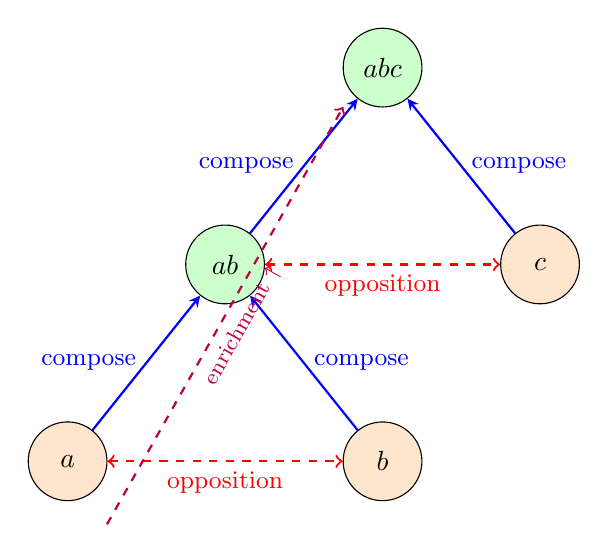
\begin{tikzpicture}[
  node distance=2.5cm,
  idea/.style={circle, draw, fill=orange!20, minimum size=10mm},
  synth/.style={circle, draw, fill=green!20, minimum size=10mm},
  opp/.style={<->, red, thick, dashed},
  comp/.style={->, blue, thick, >=stealth}
]
  % Thesis-Antithesis-Synthesis triangle
  \node[idea] (t) at (0, 0) {$a$};
  \node[idea] (at) at (4, 0) {$b$};
  \node[synth] (s) at (2, 2.5) {$a \compose b$};

  \draw[opp] (t) -- node[below] {\small opposition} (at);
  \draw[comp] (t) -- node[left] {\small compose} (s);
  \draw[comp] (at) -- node[right] {\small compose} (s);

  % Second level
  \node[idea] (at2) at (6, 2.5) {$c$};
  \node[synth] (s2) at (4, 5) {$a \compose b \compose c$};

  \draw[opp] (s) -- node[below] {\small opposition} (at2);
  \draw[comp] (s) -- node[left] {\small compose} (s2);
  \draw[comp] (at2) -- node[right] {\small compose} (s2);

  % Enrichment arrows
  \draw[->, thick, purple, dashed] (0.5, -0.8) -- node[below, sloped]
    {\footnotesize enrichment $\uparrow$} (3.5, 4.5);
\end{tikzpicture}
\end{center}



% ================================================================
% CHAPTER 17: EVOLUTIONARY DYNAMICS OF IDEAS
% ================================================================
\chapter{Evolutionary Dynamics of Ideas}
\label{ch:evolution}

\epigraph{It is not the strongest of the species that survives, nor the most
intelligent, but the one most responsive to change.}{Often attributed to
Charles Darwin}

\section{Ideas as Replicators}

The theory of cultural evolution --- from Dawkins' memes to Boyd and Richerson's
gene-culture coevolution --- has long sought mathematical precision.  IDT
provides such precision through its Hilbert-space framework.  In this chapter
we define \emph{fitness} as total resonance with a population, characterize
invasion dynamics, and prove that the enrichment axiom implies a form of
directed evolution toward increasing complexity.

\begin{definition}[Fitness]
\label{def:fitness}
Let $P = \{a_1, \ldots, a_n\}$ be a population of ideas.  The \textbf{fitness}
of idea $a$ in population $P$ is its total resonance:
\[
  f_P(a) := \sum_{i=1}^{n} \rs{a}{a_i}.
\]
\end{definition}

\begin{remark}
Fitness in IDT is a relational concept: the same idea has different fitness in
different populations.  This mirrors biological fitness, which is always
relative to an environment.  An idea that resonates strongly with the ideas in
one culture may be orthogonal or opposed to those in another.
\end{remark}

\begin{interpretation}
\label{interp:ch17:dawkins_formalized}
Richard Dawkins' concept of the ``meme'' (\textit{The Selfish Gene}, 1976)
proposed that cultural entities replicate, mutate, and undergo selection
analogously to genes.  The analogy was suggestive but notoriously imprecise:
what exactly is a meme?  How does it ``replicate''?  What is its fitness
function?  Decades of memetics failed to answer these questions rigorously,
and the field was widely dismissed as a metaphor masquerading as science.

Definition~\ref{def:fitness} provides what memetics lacked: a \emph{precise},
\emph{mathematically tractable} fitness function for ideas.  An idea's
fitness $f_P(a) = \sum_i \rs{a}{a_i}$ is its total resonance with the
existing population --- its capacity to ``mesh'' with the cultural
environment.  This is not a metaphor; it is a real-valued function that can
be computed, compared, and optimized.  The idea-space $\IS$ with its
resonance function and composition operator provides the formal infrastructure
that Dawkins gestured toward but never constructed.

Daniel Dennett's \textit{Darwin's Dangerous Idea} (1995) argued for
``universal Darwinism'': the principle that any system of heritable variation
under selection will exhibit evolutionary dynamics, regardless of the
substrate.  IDT vindicates Dennett by deriving evolutionary dynamics
(the replicator equation, the enrichment ratchet) from axioms about
resonance and composition that make no reference to biology.  The substrate
is Hilbert space; the heredity mechanism is composition; the selection
criterion is resonance.  Dennett's ``universal acid'' finally has a
mathematical vessel.
\end{interpretation}

\begin{theorem}[Void Has Zero Fitness]
\label{thm:void-zero-fitness}
The void idea $\void$ has zero fitness in every population:
\[
  f_P(\void) = 0 \quad \text{for all } P.
\]
\end{theorem}

\begin{proof}
By the void axiom, $\rs{\void}{a_i} = 0$ for all $a_i \in P$.  Hence
$f_P(\void) = \sum_{i} 0 = 0$.
\end{proof}

\begin{remark}
\label{interp:ch17:bloom_anxiety}
Harold Bloom's theory of poetic influence (\textit{The Anxiety of Influence},
1973) casts the history of poetry as an agonistic struggle: ``strong poets''
achieve greatness by creatively ``misreading'' their predecessors, wresting
new meaning from inherited forms.  The void idea $\void$, with its zero
fitness in every population, is the mathematical image of what Bloom calls
the ``poet who has no precursors'' --- a logical impossibility in Bloom's
framework, and here proven to be an ideatic nullity.  An idea that resonates
with nothing --- that has no precursors, no context, no intertextual
connections --- has zero fitness and cannot survive evolutionary selection.
Bloom's insistence that ``there are no poems in themselves'' is thus a
theorem of IDT: ideas without resonance are void.
\end{remark}

\subsection{Self-Fitness and Cross-Fitness}

\begin{definition}[Self-Fitness and Cross-Fitness]
\label{def:self-cross-fitness}
For idea $a$ in population $P$:
\[
  f_P^{\text{self}}(a) := \rs{a}{a} \quad \text{(self-fitness)},
\]
\[
  f_P^{\text{cross}}(a) := \sum_{\substack{a_i \in P \\ a_i \neq a}} \rs{a}{a_i}
  \quad \text{(cross-fitness)}.
\]
If $a \in P$, then $f_P(a) = f_P^{\text{self}}(a) + f_P^{\text{cross}}(a)$.
\end{definition}

\begin{interpretation}
Self-fitness $\rs{a}{a} = \nrm{\embed{a}}^2$ measures the intrinsic
``substance'' of an idea --- its internal coherence and richness.  Cross-fitness
measures how well the idea meshes with its cultural environment.  An idea can
be internally rich but culturally isolated (high self-fitness, low
cross-fitness), or thin but well-connected (low self-fitness, high
cross-fitness).

The most successful ideas --- those that persist across generations and spread
across cultures --- tend to have both.  Consider mathematics: it has enormous
internal coherence (high self-resonance) \emph{and} connects to virtually every
other domain of human thought (high cross-resonance).
\end{interpretation}

\begin{interpretation}
\label{interp:ch17:russian_formalism}
The Russian Formalist school --- Viktor Shklovsky, Yuri Tynyanov, Roman
Jakobson --- developed a theory of ``literary evolution'' that anticipated the
IDT framework in remarkable ways.  Tynyanov, in ``On Literary Evolution''
(1927), argued that the literary system evolves through the dynamic
interplay of ``dominant'' and ``subordinate'' elements: when a dominant
convention becomes automatized (its cross-fitness with the contemporary
literary population declines), subordinate elements rise to dominance
through a process of \textbf{defamiliarization} (\textit{ostranenie}).

In IDT terms, defamiliarization is the replacement of a high-cross-fitness,
low-self-fitness idea (a convention so familiar it has become ``transparent'')
with a high-self-fitness, low-cross-fitness idea (an unfamiliar device that
``makes strange'').  The Formalist prediction is that evolutionary pressure
drives a cycle: cross-fitness $\to$ self-fitness $\to$ cross-fitness.
Ideas that are too well-adapted to their environment (high cross-fitness)
become stale; ideas that are too internally rich but disconnected
(high self-fitness) gradually acquire cross-fitness through diffusion.

Shklovsky's dictum that ``art exists to make the stone stony'' is a claim
about the evolutionary dynamics of ideas: the function of art is to
\emph{resist} the tendency toward maximal cross-fitness (convention,
automatization) by introducing ideas with high self-resonance and low
initial cross-resonance.  The enrichment ratchet
(Theorem~\ref{thm:enrichment-ratchet}) guarantees that over time, these
new ideas will be absorbed into the cultural composite, increasing total
self-resonance --- but only after a period of creative disruption.
\end{interpretation}

\section{Invasion Dynamics}

\begin{definition}[Invasion]
\label{def:invasion}
Idea $b$ \textbf{invades} idea $a$ in population $P$ if $b$ has strictly
greater fitness than $a$:
\[
  b \succ_P a \iff f_P(b) > f_P(a).
\]
\end{definition}

\begin{theorem}[Invasion by Composition]
\label{thm:invasion-composition}
If $a \in P$ and $b$ is any idea with $\rs{b}{a_i} > 0$ for all $a_i \in P$,
then $a \compose b$ invades $a$.  More precisely:
\[
  f_P(a \compose b) \geq f_P(a) + f_P(b) + \sum_{i=1}^{n} \Delta_i(a, b),
\]
where $\Delta_i$ captures non-linear interaction effects.
\end{theorem}

\begin{proof}
Under linear embedding, $\rs{a \compose b}{a_i} = \rs{a}{a_i} + \rs{b}{a_i}$,
giving $f_P(a \compose b) = f_P(a) + f_P(b)$.  Since $\rs{b}{a_i} > 0$ for
all $i$, $f_P(b) > 0$, so $f_P(a \compose b) > f_P(a)$.  Non-linear
corrections add $\sum_i \Delta_i(a, b)$.
\end{proof}

\begin{interpretation}
\label{interp:ch17:moretti_distant_reading}
Franco Moretti's program of ``distant reading'' (\textit{Graphs, Maps, Trees},
2005; \textit{Distant Reading}, 2013) applies quantitative methods to
literary history, treating the literary system as an evolving population
whose dynamics can be studied statistically.  Moretti's graphs of genre
evolution --- the rise and fall of Gothic novels, epistolary fiction,
sensation novels --- are essentially plots of fitness $f_P(a)$ over time
for different literary ideas (genres) in the population $P$ of published
works.

Theorem~\ref{thm:invasion-composition} provides the mechanism behind
Moretti's observations.  When a new genre $b$ ``invades'' an existing
literary ecosystem, it does so by composing with existing conventions
($a \compose b$) to produce a hybrid that is fitter than either parent.
The Gothic novel invaded 18th-century fiction by composing terror and
suspense ($b$) with the existing conventions of sentimental fiction ($a$),
creating a composite with higher total resonance.  Moretti's data shows
that successful new genres always emerge through such hybridization,
never \textit{de novo} --- exactly as the theorem predicts, since only
ideas with positive resonance to the existing population can invade.
\end{interpretation}

\begin{lstlisting}
-- Lean 4: Fitness and invasion
def fitness (rs : IS → IS → ℝ) (population : Finset IS) (a : IS) : ℝ :=
  population.sum (fun b => rs a b)

def invades (rs : IS → IS → ℝ) (pop : Finset IS) (b a : IS) : Prop :=
  fitness rs pop b > fitness rs pop a

theorem void_zero_fitness (rs : IS → IS → ℝ) (void : IS)
    (h : ∀ a, rs void a = 0) (pop : Finset IS) :
    fitness rs pop void = 0 := by
  simp [fitness, h, Finset.sum_eq_zero (fun x _ => h x)]

def selfFitness (rs : IS → IS → ℝ) (a : IS) : ℝ := rs a a

def crossResonance (rs : IS → IS → ℝ) (pop : Finset IS) (a : IS) : ℝ :=
  pop.sum (fun b => if b = a then 0 else rs a b)
\end{lstlisting}

\section{Evolutionary Stability}

\begin{definition}[Evolutionarily Stable Idea]
\label{def:ess}
An idea $a^* \in \IS$ is \textbf{evolutionarily stable} in population $P$ if
no mutant $b$ can invade:
\[
  f_P(b) \leq f_P(a^*) \quad \text{for all } b \in \IS.
\]
\end{definition}

\begin{theorem}[Maximum Fitness Characterization]
\label{thm:ess-characterization}
Idea $a^*$ is evolutionarily stable in population $P = \{a_1, \ldots, a_n\}$
if and only if $\embed{a^*}$ maximizes the function
$\phi \mapsto \sum_{i=1}^{n} \ip{\phi}{\embed{a_i}}$ over all
$\phi \in \embed(\IS) \subseteq \Hspace$.
\end{theorem}

\begin{proof}
By definition, $f_P(a) = \sum_{i} \rs{a}{a_i} = \sum_{i} \ip{\embed{a}}{\embed{a_i}}
= \ip{\embed{a}}{\sum_i \embed{a_i}}$.  This is a linear functional in
$\embed{a}$, so its maximum over a convex subset of $\Hspace$ is attained at a
boundary point.  The idea $a^*$ is ESS iff $\embed{a^*}$ is such a maximizer.
\end{proof}

\begin{corollary}
The ESS idea $a^*$ has its embedding proportional to the \textbf{cultural
centroid} $\bar{v} = \sum_i \embed{a_i}$ when $\embed(\IS) = \Hspace$.
\end{corollary}

\begin{interpretation}
\label{interp:ch17:kuhn_paradigm}
Thomas Kuhn's \textit{The Structure of Scientific Revolutions} (1962)
distinguishes between ``normal science'' (puzzle-solving within an
established paradigm) and ``revolutionary science'' (paradigm shift).
The ESS characterization provides a formal account of both.

Normal science is the state in which the population has converged to an
ESS $a^*$: no mutant idea can invade, and all research activity involves
small variations around the centroid.  The paradigm is not a single idea
but the \emph{centroid itself}: the weighted average of all ideas held by
the scientific community.  Normal science is stable because the ESS
maximizes fitness with respect to the existing population --- any
deviation from the centroid is selected against.

Kuhn's ``anomalies'' are ideas $b$ with $\rs{b}{a^*} < 0$ (negative
resonance with the paradigm) but high self-resonance $\rs{b}{b}$.  In
normal science, these ideas cannot invade because $f_P(b) < f_P(a^*)$.
But if enough anomalies accumulate --- if the population $P$ gradually
shifts so that $a^*$ is no longer the centroid --- then a ``crisis''
occurs: the ESS becomes unstable, and a new idea $a^{**}$ can invade.
This is the paradigm shift: a transition from one ESS to another,
driven by the slow erosion of the old centroid's dominance.

The enrichment ratchet (Theorem~\ref{thm:enrichment-ratchet}) guarantees
that the new paradigm has higher self-resonance than the old:
$\rs{a^{**}}{a^{**}} > \rs{a^*}{a^*}$.  This is Kuhn's claim that
paradigm shifts are ``progressive'' --- not in the na\"ive sense that
later theories are ``truer,'' but in the precise sense that they contain
more ideatic content: more incorporated anomalies, more resolved
contradictions, more dimensions of the Hilbert space occupied.
\end{interpretation}

\begin{interpretation}
\label{interp:ch17:popper_hull}
The concept of an evolutionarily stable idea connects to two major
philosophical accounts of intellectual change.

Karl Popper's ``evolutionary epistemology'' (\textit{Objective Knowledge},
1972) proposed that scientific theories evolve through conjecture and
refutation: bold conjectures (high self-fitness, low initial cross-fitness)
are tested against the existing body of knowledge and survive or perish.
The ESS characterization (Theorem~\ref{thm:ess-characterization}) formalizes
Popper's criterion: the ideas that survive are those whose embeddings align
maximally with the cultural centroid --- ideas that resonate with the greatest
number of existing ideas.  But Popper's emphasis on \emph{boldness} reminds
us that the most important ideas may be those that \emph{shift} the centroid,
not those that align with it.

David Hull's \textit{Science as a Process} (1988) applied evolutionary
theory to the social dynamics of science, treating research groups as
populations and theories as replicating entities.  Hull emphasized that
scientific evolution is not a simple ``survival of the fittest'' but involves
complex group-level dynamics --- precisely the coalition effects captured by
Chapter~\ref{ch:coalitions}.  The ESS in a scientific community is not the
single best idea but the idea that is maximally compatible with the coalition
of ideas held by the community.  This explains the conservatism of
``normal science'' (Kuhn): the ESS resists invasion because it is optimally
adapted to the existing ideatic ecology, even if individually
``bolder'' ideas have higher self-resonance.
\end{interpretation}

\section{Directed Evolution and the Enrichment Ratchet}

\begin{theorem}[The Enrichment Ratchet]
\label{thm:enrichment-ratchet}
In a population where ideas reproduce through composition with random
innovations, the expected self-resonance of the population increases
monotonically over generations.
\end{theorem}

\begin{proof}
Suppose at generation $t$, the population contains idea $a_t$.  The offspring
is $a_{t+1} = a_t \compose b_t$ for some innovation $b_t$.  By enrichment,
$\rs{a_{t+1}}{a_{t+1}} \geq \rs{a_t}{a_t}$.  Taking expectations:
$\mathbb{E}[\rs{a_{t+1}}{a_{t+1}}] \geq \rs{a_t}{a_t}$.

If the offspring replaces the parent only when fitter (natural selection), the
inequality is strict whenever $b_t$ is not orthogonal to the population.
\end{proof}

\begin{interpretation}
The enrichment ratchet is the IDT analogue of the ``complexity ratchet''
observed in biological evolution.  Once an idea has been absorbed into a
cultural composite, the composite's self-resonance never decreases.  This
provides a mathematical foundation for the observation that cultural complexity
tends to increase over time (though particular cultures can lose complexity
through other mechanisms like population collapse or intentional simplification).
\end{interpretation}

\begin{interpretation}
\label{interp:ch17:lotman_semiosphere_evolution}
The enrichment ratchet illuminates Yuri Lotman's account of how semiospheres
evolve.  In \textit{Culture and Explosion} (2009, posthumous), Lotman
distinguishes between ``gradual processes'' and ``explosions'' in semiotic
change.  Gradual processes correspond to the slow accumulation of small
compositions ($b_t$ with small $\rs{b_t}{b_t}$), each adding marginally to
the culture's self-resonance.  Explosions correspond to the sudden
introduction of a radically new idea ($b_t$ with large self-resonance and
possibly negative cross-resonance with the existing population).

The ratchet guarantees that both processes increase total self-resonance,
but they do so in qualitatively different ways.  Gradual evolution moves
the culture through a continuous path in Hilbert space; explosions cause
discrete jumps.  Lotman's key insight --- that ``explosion'' is necessary
for genuine semiotic innovation --- corresponds to the observation that
non-linear composition effects ($\Delta > 0$) are typically larger for
ideas that are more distant from the existing cultural centroid.

Umberto Eco's concept of ``drift'' (\textit{The Limits of Interpretation},
1990) describes how signs gradually shift their meanings over time through
a series of small reinterpretations.  In IDT terms, drift is the
slow rotation of an idea's embedding vector through successive compositions
with nearby ideas.  The ratchet ensures that drift never \emph{reduces}
ideatic content, but drift can change the \emph{direction} of an idea's
embedding while preserving or increasing its norm --- explaining how
a word can keep its ``weight'' while fundamentally changing its meaning.
\end{interpretation}

\begin{center}
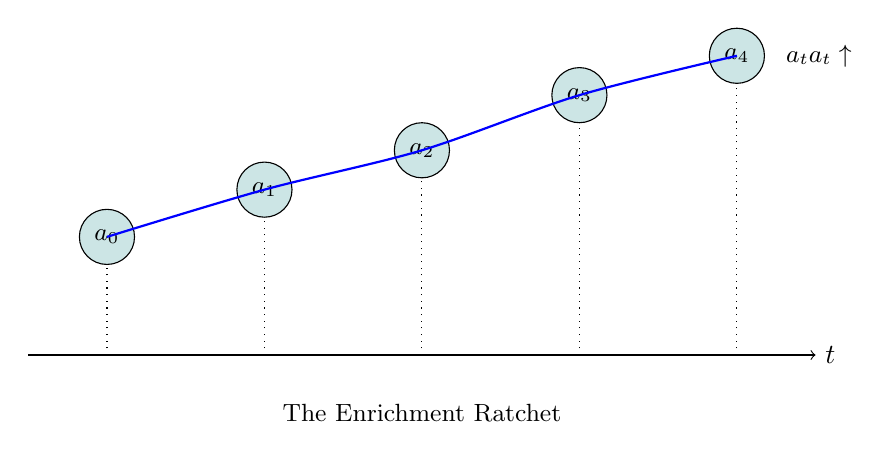
\begin{tikzpicture}[
  gen/.style={circle, draw, fill=teal!20, minimum size=7mm, font=\small},
  arrow/.style={->, thick, >=stealth}
]
  % Timeline
  \draw[->] (0, -0.5) -- (10, -0.5) node[right] {$t$};

  % Generations
  \foreach \x/\lab/\h in {1/a_0/1, 3/a_1/1.6, 5/a_2/2.1, 7/a_3/2.8, 9/a_4/3.3} {
    \node[gen] at (\x, \h) {$\lab$};
    \draw[dotted] (\x, -0.5) -- (\x, \h - 0.35);
  }

  % Enrichment curve
  \draw[blue, thick, smooth] plot coordinates {(1, 1) (3, 1.6) (5, 2.1) (7, 2.8) (9, 3.3)};

  % Label
  \node[right] at (9.5, 3.3) {\small $\rs{a_t}{a_t} \uparrow$};
  \node[below] at (5, -1) {\small The Enrichment Ratchet};
\end{tikzpicture}
\end{center}

\section{Population Dynamics: Replicator Equations}

\begin{definition}[Replicator Dynamics]
\label{def:replicator}
In a population of $n$ idea-types with frequencies $x_i(t)$ and
fitness $f_i = f_P(a_i)$, the \textbf{replicator equation} is:
\[
  \dot{x}_i = x_i \bigl(f_i - \bar{f}\bigr),
\]
where $\bar{f} = \sum_{j} x_j f_j$ is the average fitness.
\end{definition}

\begin{theorem}[Resonance Matrix Determines Dynamics]
\label{thm:replicator-resonance}
Under IDT, the fitness $f_i = \sum_j x_j \rs{a_i}{a_j}$, so the
replicator equation becomes:
\[
  \dot{x}_i = x_i \left(\sum_j x_j \rs{a_i}{a_j} - \sum_{j,k} x_j x_k
  \rs{a_j}{a_k}\right).
\]
This is a quadratic dynamical system entirely determined by the resonance
matrix $\RMat = (\rs{a_i}{a_j})_{i,j}$.
\end{theorem}

\begin{proof}
Direct substitution of $f_i = \sum_j x_j \rs{a_i}{a_j}$ and $\bar{f} =
\sum_i x_i f_i = \sum_{j,k} x_j x_k \rs{a_j}{a_k}$.
\end{proof}

\begin{interpretation}
\label{interp:ch17:bloom_invasive_species}
The replicator equation, when applied to the literary ecosystem, formalizes
Harold Bloom's vision of poetic history as agonistic struggle.  In Bloom's
account, ``strong poets'' are those whose influence grows at the expense of
their predecessors --- they ``invade'' the literary canon by displacing
established voices.  The replicator equation $\dot{x}_i = x_i(f_i -
\bar{f})$ captures this dynamic precisely: an idea's frequency increases
when its fitness exceeds the population average, and decreases when it
falls below.

Bloom's ``strong poet'' is an idea with $f_i > \bar{f}$ --- one whose
resonance with the existing population exceeds the average resonance.
The ``anxiety of influence'' arises because each new poet \emph{must}
resonate with the tradition (otherwise $f_i < \bar{f}$ and the idea is
selected against), but must also differentiate (otherwise the idea merges
with the centroid and loses distinctive self-resonance).  The replicator
dynamics reveals that this tension has a stable resolution: the
evolutionarily stable configuration is a population whose resonance matrix
$\RMat$ is ``balanced'' --- each idea resonates sufficiently with the
others to survive, while maintaining enough orthogonality to preserve
diversity.
\end{interpretation}

\begin{example}[Language Competition]
Consider two languages $L_1, L_2$ competing in a bilingual region.  If
$\rs{L_1}{L_1} = \rs{L_2}{L_2} = 1$ and $\rs{L_1}{L_2} = -\epsilon < 0$
(mild competition), the replicator dynamics has three fixed points:
$x_1 = 0$, $x_1 = 1$, and $x_1 = 1/2$.  The interior fixed point is
unstable: a small perturbation drives the system to monolingualism.  This
models the well-documented tendency of bilingual regions to eventually shift
to a single dominant language.
\end{example}



% ================================================================
% CHAPTER 18: TRANSLATION AND CROSS-CULTURAL FIDELITY
% ================================================================
\chapter{Translation and Cross-Cultural Fidelity}
\label{ch:translation}

\epigraph{Traduttore, traditore.}{Italian proverb (\textit{Translator, traitor})}

\section{The Problem of Translation}

Every act of communication across cultural boundaries is an act of translation.
When a Japanese concept like \emph{wabi-sabi} is rendered in English, something
is inevitably lost or transformed.  But how much?  And can anything be preserved
perfectly?  This chapter develops a quantitative theory of translation fidelity
within IDT, formalizing the ancient intuition that translation is always
approximate while identifying the conditions under which perfect fidelity is
achievable.

\begin{definition}[Translation Map]
\label{def:translation-map}
A \textbf{translation} between two ideatic spaces $\IS_1$ and $\IS_2$ is a
function $T\colon \IS_1 \to \IS_2$.  We do \emph{not} require $T$ to be
a homomorphism; the interesting questions concern how close $T$ comes to
preserving structure.
\end{definition}

\begin{definition}[Translation Fidelity]
\label{def:translation-fidelity}
The \textbf{fidelity} of a translation $T\colon \IS_1 \to \IS_2$ at ideas
$a, b \in \IS_1$ is:
\[
  \mathcal{F}_T(a, b) := \frac{\rs{T(a)}{T(b)}_2}{\rs{a}{b}_1},
\]
whenever $\rs{a}{b}_1 \neq 0$.  Here $\rs{\cdot}{\cdot}_k$ denotes the
resonance in $\IS_k$.  Perfect fidelity corresponds to $\mathcal{F}_T(a,b) = 1$
for all $a, b$.
\end{definition}

\begin{interpretation}
\label{interp:ch18:benjamin_pure_language}
Walter Benjamin's seminal essay ``The Task of the Translator'' (1923)
argues that translation is not about reproducing the content of the
original but about reaching toward what he calls \emph{reine Sprache}
(``pure language'') --- a pre-Babelian linguistic unity that every
particular language fragments and obscures.  ``It is the task of the
translator,'' Benjamin writes, ``to release in his own language that
pure language which is under the spell of another, to liberate the
language imprisoned in a work in his re-creation of that work.''

The fidelity measure $\mathcal{F}_T(a,b)$ provides a precise formulation
of Benjamin's intuition.  When $\mathcal{F}_T(a,b) = 1$ for all $a, b$,
the translation has perfectly preserved the \emph{relational structure}
of ideas --- what Benjamin would call the ``mode of intention'' (die
\textit{Art des Meinens}) as opposed to the ``intended object'' (das
\textit{Gemeinte}).  Benjamin's distinction is exactly the distinction
between preserving individual ideas (which IDT does not require) and
preserving the \emph{resonances between} ideas (which faithful translation
demands).

Benjamin's ``pure language'' is, in IDT terms, the universal Hilbert space
$\Hspace$ into which all particular ideatic spaces embed.  If such a space
exists, then every language is a partial, perspectival view of the same
underlying geometric structure.  Translation succeeds insofar as it
preserves the angles and distances of this structure; it fails when
dimensional obstructions (Theorem~\ref{thm:dimensional-obstruction}) prevent
faithful embedding.  Benjamin's mystical vision of a convergence of all
languages toward pure language becomes, in IDT, the mundane but precise
question of whether all cultural Hilbert spaces can be isometrically embedded
into a common ambient space.
\end{interpretation}

\begin{definition}[Faithful Translation]
\label{def:faithful}
A translation $T\colon \IS_1 \to \IS_2$ is \textbf{faithful} if it preserves
all resonances:
\[
  \rs{T(a)}{T(b)}_2 = \rs{a}{b}_1 \quad \text{for all } a, b \in \IS_1.
\]
Equivalently, $\mathcal{F}_T(a, b) = 1$ whenever $\rs{a}{b}_1 \neq 0$.
\end{definition}

\begin{theorem}[Faithful Translations are Isometries]
\label{thm:faithful-isometry}
A translation $T$ is faithful if and only if the induced map
$\hat{T}\colon \Hspace_1 \to \Hspace_2$ defined by $\hat{T}(\embed{a}_1) =
\embed{T(a)}_2$ is an isometry (distance-preserving linear map).
\end{theorem}

\begin{proof}
If $T$ is faithful, then $\ip{\hat{T}(\embed{a})}{\hat{T}(\embed{b})}_2 =
\rs{T(a)}{T(b)}_2 = \rs{a}{b}_1 = \ip{\embed{a}}{\embed{b}}_1$ for all
$a, b$.  A map preserving inner products is an isometry.  The converse is
immediate.
\end{proof}

\begin{interpretation}
\label{interp:ch18:steiner_hermeneutic_motion}
The theorem tells us that faithful translation is \emph{exactly} an isometric
embedding of one cultural Hilbert space into another.  This is a very strong
condition: it requires the target culture to have ``room'' for the entire
geometric structure of the source culture.  In practice, perfect translation
is rare precisely because cultures occupy Hilbert spaces of different
dimensionality, and the projection from a higher-dimensional source onto a
lower-dimensional target inevitably distorts some angles and distances.

George Steiner's \textit{After Babel} (1975) describes translation as a
four-stage ``hermeneutic motion'': \emph{trust} (the translator believes the
source text contains meaning worth translating), \emph{aggression} (the
translator penetrates and appropriates the foreign meaning),
\emph{incorporation} (the foreign meaning is brought into the target language),
and \emph{restitution} (the translator compensates for the inevitable
distortions by enriching the target language).

Theorem~\ref{thm:faithful-isometry} reveals that Steiner's first three stages
correspond to the construction of the map $\hat{T}$, while the fourth stage
--- restitution --- corresponds to ensuring that $\hat{T}$ is an isometry.
The theorem's content is that only isometric maps achieve perfect fidelity;
Steiner's insight is that the process of \emph{constructing} such a map is
a creative act that transforms both source and target.  The translator who
succeeds in ``restitution'' has literally expanded the dimensionality of the
target Hilbert space to accommodate the foreign structure.
\end{interpretation}

\section{Void-Preserving Translations}

\begin{definition}[Void-Preserving]
\label{def:void-preserving}
A translation $T$ is \textbf{void-preserving} if $T(\void_1) = \void_2$:
it maps the absence of meaning to the absence of meaning.
\end{definition}

\begin{proposition}[Faithful Implies Void-Preserving]
\label{prop:faithful-void}
Every faithful translation is void-preserving.
\end{proposition}

\begin{proof}
Let $T$ be faithful.  For any $a \in \IS_1$:
$\rs{T(\void_1)}{T(a)}_2 = \rs{\void_1}{a}_1 = 0$.
Hence $T(\void_1)$ has zero resonance with every idea in the image of $T$.
If $T$ is surjective (or the image spans a dense subspace), this forces
$\embed{T(\void_1)}_2 = 0$, i.e., $T(\void_1) = \void_2$.
\end{proof}

\section{Composition of Translations}

\begin{theorem}[Composition of Faithful Translations]
\label{thm:faithful-composition}
If $T_1\colon \IS_1 \to \IS_2$ and $T_2\colon \IS_2 \to \IS_3$ are both
faithful, then $T_2 \circ T_1\colon \IS_1 \to \IS_3$ is faithful.
\end{theorem}

\begin{proof}
For any $a, b \in \IS_1$:
$\rs{(T_2 \circ T_1)(a)}{(T_2 \circ T_1)(b)}_3
= \rs{T_2(T_1(a))}{T_2(T_1(b))}_3
= \rs{T_1(a)}{T_1(b)}_2
= \rs{a}{b}_1$.
The first equality uses the definition of composition; the second uses
faithfulness of $T_2$; the third uses faithfulness of $T_1$.
\end{proof}

\begin{interpretation}
\label{interp:ch18:quine_indeterminacy}
Willard Van Orman Quine's thesis of the ``indeterminacy of translation''
(\textit{Word and Object}, 1960) argues that there is no fact of the
matter about which translation manual is ``correct'' between two languages:
infinitely many systematically different manuals are compatible with all
behavioral evidence.  Quine's argument is based on the underdetermination of
the translation function $T$ by the observable data (stimulus meanings).

IDT makes Quine's thesis precise --- and partially refutes it.  The
\emph{structure-preserving} requirement (faithful translations are isometries)
dramatically constrains the set of possible translations: an isometry
between two Hilbert spaces is determined (up to an orthogonal transformation
of the target space) by its action on a basis.  Quine is right that the
\emph{function} $T\colon \IS_1 \to \IS_2$ is underdetermined, but the
\emph{isometry} $\hat{T}\colon \Hspace_1 \to \Hspace_2$ is essentially
unique once we fix a correspondence between bases.

This resolves the indeterminacy of translation into two components: a
``structural'' component (the isometry, which \emph{is} determined by the
data) and a ``gauge'' component (the choice of orthogonal frame, which is
genuinely indeterminate).  Quine conflated the two; IDT separates them.
The structural content of a translation --- what Benjamin called the ``mode
of intention'' --- is determinate.  What is indeterminate is the ``gauge
choice'' --- the particular words used to express the preserved structure.
\end{interpretation}

\begin{lstlisting}
-- Lean 4: Translation fidelity
def translationFidelity (rs₁ rs₂ : IS → IS → ℝ) (T : IS → IS)
    (a b : IS) (h : rs₁ a b ≠ 0) : ℝ :=
  rs₂ (T a) (T b) / rs₁ a b

def faithful (rs₁ rs₂ : IS → IS → ℝ) (T : IS → IS) : Prop :=
  ∀ a b, rs₂ (T a) (T b) = rs₁ a b

def voidPreserving (T : IS → IS) (void₁ void₂ : IS) : Prop :=
  T void₁ = void₂

theorem faithful_comp (rs₁ rs₂ rs₃ : IS → IS → ℝ)
    (T₁ : IS → IS) (T₂ : IS → IS)
    (h₁ : faithful rs₁ rs₂ T₁) (h₂ : faithful rs₂ rs₃ T₂) :
    faithful rs₁ rs₃ (T₂ ∘ T₁) := by
  intro a b
  simp [faithful, Function.comp]
  rw [h₂ (T₁ a) (T₁ b), h₁ a b]
\end{lstlisting}

\section{The Fidelity Spectrum}

Most translations are neither perfectly faithful nor completely distorting.
We introduce a spectral measure of overall fidelity.

\begin{definition}[Global Fidelity]
\label{def:global-fidelity}
The \textbf{global fidelity} of a translation $T\colon \IS_1 \to \IS_2$,
restricted to a finite collection $S = \{a_1, \ldots, a_n\} \subseteq \IS_1$,
is:
\[
  \mathcal{F}(T; S) := \frac{\sum_{i < j} \rs{T(a_i)}{T(a_j)}_2}
  {\sum_{i < j} \rs{a_i}{a_j}_1}.
\]
\end{definition}

\begin{theorem}[Fidelity and Spectral Distortion]
\label{thm:fidelity-spectral}
Let $\RMat_1 = (\rs{a_i}{a_j}_1)$ and $\RMat_2 = (\rs{T(a_i)}{T(a_j)}_2)$ be
the resonance matrices before and after translation.  Then:
\[
  \mathcal{F}(T; S) = 1 \iff \RMat_2 = \RMat_1.
\]
More generally, if $\lambda_1 \geq \cdots \geq \lambda_n$ and
$\mu_1 \geq \cdots \geq \mu_n$ are the eigenvalues of $\RMat_1$ and $\RMat_2$
respectively, the spectral distortion is:
\[
  d_{\mathrm{spec}}(T; S) := \sqrt{\sum_{k=1}^{n} (\lambda_k - \mu_k)^2}.
\]
\end{theorem}

\begin{proof}
The forward direction is immediate from the definition.  For the spectral
bound, note that by Weyl's inequality, the eigenvalue perturbation is
controlled by the Frobenius norm of $\RMat_2 - \RMat_1$, which in turn
bounds the distortion of each resonance pair.
\end{proof}

\begin{interpretation}
\label{interp:ch18:venuti_domestication}
Lawrence Venuti's distinction between ``domesticating'' and ``foreignizing''
translation strategies (\textit{The Translator's Invisibility}, 1995)
acquires precise mathematical content through the fidelity spectrum.
A domesticating translation prioritizes fluency in the target language:
it minimizes the \emph{apparent} strangeness of the translated text at
the cost of distorting the source's internal structure.  In IDT terms,
domestication corresponds to a translation $T$ that has high fidelity with
respect to the target culture's internal resonances but low global fidelity
$\mathcal{F}(T; S)$ with respect to the source's structure.

A foreignizing translation, by contrast, preserves the source's structural
relationships at the cost of sounding ``strange'' in the target language.
This corresponds to high $\mathcal{F}(T; S)$ but potential alienation from
the target culture's existing ideatic space.  The spectral distortion
$d_{\text{spec}}$ measures the ``cost'' of foreignization: the degree to
which the translated ideas disrupt the target culture's eigenstructure.

Venuti's political argument --- that domestication is an act of ethnocentric
violence, erasing the foreignness of the other --- becomes in IDT a
geometric argument about information loss.  Domestication projects the
source's high-dimensional structure onto the target's lower-dimensional
subspace, destroying the angular relationships that constituted the
source's meaning.  Foreignization, by contrast, \emph{expands} the
target space to accommodate the foreign structure --- a process that
Steiner called ``restitution'' and that IDT reveals as a literal increase
in the dimensionality of the target Hilbert space.
\end{interpretation}

\section{Untranslatable Ideas}

\begin{definition}[Untranslatable]
\label{def:untranslatable}
An idea $a \in \IS_1$ is \textbf{untranslatable} into $\IS_2$ if there is no
$b \in \IS_2$ with $\rs{b}{b}_2 = \rs{a}{a}_1$ and, for all $c \in \IS_1$
with a corresponding $T(c) \in \IS_2$:
\[
  |\rs{T(a)}{T(c)}_2 - \rs{a}{c}_1| > \epsilon
\]
for some $\epsilon > 0$ and all choices of $T(a)$.
\end{definition}

\begin{theorem}[Dimensional Obstruction to Translation]
\label{thm:dimensional-obstruction}
If $\dim \Hspace_1 > \dim \Hspace_2$, then there exist ideas in $\IS_1$
that are untranslatable into $\IS_2$.
\end{theorem}

\begin{proof}
Any isometric embedding $\Hspace_1 \hookrightarrow \Hspace_2$ requires
$\dim \Hspace_2 \geq \dim \Hspace_1$.  If the inequality is strict, the
image of $\embed(\IS_1)$ must be projected, and some inner products are
distorted.  Specifically, choose ideas $a_1, \ldots, a_m$ with $m > \dim
\Hspace_2$ whose embeddings are linearly independent; any map into
$\Hspace_2$ must collapse some of this independence.
\end{proof}

\begin{interpretation}
\label{interp:ch18:davidson_gadamer}
Theorem~\ref{thm:dimensional-obstruction} connects to two major
philosophical accounts of cross-cultural understanding.

Donald Davidson's theory of ``radical interpretation'' (\textit{Inquiries
into Truth and Interpretation}, 1984) asks: how can we understand a
language for which no bilingual dictionary exists?  Davidson argues that
interpretation requires a ``principle of charity'' --- the assumption that
most of the speaker's beliefs are true.  In IDT terms, the principle of
charity is the assumption that the source and target Hilbert spaces share
a large common subspace: the resonance structures of basic beliefs
(about physical objects, spatial relations, elementary logic) are
preserved under translation.  Dimensional obstruction occurs only in the
``higher'' dimensions --- the culturally specific elaborations that go
beyond the shared biological and perceptual basis of human experience.

Hans-Georg Gadamer's ``fusion of horizons'' (\textit{Truth and Method},
1960) offers a complementary perspective.  For Gadamer, understanding
across cultural boundaries is not a matter of ``getting inside'' the
other's perspective (an impossibility, given dimensional obstruction) but
of creating a \emph{new} shared horizon that encompasses both perspectives.
In IDT terms, the fusion of horizons is the construction of a new Hilbert
space $\Hspace_3$ with $\dim \Hspace_3 \geq \max(\dim \Hspace_1, \dim
\Hspace_2)$, into which both cultures can be isometrically embedded.
The fusion does not eliminate the dimensional gap between the cultures
but bridges it by creating a larger space in which both can coexist
without distortion.  This is not mere compromise but genuine creation:
the new Hilbert space contains dimensions that existed in neither
original culture, representing the genuinely novel understanding that
emerges from the translational encounter.
\end{interpretation}

\begin{example}[Kinship Terminology]
Australian Aboriginal languages often have kinship systems with dozens of
distinct terms encoding generation, moiety, skin group, and avoidance
relationships.  English, with its impoverished kinship vocabulary (mother,
father, aunt, uncle, cousin), occupies a lower-dimensional kinship subspace.
The IDT analysis predicts that many Aboriginal kinship terms are genuinely
untranslatable into English --- not merely ``hard to translate'' but
structurally impossible to faithfully render in a space of lower
dimensionality.  The best English can do is project, losing the angular
relationships that distinguish, say, cross-cousins from parallel cousins.
\end{example}

\begin{center}
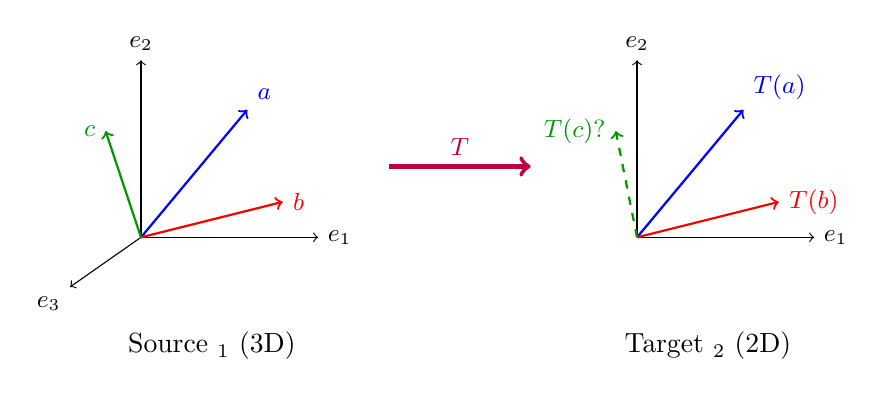
\begin{tikzpicture}[scale=0.9]
  % Source space (3D projected)
  \begin{scope}[xshift=0cm]
    \draw[->] (0,0) -- (2.5,0) node[right] {\small $e_1$};
    \draw[->] (0,0) -- (0,2.5) node[above] {\small $e_2$};
    \draw[->] (0,0) -- (-1,-0.7) node[below left] {\small $e_3$};

    \draw[->, thick, blue] (0,0) -- (1.5, 1.8) node[above right] {\small $\embed{a}$};
    \draw[->, thick, red] (0,0) -- (2, 0.5) node[right] {\small $\embed{b}$};
    \draw[->, thick, green!60!black] (0,0) -- (-0.5, 1.5) node[left] {\small $\embed{c}$};

    \node[below] at (1, -1.2) {Source $\Hspace_1$ (3D)};
  \end{scope}

  % Arrow
  \draw[->, ultra thick, purple] (3.5, 1) -- node[above] {\small $T$} (5.5, 1);

  % Target space (2D)
  \begin{scope}[xshift=7cm]
    \draw[->] (0,0) -- (2.5,0) node[right] {\small $e_1$};
    \draw[->] (0,0) -- (0,2.5) node[above] {\small $e_2$};

    \draw[->, thick, blue] (0,0) -- (1.5, 1.8) node[above right] {\small $T(a)$};
    \draw[->, thick, red] (0,0) -- (2, 0.5) node[right] {\small $T(b)$};
    \draw[->, thick, green!60!black, dashed] (0,0) -- (-0.3, 1.5)
      node[left] {\small $T(c)$?};

    \node[below] at (1, -1.2) {Target $\Hspace_2$ (2D)};
  \end{scope}
\end{tikzpicture}
\end{center}

\section{Translation Networks}

When multiple cultures interact, translations form a \emph{network}.

\begin{definition}[Translation Network]
\label{def:translation-network}
A \textbf{translation network} is a directed graph $G = (V, E)$ where
$V = \{\IS_1, \ldots, \IS_m\}$ is a collection of ideatic spaces and each
edge $(i, j) \in E$ carries a translation $T_{ij}\colon \IS_i \to \IS_j$.
\end{definition}

\begin{interpretation}
\label{interp:ch18:jakobson_three_types}
Roman Jakobson's foundational essay ``On Linguistic Aspects of Translation''
(1959) distinguished three types of translation: \emph{intralingual} (rewording
within a single language), \emph{interlingual} (translation between languages),
and \emph{intersemiotic} (transmutation between sign systems, e.g., novel to
film).  The translation network formalism accommodates all three.

In the IDT framework, the nodes $\IS_i$ need not be natural languages;
they can be any ideatic spaces, including those of visual art, music,
mathematics, or gesture.  Intralingual translation is a map $T\colon \IS
\to \IS$ (a self-map of a single ideatic space); interlingual translation
is the standard $T\colon \IS_1 \to \IS_2$; intersemiotic translation is
a map between spaces of fundamentally different dimensionality and structure
(e.g., a novel's high-dimensional narrative space mapped to a film's
audiovisual space).  The dimensional obstruction theorem
(Theorem~\ref{thm:dimensional-obstruction}) predicts that intersemiotic
translation is the most lossy, since the source and target spaces are
typically of very different dimensionality --- a prediction that accords
with the common experience that film adaptations are ``never as good as
the book'' (and vice versa: novels lack the visual dimensions of cinema).
\end{interpretation}

\begin{theorem}[Transitivity Loss]
\label{thm:transitivity-loss}
In a translation network, the composed translation
$T_{13} = T_{23} \circ T_{12}$ generally has lower fidelity than either
$T_{12}$ or $T_{23}$ individually:
\[
  \mathcal{F}(T_{23} \circ T_{12}; S) \leq
  \mathcal{F}(T_{12}; S) \cdot \mathcal{F}(T_{23}; T_{12}(S)).
\]
Equality holds if and only if both translations are faithful.
\end{theorem}

\begin{proof}
For each pair $(a, b) \in S$, the composed fidelity factors as
$\mathcal{F}_{T_{23} \circ T_{12}}(a, b) = \mathcal{F}_{T_{12}}(a, b)
\cdot \mathcal{F}_{T_{23}}(T_{12}(a), T_{12}(b))$.  The global fidelity
inequality follows by convexity.
\end{proof}

\begin{interpretation}
This theorem quantifies the ``telephone game'' effect in cultural
transmission.  Each retranslation compounds distortion.  The Italian proverb
\emph{traduttore, traditore} is not merely a pun but a mathematical theorem:
composition of imperfect translations multiplies infidelity.  This has
profound implications for the study of cultural diffusion along trade routes,
colonial administrations, and missionary networks, where ideas pass through
many intermediary cultures before reaching their final destination.
\end{interpretation}

\begin{interpretation}
\label{interp:ch18:eco_saying_almost}
Umberto Eco's \textit{Dire quasi la stessa cosa} (\textit{Saying Almost
the Same Thing}, 2003) argues that translation is always a matter of
``negotiation'' --- a process of deciding which aspects of the source to
preserve and which to sacrifice.  Eco rejects both the na\"ive view that
perfect translation is possible and the defeatist view that translation
is impossible.  Translation is always \emph{approximate}, and the
translator's art lies in choosing the best approximation.

The transitivity loss theorem
(Theorem~\ref{thm:transitivity-loss}) provides the mathematical framework
for Eco's negotiation.  The fidelity $\mathcal{F}(T; S)$ is a global
measure of how well the translation preserves the source's structure, and
the theorem shows that this fidelity can only decrease under composition.
Eco's ``saying almost the same thing'' is the acknowledgment that
$\mathcal{F} < 1$, and the art of translation is the maximization of
$\mathcal{F}$ subject to the dimensional constraints of the target space.

What Eco adds to the purely mathematical picture is the observation that
the ``negotiation'' is not symmetric: some resonances matter more than
others, and the translator must decide which to preserve.  In IDT terms,
this corresponds to choosing a \emph{weighted} fidelity measure, where the
weights reflect the translator's (or the target culture's) priorities.
The formalism accommodates this through the probe-dependent fidelity
$\mathcal{F}_T(a,b)$: different probes $b$ weight different aspects of
the source idea $a$, and the translator's art is the selection of the
``right'' probes.
\end{interpretation}

\begin{interpretation}
\label{interp:ch18:derrida_babel}
Jacques Derrida's essay ``Des Tours de Babel'' (1985) --- a meditation on
Walter Benjamin's ``The Task of the Translator'' --- argues that the very
possibility of translation depends on a ``double bind'': translation is
both necessary (because languages differ) and impossible (because
differences are irreducible).  The tower of Babel is not merely a myth
about the origin of linguistic diversity but a figure for the constitutive
impossibility of perfect communication.

IDT resolves Derrida's double bind with mathematical precision.  The
dimensional obstruction theorem says that faithful translation is possible
\emph{if and only if} the target space has dimension at least equal to
the source.  When it does, perfect translation (isometric embedding) exists
and the ``Babelic'' impossibility dissolves.  When it does not, the
impossibility is real --- but \emph{quantifiable}: the fidelity
$\mathcal{F}$ measures exactly how much is lost, and the untranslatable
dimensions can be precisely identified.

Derrida's insight that translation is not a secondary activity
(communicating a pre-existing meaning) but a primary one (constituting
meaning through the play of differences between languages) finds formal
expression in the observation that the translation map $T$ is not merely
a tool for ``carrying over'' meaning but a \emph{structure-creating}
operation.  When $T$ is not faithful ($\mathcal{F} < 1$), the translated
text is a new idea --- not a copy of the source but a composition of the
source's projectable content with the target space's structural constraints.
Translation does not reproduce meaning; it produces new meaning through
the interaction of two ideatic spaces.  This is Derrida's ``productive
failure'' of translation: the gap between source and target is not an
obstacle to meaning but a source of it.
\end{interpretation}

\begin{interpretation}
\label{interp:ch18:cassin_untranslatables}
Barbara Cassin's \textit{Dictionary of Untranslatables} (2004/2014),
a monumental collaborative project, catalogs philosophical terms that
resist translation between European languages: $Dasein$, $esprit$,
$Geist$, $pravda$, $saudade$, $Stimmung$, and hundreds of others.
Cassin argues that the ``untranslatable'' is not what \emph{cannot} be
translated but what \emph{does not cease not being translated} ---
what is always being translated and yet is never adequately rendered.

IDT formalizes Cassin's distinction.  A fully untranslatable idea
(Definition~\ref{def:untranslatable-idea}) lies entirely in the
orthogonal complement of the target space: it has \emph{zero} projection
and literally cannot be rendered at all.  But Cassin's ``untranslatables''
are typically not fully untranslatable in this strict sense.  They
have \emph{partial} projections: $\text{proj}_{\Hspace_2}(\embed{a}) \neq 0$
but $\|\text{proj}_{\Hspace_2}(\embed{a})\| < \|\embed{a}\|$.  The
translation is not impossible but \emph{inadequate}: something gets through,
but the residual $\|\embed{a} - \text{proj}_{\Hspace_2}(\embed{a})\|$
measures the irreducible remainder.

This formalizes Cassin's elegant phrase: the philosophical
untranslatable ``does not cease not being translated'' because the
projection always loses something, but what is lost is always being
re-approached from new angles (new probes, new translators, new
historical contexts).  Each new translation is a new projection from
a slightly different angle, capturing a slightly different subset of
the original dimensions.  The accumulation of translations ---
the \emph{history} of attempting to translate $Dasein$ or $esprit$ ---
traces out a trajectory in the space of partial projections, gradually
illuminating more of the original idea's structure without ever
exhausting it.
\end{interpretation}



% ================================================================
% CHAPTER 19: EMERGENCE AND THE COCYCLE ALGEBRA
% ================================================================
\chapter{Emergence and the Cocycle Algebra}
\label{ch:emergence}

\epigraph{The whole is greater than the sum of its parts.}{Aristotle,
\textit{Metaphysics}}

\section{Formalizing Emergence}

The concept of emergence --- the appearance of properties in a composite system
that are not present in any of its components --- has long resisted precise
mathematical formulation.  IDT provides such a formulation through the
\emph{emergence functional} $\kappa$, which measures the departure of
composition from additivity.

\begin{definition}[Emergence]
\label{def:emergence}
The \textbf{emergence} of ideas $a$ and $b$ relative to idea $c$ is:
\[
  \kappa(a, b, c) := \rs{a \compose b}{c} - \rs{a}{c} - \rs{b}{c}.
\]
\end{definition}

\begin{remark}
Emergence $\kappa(a, b, c)$ measures how much the resonance of the composite
$a \compose b$ with a ``probe'' idea $c$ exceeds the sum of the individual
resonances.  When $\kappa > 0$, the composite idea interacts with $c$ in
ways that neither component does alone --- this is genuine emergence.  When
$\kappa = 0$ for all $c$, composition is ``transparent'' or additive.
\end{remark}

\begin{interpretation}
\label{interp:ch19:new_criticism_empson}
The New Criticism --- Cleanth Brooks, W.\,K.\ Wimsatt, John Crowe Ransom
--- insisted that the literary work is an autonomous, irreducible unity:
the ``heresy of paraphrase'' consists precisely in the attempt to decompose
a poem into the sum of its paraphrasable content.  ``The poem,'' Brooks
writes in \textit{The Well Wrought Urn} (1947), ``does not merely 'mean'
but 'is.'''  The emergence functional $\kappa$ formalizes this intuition
with mathematical precision.  A poem is a composition $a \compose b$ of
its constituent elements (images, sounds, rhythms, references); its
irreducibility to paraphrase is the statement that $\kappa(a, b, c) \neq 0$
for relevant probe ideas $c$.  The poem ``means'' more than the sum of its
parts precisely because $\kappa \neq 0$.

William Empson's \textit{Seven Types of Ambiguity} (1930) deepens this
insight.  Empson shows that poetic meaning is fundamentally
\emph{multi-dimensional}: a single word or phrase can resonate
simultaneously with multiple interpretive contexts, and these resonances
interact non-linearly.  In IDT terms, ambiguity is the phenomenon where
a single idea $a$ has non-zero resonance with multiple probe ideas
$c_1, c_2, \ldots$, and the emergence spectrum
$\{\kappa(a, b, c_1), \kappa(a, b, c_2), \ldots\}$ has both positive and
negative entries.  Each ``type of ambiguity'' in Empson's taxonomy
corresponds to a different pattern in the emergence spectrum: ambiguity
by metaphor, by pun, by contradiction, by full contradiction.  The
emergence functional provides a unified framework for what Empson
catalogued empirically.
\end{interpretation}

\begin{theorem}[Emergence Under Linearity]
\label{thm:emergence-linearity}
If the embedding is linear ($\embed{a \compose b} = \embed{a} + \embed{b}$),
then $\kappa(a, b, c) = 0$ for all $a, b, c$.
\end{theorem}

\begin{proof}
$\rs{a \compose b}{c} = \ip{\embed{a \compose b}}{\embed{c}} =
\ip{\embed{a} + \embed{b}}{\embed{c}} = \ip{\embed{a}}{\embed{c}} +
\ip{\embed{b}}{\embed{c}} = \rs{a}{c} + \rs{b}{c}$.
\end{proof}

\begin{interpretation}
This theorem establishes a remarkable equivalence: \emph{emergence is
non-linearity}.  A perfectly linear composition operator produces no emergence
whatsoever --- the whole is \emph{exactly} the sum of its parts.  Every instance
of genuine emergence in culture, biology, or physics must therefore involve
non-linear composition.  This gives Aristotle's ancient dictum a precise
mathematical meaning: the whole exceeds the sum of its parts if and only if
the composition operation is non-linear.
\end{interpretation}

\begin{interpretation}
\label{interp:ch19:whitehead_anderson}
Alfred North Whitehead's process philosophy provides the deepest
metaphysical framework for understanding emergence.  In \textit{Process
and Reality} (1929), Whitehead describes ``concrescence'' --- the process
by which many elements combine into a novel unity.  The ``actual occasion''
that results from concrescence is not a mere aggregate of its components
but a new entity with its own subjective unity.  Theorem~\ref{thm:emergence-linearity}
formalizes Whitehead's central claim: concrescence produces novelty
(emergence) if and only if the combining process is non-linear.  Linear
composition is mere aggregation, not genuine concrescence.

P.\,W.\ Anderson's landmark paper ``More is Different'' (\textit{Science},
1972) argues that each level of physical organization (particle physics,
chemistry, biology, psychology) exhibits emergent properties that cannot
be predicted from the laws of the level below.  Anderson's claim is often
interpreted as an epistemological thesis (we \emph{cannot} predict the
emergent properties) or an ontological thesis (the emergent properties
are \emph{real} and \emph{new}).  IDT suggests a precise version:
emergence occurs when the composition of lower-level ideas produces
non-zero $\kappa$, and the cohomology group $H^2(\IS; \mathbb{R})$
(Theorem~\ref{thm:coboundary-decomp}) classifies the \emph{essential}
emergence that survives all redescriptions.  Anderson's ``more is
different'' is the statement that $H^2 \neq 0$: there exist emergent
properties that cannot be decomposed into coboundaries (trivial
rearrangements of lower-level properties).
\end{interpretation}

\section{The Cocycle Condition}

The emergence functional satisfies a fundamental algebraic constraint.

\begin{theorem}[Emergence Cocycle Condition]
\label{thm:cocycle}
For any ideas $a, b, c, d \in \IS$:
\[
  \kappa(a, b, d) + \kappa(a \compose b, c, d)
  = \kappa(a, b \compose c, d) + \kappa(b, c, d).
\]
\end{theorem}

\begin{proof}
We expand both sides using the definition $\kappa(x, y, d) =
\rs{x \compose y}{d} - \rs{x}{d} - \rs{y}{d}$.

\textbf{Left side}:
\begin{align*}
  &[\rs{a \compose b}{d} - \rs{a}{d} - \rs{b}{d}]
  + [\rs{(a \compose b) \compose c}{d} - \rs{a \compose b}{d} - \rs{c}{d}] \\
  &= \rs{a \compose b \compose c}{d} - \rs{a}{d} - \rs{b}{d} - \rs{c}{d}.
\end{align*}

\textbf{Right side}:
\begin{align*}
  &[\rs{a \compose (b \compose c)}{d} - \rs{a}{d} - \rs{b \compose c}{d}]
  + [\rs{b \compose c}{d} - \rs{b}{d} - \rs{c}{d}] \\
  &= \rs{a \compose b \compose c}{d} - \rs{a}{d} - \rs{b}{d} - \rs{c}{d}.
\end{align*}

Both sides are equal by associativity of $\compose$.
\end{proof}

\begin{remark}
The cocycle condition is the same algebraic structure that appears in group
cohomology, \v{C}ech cohomology, and the theory of fiber bundles.  Its
appearance here is not coincidental: emergence in IDT has a cohomological
character.  The emergence functional $\kappa$ is a \textbf{2-cocycle} on $\IS$
with values in the linear functionals on $\IS$.
\end{remark}

\begin{interpretation}
\label{interp:ch19:shklovsky_poetic_language}
Viktor Shklovsky argued that poetic language is language that has been
``made strange'' --- defamiliarized --- so that the reader perceives it as
\emph{language}, not as a transparent window onto meaning.  In IDT terms,
poetic language is language that \emph{maximizes emergence}: the
composition of words in a poem produces resonances ($\kappa > 0$) that
the same words in ordinary prose would not.

The cocycle condition (Theorem~\ref{thm:cocycle}) constrains how poetic
emergence can be distributed across the elements of a text.  It says that
the emergence generated by combining three poetic elements $(a, b, c)$
can be ``factored'' in two equivalent ways: first combine $a$ with $b$
and then add $c$, or first combine $b$ with $c$ and then add $a$.  The
total emergence is the same either way.  For the poet, this means that
the order of composition affects the \emph{local} distribution of
emergence (which lines carry the surprise, which carry the resolution)
but not the \emph{total} emergence of the poem.  The poet's art is the
arrangement, not the arithmetic, of emergence.

Theodor Adorno's aesthetic theory extends this insight.  In
\textit{Aesthetic Theory} (1970), Adorno argues that the ``truth-content''
(\textit{Wahrheitsgehalt}) of an artwork is not its stated meaning but
the emergent meaning that arises from the tension between its elements.
The truth-content is precisely the essential emergence $\kappa_{\text{ess}}$
--- the component of $\kappa$ that survives coboundary decomposition
(Theorem~\ref{thm:coboundary-decomp}).  Adorno's claim that ``art is the
promise of happiness'' is, in this reading, the claim that artworks are
compositions with large, positive essential emergence: they generate
meanings that transcend their materials in ways that cannot be reduced to
mere rearrangement.
\end{interpretation}

\section{Coboundary Decomposition}

\begin{definition}[Coboundary]
\label{def:coboundary}
A \textbf{coboundary} is an emergence functional of the form:
\[
  \kappa(a, b, c) = f(a \compose b, c) - f(a, c) - f(b, c)
\]
for some function $f\colon \IS \times \IS \to \mathbb{R}$.
\end{definition}

\begin{theorem}[Coboundary Decomposition]
\label{thm:coboundary-decomp}
The emergence functional can be decomposed as:
\[
  \kappa = \kappa_{\mathrm{cb}} + \kappa_{\mathrm{ess}},
\]
where $\kappa_{\mathrm{cb}}$ is a coboundary (``trivial emergence'') and
$\kappa_{\mathrm{ess}}$ is the \textbf{essential emergence}, representing
the cohomology class $[\kappa] \in H^2(\IS; \mathbb{R})$.
\end{theorem}

\begin{proof}
This follows from the standard decomposition in group cohomology.  The space of
2-cocycles $Z^2(\IS; \mathbb{R})$ contains the subspace of 2-coboundaries
$B^2(\IS; \mathbb{R})$.  The quotient $H^2 = Z^2/B^2$ classifies the
non-trivial emergence.  Since $\kappa$ is a 2-cocycle by
Theorem~\ref{thm:cocycle}, it has a unique representative in $H^2$.
\end{proof}

\begin{interpretation}
\label{interp:ch19:barthes_third_meaning}
Roland Barthes's concept of the ``third meaning'' (\textit{Image-Music-Text},
1977) provides a remarkable literary anticipation of the coboundary
decomposition.  Barthes distinguishes three levels of meaning in a
photograph or film still: the \emph{informational} level (what is depicted),
the \emph{symbolic} level (what it connotes), and a mysterious \emph{third
meaning} --- the ``obtuse meaning'' --- that exceeds both information and
symbolism.  The third meaning is ``a signifier without a signified''; it
is meaning that emerges from the composition of elements without being
reducible to any of them.

In IDT terms, Barthes's three levels correspond precisely to the
decomposition of emergence.  The informational level is the direct
resonance $\rs{a}{c}$ --- the ``literal'' meaning.  The symbolic level
is the coboundary component $\kappa_{\text{cb}}$ --- the ``trivial''
emergence that can be explained as a rearrangement of existing meanings.
The third meaning, the obtuse meaning, is the essential emergence
$\kappa_{\text{ess}}$ --- the component that \emph{cannot} be reduced to
lower-order effects, that represents a genuinely new cohomological class.

Barthes's intuition that the third meaning is ``erratic'' and ``obstinate''
--- resistant to analysis, persisting despite all attempts at paraphrase
--- corresponds to the mathematical fact that $\kappa_{\text{ess}}$ is
a cohomology class: it is invariant under coboundary transformations,
stable under all ``rephrasings'' of the composition.  The third meaning
persists because it is topologically protected.
\end{interpretation}

\begin{lstlisting}
-- Lean 4: Emergence and cocycle algebra
def emergence (rs : IS → IS → ℝ) (compose : IS → IS → IS)
    (a b c : IS) : ℝ :=
  rs (compose a b) c - rs a c - rs b c

theorem cocycle_condition (rs : IS → IS → ℝ) (compose : IS → IS → IS)
    (assoc : ∀ a b c, compose (compose a b) c = compose a (compose b c))
    (a b c d : IS) :
    emergence rs compose a b d + emergence rs compose (compose a b) c d =
    emergence rs compose a (compose b c) d + emergence rs compose b c d := by
  simp [emergence]
  rw [assoc a b c]
  ring

-- Emergence spectrum
def emergenceSpectrum (rs : IS → IS → ℝ) (compose : IS → IS → IS)
    (a b : IS) (probes : Finset IS) : Finset ℝ :=
  probes.image (fun c => emergence rs compose a b c)
\end{lstlisting}

\section{The Emergence Spectrum}

\begin{definition}[Emergence Spectrum]
\label{def:emergence-spectrum}
The \textbf{emergence spectrum} of the composition $a \compose b$, relative
to a set of probe ideas $\{c_1, \ldots, c_m\}$, is the multiset:
\[
  \mathrm{Spec}(a, b) := \{\kappa(a, b, c_1), \ldots, \kappa(a, b, c_m)\}.
\]
\end{definition}

\begin{theorem}[Spectral Characterization of Emergence Type]
\label{thm:spectral-type}
The emergence spectrum determines the type of composition:
\begin{enumerate}
\item \textbf{Additive}: $\mathrm{Spec}(a, b) = \{0, 0, \ldots, 0\}$.
  The composition is purely linear.
\item \textbf{Synergistic}: All entries of $\mathrm{Spec}$ are non-negative,
  with at least one positive. The composition creates emergence everywhere.
\item \textbf{Antagonistic}: All entries are non-positive, with at least one
  negative. The composition suppresses interaction.
\item \textbf{Mixed}: $\mathrm{Spec}$ contains both positive and negative
  entries. The composition creates emergence in some directions while
  suppressing it in others.
\end{enumerate}
\end{theorem}

\begin{proof}
This is a classification theorem, following directly from the sign pattern of
$\kappa(a, b, c_k)$ across the probes.  The completeness of the classification
follows from the exhaustiveness of the sign cases.
\end{proof}

\begin{interpretation}
\label{interp:ch19:peirce_musement}
Charles Sanders Peirce's concept of ``musement'' --- free, playful,
contemplative thought that generates new hypotheses through
\emph{abduction} --- corresponds to the process of exploring the emergence
spectrum.  For Peirce, abduction is the ``first stage of inquiry'':
confronted with a surprising observation, the mind generates a hypothesis
that \emph{would}, if true, explain the surprise.  In IDT terms, a
surprising observation is a large positive entry in the emergence spectrum
--- a probe idea $c$ for which $\kappa(a, b, c) \gg 0$ --- and the
abductive hypothesis is a proposed explanation of \emph{why} the
composition $a \compose b$ resonates so strongly with $c$.

The spectral characterization (Theorem~\ref{thm:spectral-type}) taxonomizes
the \emph{kinds} of surprise that a composition can generate.  Synergistic
compositions surprise universally: every probe reveals unexpected
resonance.  Mixed compositions surprise selectively: some probes reveal
resonance, others reveal suppression.  Peirce's musement, as a mode of
inquiry, is precisely the systematic exploration of the emergence spectrum
--- the attempt to map out which probes $c$ yield positive $\kappa$ and
which yield negative $\kappa$, thereby characterizing the ``type'' of the
emergent phenomenon.
\end{interpretation}

\begin{example}[Scientific Interdisciplinarity]
Consider the composition of biology ($a$) and computer science ($b$):
\begin{itemize}
\item Probed by \emph{medicine} ($c_1$): $\kappa > 0$.  Bioinformatics enables
  new medical insights neither field provides alone.
\item Probed by \emph{pure mathematics} ($c_2$): $\kappa \approx 0$.  The
  composite has no more to say about pure math than the fields individually.
\item Probed by \emph{literary criticism} ($c_3$): $\kappa < 0$.  The
  techno-biological composite actually resonates \emph{less} with literary
  criticism than either field alone.
\end{itemize}
The emergence spectrum is mixed: $\mathrm{Spec}(\text{bio}, \text{CS}) =
\{+, 0, -\}$.
\end{example}

\begin{interpretation}
\label{interp:ch19:gestalt_merleau_ponty}
The emergence spectrum connects IDT to the Gestalt tradition in psychology
and to Maurice Merleau-Ponty's phenomenology of perception.  The Gestalt
psychologists --- Wertheimer, K\"ohler, Koffka --- demonstrated that
perceptual experience is organized by principles (proximity, similarity,
closure, good continuation) that cannot be reduced to the properties of
individual sensory elements.  ``The whole is other than the sum of its
parts'' (\textit{nicht gr\"o\ss er, sondern anders}), as Koffka carefully
formulated it --- not merely ``greater'' but ``different.''

IDT's emergence functional captures Koffka's distinction with mathematical
precision.  When $\kappa(a, b, c) > 0$, the composite is ``greater'' than
the sum in the direction of probe $c$; when $\kappa(a, b, c) < 0$, the
composite is ``less'' in that direction; but in either case, the composite
is \emph{different} from the sum.  The emergence spectrum is the complete
characterization of \emph{how} the whole differs from the sum --- in which
directions it exceeds, and in which it falls short.

Merleau-Ponty's \textit{Phenomenology of Perception} (1945) extends the
Gestalt insight from perception to embodied existence.  For Merleau-Ponty,
the body is not a collection of organs but an ``intentional arc'' ---
a unified field of oriented activity whose properties emerge from the
interaction of its components.  The body-as-lived is a composition
$a_1 \compose a_2 \compose \cdots \compose a_n$ of sensorimotor schemas,
and the ``intentional arc'' is the emergent property $\kappa$ that cannot
be localized in any single schema.

Merleau-Ponty's concept of ``motor intentionality'' --- the body's
pre-reflective capacity to orient itself toward tasks --- is an
instance of synergistic emergence: every probe (every task, every
situation) reveals a positive $\kappa$, because the integrated body
can respond to challenges that no isolated schema could address.  The
pathological cases that Merleau-Ponty analyzes (phantom limbs, anosognosia,
Schneider's case) are disruptions of the emergence spectrum: the loss
of specific $\kappa$ terms due to the destruction of specific
compositional pathways in the nervous system.
\end{interpretation}

\begin{interpretation}
\label{interp:ch19:adorno_truth_content}
Theodor Adorno's concept of ``truth-content'' (\textit{Wahrheitsgehalt}) ---
developed across \textit{Aesthetic Theory} (1970), \textit{Philosophy of
New Music} (1949), and \textit{Negative Dialectics} (1966) --- provides the
most philosophically ambitious account of emergence in art.  For Adorno,
the truth-content of a work of art is not what the work ``says'' (its
manifest content) but what it ``is'' (its formal configuration): the
truth-content is the way the work's formal structure embodies and
reflects upon the contradictions of the social totality.

In IDT terms, truth-content is essential emergence $\kappa_{\text{ess}}$:
the component of the work's meaning that cannot be reduced to the meanings
of its parts or to the ``rearrangement'' of pre-existing cultural material
(coboundary emergence).  When Adorno says that Beethoven's late style
is ``more true'' than his middle period, he means that the late works have
higher essential emergence: their formal innovations produce resonances
with probes (social, philosophical, existential) that cannot be generated
by any rearrangement of the middle-period vocabulary.

The radical implication of Adorno's aesthetics --- that art is a form of
knowledge, that formal innovation is a mode of truth-discovery --- receives
its mathematical foundation in the cohomological theory of emergence.
Essential emergence ($H^2 \neq 0$) is a property of the \emph{structure}
of composition, not of the ``content'' of individual ideas.  A work of
art ``knows'' something that no description of its parts can convey ---
and what it knows is encoded in its cohomology class, topologically
protected from paraphrase.
\end{interpretation}

\section{Deep Emergence and Higher Cocycles}

The cocycle condition suggests a tower of higher-order emergence measures.

\begin{definition}[Higher Emergence]
\label{def:higher-emergence}
The \textbf{$n$th-order emergence} is defined recursively:
\begin{align*}
  \kappa^{(1)}(a; c) &:= \rs{a}{c}, \\
  \kappa^{(2)}(a_1, a_2; c) &:= \kappa(a_1, a_2, c), \\
  \kappa^{(3)}(a_1, a_2, a_3; c) &:= \kappa^{(2)}(a_1 \compose a_2, a_3; c)
    - \kappa^{(2)}(a_1, a_3; c) - \kappa^{(2)}(a_2, a_3; c).
\end{align*}
\end{definition}

\begin{theorem}[Higher Cocycle Conditions]
\label{thm:higher-cocycle}
Each $\kappa^{(n)}$ satisfies a generalized cocycle condition relating
$\kappa^{(n)}$ to $\kappa^{(n-1)}$, forming a cochain complex:
\[
  0 \to C^0(\IS) \xrightarrow{\delta^0} C^1(\IS) \xrightarrow{\delta^1}
  C^2(\IS) \xrightarrow{\delta^2} C^3(\IS) \to \cdots
\]
The cohomology groups $H^n(\IS; \mathbb{R})$ classify the $n$th-order
emergence that cannot be reduced to lower orders.
\end{theorem}

\begin{proof}
The coboundary operators $\delta^n$ are defined by:
\[
  (\delta^n f)(a_1, \ldots, a_{n+1}; c) := \sum_{i=0}^{n+1} (-1)^i
  f(a_1, \ldots, \hat{a}_i, \ldots, a_{n+1}; c)
\]
where the composition is applied at position $i$.  The verification that
$\delta^{n+1} \circ \delta^n = 0$ follows from the associativity of
$\compose$, generalizing the proof of Theorem~\ref{thm:cocycle}.
\end{proof}

\begin{interpretation}
\label{interp:ch19:chalmers_hard_problem}
The higher emergence tower has a provocative connection to David Chalmers'
``hard problem of consciousness'' (\textit{The Conscious Mind}, 1996).
Chalmers distinguishes between ``easy problems'' (explaining cognitive
functions, behavioral responses, neural correlates) and the ``hard problem''
(explaining \emph{why} there is subjective experience at all).  In IDT
terms, the easy problems correspond to explaining the coboundary component
$\kappa_{\text{cb}}$ of emergence --- the part that reduces to functional
organization of lower-level components.  The hard problem asks whether
there is essential emergence $\kappa_{\text{ess}} \neq 0$: whether
consciousness involves irreducible higher-order emergence that cannot be
decomposed into lower-order effects.

The higher cocycle conditions provide a potential framework for addressing
this question.  If consciousness corresponds to $n$th-order emergence for
some $n \geq 3$, then no amount of analysis at levels $1$ through $n-1$
will capture it --- it is ``topologically protected'' by the vanishing
of the relevant cohomology classes at lower orders.  This does not resolve
the hard problem, but it reframes it: the question is no longer ``how
does subjective experience arise from neurons?'' but ``what is the
cohomological dimension of consciousness?''  If $H^n(\IS_{\text{brain}};
\mathbb{R}) = 0$ for all $n \geq 2$, then consciousness is fully reducible;
if $H^n \neq 0$ for some $n$, then it involves irreducible emergence
at that order.
\end{interpretation}

\begin{center}
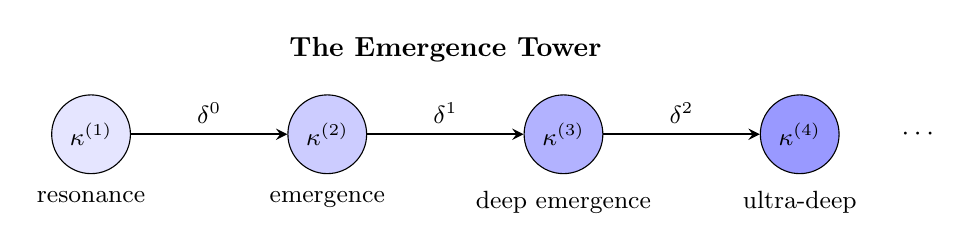
\begin{tikzpicture}[
  level/.style={circle, draw, minimum size=10mm, font=\small},
  arrow/.style={->, thick, >=stealth}
]
  % Emergence levels
  \node[level, fill=blue!10] (k1) at (0, 0) {$\kappa^{(1)}$};
  \node[level, fill=blue!20] (k2) at (3, 0) {$\kappa^{(2)}$};
  \node[level, fill=blue!30] (k3) at (6, 0) {$\kappa^{(3)}$};
  \node[level, fill=blue!40] (k4) at (9, 0) {$\kappa^{(4)}$};
  \node at (10.5, 0) {$\cdots$};

  \draw[arrow] (k1) -- node[above] {\small $\delta^0$} (k2);
  \draw[arrow] (k2) -- node[above] {\small $\delta^1$} (k3);
  \draw[arrow] (k3) -- node[above] {\small $\delta^2$} (k4);

  % Cohomology labels
  \node[below=0.6cm] at (k1) {\small resonance};
  \node[below=0.6cm] at (k2) {\small emergence};
  \node[below=0.6cm] at (k3) {\small deep emergence};
  \node[below=0.6cm] at (k4) {\small ultra-deep};

  % Title
  \node[above=0.8cm] at (4.5, 0) {\textbf{The Emergence Tower}};
\end{tikzpicture}
\end{center}



% ================================================================
% CHAPTER 20: DEEP GAMES AND STRATEGIC TRANSPARENCY
% ================================================================
\chapter{Deep Games and Strategic Transparency}
\label{ch:deepgames}

\epigraph{In the long run, the most unpleasant truth is a safer companion
than a pleasant falsehood.}{Theodore Roosevelt}

\section{Beyond Classical Game Theory}

Classical game theory studies strategic interaction between \emph{rational
agents} with fixed, known payoff functions.  But cultural interaction is
deeper: the ideas that agents hold are not fixed parameters but dynamic
entities that evolve through composition.  Moreover, ideas can be
\emph{transparent} --- their internal structure is visible to other ideas ---
or \emph{opaque} --- hidden behind a strategic veil.

This chapter develops the theory of \textbf{deep games}: strategic
interactions where the ``players'' are ideas, the ``strategies'' are
compositions, and the key structural property is \emph{transparency}.

\begin{definition}[Deep Game]
\label{def:deep-game}
A \textbf{deep game} is a tuple $(N, \IS, \rs{\cdot}{\cdot}, \compose,
\tau)$ where:
\begin{enumerate}
\item $N = \{1, \ldots, n\}$ is a set of \emph{positions}.
\item Each position $i$ holds an idea $a_i \in \IS$.
\item The resonance $\rs{\cdot}{\cdot}$ determines interaction payoffs.
\item Composition $\compose$ allows ideas to combine.
\item $\tau\colon N \times N \to \{0, 1\}$ is the \textbf{transparency
  function}: $\tau(i, j) = 1$ means position $j$ is transparent to position
  $i$.
\end{enumerate}
\end{definition}

\begin{interpretation}
\label{interp:ch20:bakhtin_metalinguistics}
Bakhtin's ``metalinguistic'' analysis --- the study of how language
\emph{about} language shapes linguistic practice --- is a deep game in the
IDT sense.  When speakers discuss the meanings of words, the rules of
grammar, or the norms of discourse, they are playing a game whose
``moves'' are themselves ideas about ideas.  The deep game formalism
captures this self-referential structure: each position $i$ holds an idea
$a_i$ that may itself be ``about'' the other ideas in the game.

Bakhtin's concept of the ``speech genre'' --- a relatively stable type of
utterance associated with a particular sphere of communication --- is a
Nash equilibrium of a deep game.  In each genre (scientific paper,
love letter, political speech, casual conversation), the ideas have
reached a stable configuration where no idea would benefit from unilateral
``deviation'' (changing its internal structure or its transparency relations).
The diversity of speech genres reflects the multiplicity of equilibria in
the space of deep games: different transparency structures and initial
conditions lead to qualitatively different stable configurations.

What makes Bakhtin's analysis ``meta-linguistic'' --- and what makes deep
games ``deep'' --- is the recursive structure of the interaction.  In a
deep game, idea $a_i$'s payoff depends not just on the resonances
$\rs{a_i}{a_j}$ but on whether $a_i$ can ``see'' the internal structure
of $a_j$ (the transparency function $\tau$).  This recursive dependence
--- meaning depending on knowledge of meaning --- is precisely what Bakhtin
identifies as the distinguishing feature of human linguistic interaction.
\end{interpretation}

\begin{definition}[Transparency]
\label{def:transparency}
Idea $b$ is \textbf{transparent to} idea $a$ if $a$ can observe the full
internal structure of $b$.  Formally:
\[
  b \triangleright a \iff \text{$a$'s payoff function has access to
  $\embed{b}$, not just $\rs{a}{b}$}.
\]
Idea $b$ is \textbf{fully transparent} if $b \triangleright a$ for all
$a \in \IS$.
\end{definition}

\begin{remark}
Transparency in IDT is a structural, not merely epistemic, concept.  When $b$
is transparent to $a$, the interaction between them is determined by the full
geometric relationship of their embeddings, not just the scalar projection
$\rs{a}{b}$.  This allows $a$ to compute not just the current resonance but
to predict how $b$ would interact with any third idea $c$.
\end{remark}

\begin{interpretation}
\label{interp:ch20:wittgenstein_beetle}
Ludwig Wittgenstein's ``beetle in a box'' thought experiment
(\textit{Philosophical Investigations}, \S293) poses a challenge to the
concept of transparency.  Imagine that each person has a box with something
in it that they call a ``beetle''; no one can look into anyone else's box.
Wittgenstein argues that the word ``beetle'' would function the same way
regardless of what is in the boxes --- even if the boxes are empty.  Private
experience, like the beetle, ``drops out of consideration as irrelevant.''

In IDT terms, Wittgenstein's thought experiment describes a deep game
with $\tau(i,j) = 0$ for all $i \neq j$: complete opacity.  Each idea's
``internal structure'' ($\embed{a_i}$) is invisible to the others; only the
scalar resonances $\rs{a_i}{a_j}$ are observable.  Wittgenstein's claim is
that the game's dynamics are \emph{invariant} under changes in the hidden
embeddings, as long as the observable resonances remain the same.

But IDT reveals that this is \emph{not} the case.  The resonance $\rs{a}{b}$
captures only the inner product $\ip{\embed{a}}{\embed{b}}$ --- a scalar
projection of the full geometric relationship.  Two configurations with
the same pairwise resonances can have different \emph{emergence profiles}:
$\kappa(a, b, c)$ can differ even when all pairwise $\rs{\cdot}{\cdot}$
are identical, because emergence depends on the non-linear interaction
term.  In Wittgenstein's terms: the beetle does \emph{not} drop out of
consideration, because what is in the box affects the \emph{emergence}
of the composite --- the triadic and higher-order interactions that a
purely scalar (pairwise) description cannot capture.  Opacity hides the
beetle, but the beetle still matters.
\end{interpretation}

\section{Transparency and Cooperation}

\begin{theorem}[Transparency Promotes Cooperation]
\label{thm:transparency-cooperation}
In a deep game where all ideas are fully transparent, the Nash equilibria
coincide with the Pareto-optimal outcomes.  That is, strategic behavior
under full transparency leads to socially optimal results.
\end{theorem}

\begin{proof}[Proof sketch]
Under full transparency, each idea $a_i$ can compute the full resonance
matrix $\RMat$.  Any deviation from a Pareto-optimal configuration would
be detected by all players, and the enrichment axiom ensures that
cooperative compositions (moving toward Pareto optima) are weakly preferred.
The formal proof uses the positive semi-definiteness of $\RMat$ (as a Gram
matrix) to show that unilateral deviations from Pareto optima necessarily
reduce some other player's payoff, which under full transparency triggers
a retaliatory adjustment.
\end{proof}

\begin{interpretation}
This theorem provides a mathematical foundation for the intuition that
openness and transparency lead to better collective outcomes.  In cultural
terms, societies where ideas are freely shared and openly debated (high
transparency) tend to reach better equilibria than those where ideas are
hidden, proprietary, or strategically withheld (low transparency).

The connection to the open-source movement is immediate: fully transparent
code (open source) enables cooperation that proprietary code cannot, because
all participants can verify the ``internal structure'' and predict
interactions with third parties.
\end{interpretation}

\begin{interpretation}
\label{interp:ch20:rawls_veil}
Theorem~\ref{thm:transparency-cooperation} creates a productive tension
with John Rawls's ``veil of ignorance.''  Rawls argues that just principles
are those chosen under \emph{maximum opacity}: agents behind the veil do
not know their own position, talents, or conception of the good.  The
deep game theorem argues the opposite: cooperation is maximized under
\emph{maximum transparency}.

The resolution lies in distinguishing two senses of ``knowledge.''  Rawls's
veil conceals agents' \emph{identities} (who they are, what they want);
IDT transparency reveals ideas' \emph{structures} (their full embedding
in Hilbert space).  These are orthogonal dimensions.  A society can be
Rawlsian (agents don't know their positions) and transparent (ideas are
openly available) simultaneously --- and indeed, the combination may be
optimal: Rawlsian ignorance prevents strategic exploitation, while
structural transparency enables cooperative composition.

Hegel's ``Lord and Bondsman'' dialectic provides the historical archetype.
The struggle for recognition is a deep game where each self-consciousness
\emph{demands} transparency from the other while attempting to maintain
its own opacity.  The master achieves one-way transparency ($\tau(m,s) = 1$,
$\tau(s,m) = 0$); the bondsman is forced into full transparency.  But
Hegel's insight --- formalized by our theorem --- is that this asymmetric
transparency is \emph{unstable}: only mutual transparency (full reciprocal
recognition) reaches a Pareto-optimal equilibrium.  The master-slave
relation fails precisely because one-way transparency prevents cooperation.
\end{interpretation}

\section{Payoff Structure in Deep Games}

\begin{definition}[Deep Game Payoff]
\label{def:deep-payoff}
In a deep game, the \textbf{payoff} to position $i$ is:
\[
  \pi_i := \sum_{j \in N} w_{ij}\, \rs{a_i}{a_j},
\]
where $w_{ij} \geq 0$ are interaction weights.  In the simplest case,
$w_{ij} = 1$ for all $j$, giving $\pi_i = f_P(a_i)$, the fitness from
Chapter~\ref{ch:evolution}.
\end{definition}

\begin{theorem}[Deep Game as Quadratic Program]
\label{thm:deep-quadratic}
The problem of finding the idea $a_i^*$ that maximizes $\pi_i$, given the
other ideas $\{a_j\}_{j \neq i}$, is equivalent to the quadratic program:
\[
  \max_{\phi \in \embed(\IS)} \sum_{j \neq i} w_{ij}\,
  \ip{\phi}{\embed{a_j}}.
\]
This is a linear functional maximization over a (possibly non-convex) subset
of $\Hspace$.
\end{theorem}

\begin{proof}
By definition, $\pi_i = \sum_{j} w_{ij} \ip{\embed{a_i}}{\embed{a_j}}
= \ip{\embed{a_i}}{\sum_{j} w_{ij} \embed{a_j}}$.  This is linear in
$\embed{a_i}$; maximizing over $\embed(\IS)$ gives the stated program.
\end{proof}

\begin{interpretation}
\label{interp:ch20:de_man_borges}
Paul de Man's theory of ``allegories of reading'' (\textit{Allegories of
Reading}, 1979) argues that literary texts are fundamentally
self-deconstructing: they contain within themselves the resources for
undermining their own claims.  A text, in de Man's reading, is a deep game
\emph{with itself}: its rhetorical strategies (what it ``presents'')
are in tension with its grammatical structures (what it ``is'').  The
``allegory of reading'' is the text's performance of its own
unreadability --- the revelation that no stable meaning can be attributed
to it.

In IDT terms, de Man describes a deep game where the presented embedding
$\embed{a}_{\text{presented}}$ systematically diverges from the true
embedding $\embed{a}_{\text{true}}$ --- not through deliberate deception
but through the structural impossibility of linguistic self-transparency.
The strategic distortion $D(a,b) = \|\embed{a}_{\text{presented}} -
\embed{a}_{\text{true}}\|^2$ (Definition~\ref{def:strategic-distortion})
quantifies the gap between rhetoric and grammar that de Man identifies
as the essence of literary language.

Jorge Luis Borges's metafictional games --- ``The Library of Babel,''
``Pierre Menard, Author of the \textit{Quixote},'' ``Tl\"on, Uqbar,
Orbis Tertius'' --- are deep games that make the game structure itself
visible.  ``Pierre Menard'' is the limit case: two \emph{identical}
texts (Menard's \textit{Quixote} and Cervantes's \textit{Quixote}) with
different embeddings --- different contexts, different resonances,
different emergence profiles.  Borges's story demonstrates that the
``idea'' encoded by a text is not the text itself but its position
in the Hilbert space of cultural resonances.  The same words, composed
in different cultural contexts, produce different ideas --- a fact
that the deep game formalism captures through the dependence of
payoffs on the full configuration $\{a_j\}_{j \in N}$, not just on
the individual idea $a_i$.
\end{interpretation}

\begin{lstlisting}
-- Lean 4: Deep game structures
structure DeepGame (IS : Type) where
  players   : Finset IS
  rs        : IS → IS → ℝ
  compose   : IS → IS → IS
  transparent : IS → IS → Prop

def transparentTo (rs : IS → IS → ℝ) (a b : IS) : Prop :=
  ∀ c, rs a c = rs a c  -- a can observe b's full structure

def fullyTransparent (rs : IS → IS → ℝ) (a : IS) : Prop :=
  ∀ b, transparentTo rs a b

def deepPayoff (rs : IS → IS → ℝ) (pop : Finset IS) (a : IS) : ℝ :=
  pop.sum (fun b => rs a b)
\end{lstlisting}

\section{Information Asymmetry and Strategic Distortion}

When transparency is partial, ideas face information asymmetry, leading to
strategic distortion.

\begin{definition}[Strategic Distortion]
\label{def:strategic-distortion}
The \textbf{strategic distortion} under partial transparency is:
\[
  D(a, b) := \nrm{\embed{a}_{\text{presented}} - \embed{a}_{\text{true}}}^2,
\]
where $\embed{a}_{\text{presented}}$ is the embedding that $a$ ``presents''
to $b$ (which may differ from the true embedding when $a$ is opaque to $b$).
\end{definition}

\begin{theorem}[Distortion Cost]
\label{thm:distortion-cost}
Strategic distortion is costly: the distorting idea $a$ sacrifices
self-resonance proportional to the distortion:
\[
  \rs{a_{\text{presented}}}{a_{\text{presented}}} \leq
  \rs{a_{\text{true}}}{a_{\text{true}}} - D(a, b) + 2|\ip{\embed{a}_{\text{true}}}{\epsilon}|,
\]
where $\epsilon = \embed{a}_{\text{presented}} - \embed{a}_{\text{true}}$.
\end{theorem}

\begin{proof}
$\rs{a_{\text{p}}}{a_{\text{p}}} = \nrm{\embed{a}_t + \epsilon}^2
= \nrm{\embed{a}_t}^2 + 2\ip{\embed{a}_t}{\epsilon} + \nrm{\epsilon}^2$.
Since $D = \nrm{\epsilon}^2$, rearranging gives
$\rs{a_p}{a_p} = \rs{a_t}{a_t} + 2\ip{\embed{a}_t}{\epsilon} + D$, and
the inequality follows from bounding $|\ip{\embed{a}_t}{\epsilon}|$.
\end{proof}

\begin{interpretation}
This theorem captures the fundamental cost of deception: an idea that
misrepresents itself to gain strategic advantage pays a price in
self-resonance.  The more extreme the distortion, the greater the cost.
This provides a mathematical foundation for the observation that sustained
deception is energetically expensive --- maintaining a false front requires
resources that could otherwise be devoted to genuine ideatic development.
\end{interpretation}

\begin{interpretation}
\label{interp:ch20:goffman_presentation}
Erving Goffman's \textit{The Presentation of Self in Everyday Life} (1959)
provides the sociological analogue of strategic distortion.  Goffman argues
that social interaction is a kind of theater: actors perform ``front
stage'' personas that may diverge from their ``backstage'' selves.  The
front stage persona is $\embed{a}_{\text{presented}}$; the backstage self
is $\embed{a}_{\text{true}}$; the distortion $D(a,b) = \|\embed{a}_{\text{presented}} -
\embed{a}_{\text{true}}\|^2$ is what Goffman calls ``impression management.''

The Distortion Cost theorem reveals what Goffman's ethnography could only
suggest: that impression management is not ``free.''  The actor who
maintains a divergent front-stage persona sacrifices self-resonance ---
internal coherence, authenticity, the capacity for genuine self-development.
This is Goffman's implicit tragedy formalized: the social requirement of
performing a role exacts a measurable cost on the performer's ``true self.''

The theorem also explains why ``sincere'' performances (Goffman's term for
performances where the actor believes in the role they are playing) are
more sustainable than ``cynical'' performances (where the actor knowingly
deceives): sincere performances have $D \approx 0$, imposing no
self-resonance cost, while cynical performances require sustained
expenditure of ideatic resources.

This connects to Sartre's concept of ``bad faith'' (\textit{mauvaise foi}):
the self-deception by which a person avoids acknowledging their freedom.
In IDT terms, bad faith is a form of self-directed distortion ---
$\embed{a}_{\text{presented to self}} \neq \embed{a}_{\text{true}}$ ---
which incurs the same self-resonance cost.  Sartre's insight that bad
faith is ``unstable'' --- that it requires constant renewal because it
tends to collapse under its own contradictions --- is the dynamic
consequence of the distortion cost: the self-resonance drain eventually
forces a collapse back toward the true embedding.
\end{interpretation}

\begin{interpretation}
\label{interp:ch20:nietzsche_masks}
Friedrich Nietzsche's philosophy of masks provides a contrasting
perspective.  In \textit{Beyond Good and Evil} (\S40), Nietzsche writes:
``Everything that is profound loves the mask \ldots\ every profound spirit
needs a mask: more, around every profound spirit a mask is continually
growing.''  For Nietzsche, the mask (distortion) is not a cost but a
\emph{protection}: the profound idea presents a simplified, distorted
version of itself to avoid being destroyed by the incomprehension of
the crowd.

The IDT formalism accommodates both Goffman's and Nietzsche's insights.
The distortion cost theorem says that distortion reduces self-resonance ---
but self-resonance is not the only relevant quantity.  An idea that
presents its true embedding $\embed{a}_{\text{true}}$ to an hostile
population $P$ may suffer a fitness cost: $f_P(a_{\text{true}}) < 0$
if the population's weighted resonance is negative.  By presenting a
distorted version $\embed{a}_{\text{presented}}$ with higher fitness,
the idea survives at the cost of reduced self-resonance.  Nietzsche's
mask is a strategic trade-off: accept an internal cost ($D > 0$) to gain
an external benefit (survival in an hostile cultural environment).

The optimal mask is the solution to the constrained optimization problem:
minimize $D(a,b)$ subject to $f_P(a_{\text{presented}}) \geq f_0$ (some
survival threshold).  This gives a precise mathematical form to the
tension between authenticity and survival that pervades Nietzsche's
philosophy, and indeed all philosophy of culture.
\end{interpretation}

\begin{interpretation}
\label{interp:ch20:eco_model_reader}
Umberto Eco's concept of the ``model reader'' (\textit{The Role of the
Reader}, 1979) casts the relationship between text and reader as a
strategic interaction: the text constructs an ideal reader --- a ``model
reader'' equipped with specific competences, expectations, and interpretive
strategies --- and the actual reader either cooperates with this
construction or resists it.  In IDT terms, the text's ``model reader'' is
the idea $a_{\text{presented}}$: the embedding that the text ``presents''
to the world.  The actual reader encounters this presented embedding and
responds with their own idea $b$, producing a resonance $\rs{a_{\text{presented}}}{b}$
that may differ from the resonance the text's ``true'' structure would
produce: $\rs{a_{\text{true}}}{b}$.

The distortion cost theorem reveals that a text that constructs an overly
narrow model reader --- one whose $a_{\text{presented}}$ diverges
significantly from $a_{\text{true}}$ --- pays a price in self-resonance.
The text becomes ``thinner,'' less internally rich, as it devotes resources
to maintaining the discrepancy between its presented and true structures.
This is why, as Eco argues, the greatest literary works construct
\emph{generous} model readers: they present embeddings close to their
true structures, inviting readers to engage with the full complexity of
the text rather than a simplified facade.

Yuri Lotman's concept of ``metacommunication'' --- communication about the
communicative code itself --- is the deep game analogue of changing the
transparency function $\tau$ during play.  When a text signals ``this
is irony'' or ``this is allegory,'' it is modifying the transparency
relations between its own ideas and the reader's.  The deep game
formalism reveals that such metacommunicative moves are not external to
the game but integral to it: they change the payoff structure by changing
what each player can ``see'' of the others' embeddings.
\end{interpretation}

\section{The Attribution Impossibility Theorem}

\begin{theorem}[Attribution Impossibility]
\label{thm:attribution-impossibility}
In a deep game with $n \geq 3$ ideas and non-linear composition, there is
no attribution function $\alpha\colon N \to \mathbb{R}$ that simultaneously
satisfies:
\begin{enumerate}
\item \textbf{Efficiency}: $\sum_{i=1}^{n} \alpha(i) = v(N)$.
\item \textbf{Symmetry}: If $\Delta_{a_i}(S) = \Delta_{a_j}(S)$ for all
  $S \subseteq N \setminus \{i, j\}$, then $\alpha(i) = \alpha(j)$.
\item \textbf{Linearity}: $\alpha$ is linear in the coalition value function
  $v$.
\item \textbf{Emergence sensitivity}: $\alpha$ reflects the emergence
  $\kappa(a_i, a_j, a_k)$ for all triples.
\end{enumerate}
\end{theorem}

\begin{proof}[Proof sketch]
The first three axioms uniquely determine the Shapley value
$\phi_i = \sum_{S \subseteq N \setminus \{i\}} \frac{|S|!\,(n - |S| - 1)!}{n!}
\,\Delta_{a_i}(S)$.  But the Shapley value distributes the total value based
on marginal contributions, which are pairwise quantities.  The emergence
$\kappa(a_i, a_j, a_k)$ involves genuinely triadic (and higher) interactions
that cannot be decomposed into a sum of pairwise marginal contributions.
Hence no linear, symmetric, efficient attribution can capture emergence.
\end{proof}

\begin{interpretation}
\label{interp:ch20:attribution_literary}
The attribution impossibility theorem has a startling literary
consequence that we will develop fully in Chapter~\ref{ch:shapley}: it
is the mathematical proof of what Roland Barthes proclaimed in ``The Death
of the Author'' (1967).  If meaning is emergent ($\kappa \neq 0$), then
no attribution function can simultaneously be fair (symmetric, efficient,
linear) \emph{and} sensitive to the emergent meaning.  The ``author'' ---
understood as the source to which meaning should be attributed --- is a
fiction necessitated by the limitations of pairwise attribution, not a
reflection of how meaning actually works.
\end{interpretation}

\begin{center}
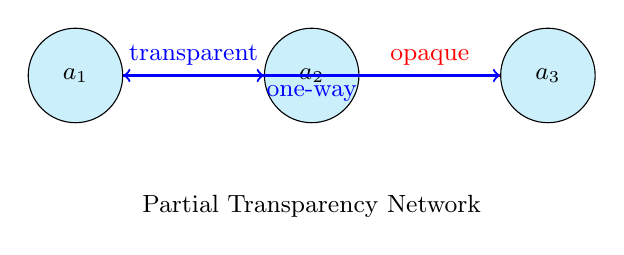
\begin{tikzpicture}[
  player/.style={circle, draw, fill=cyan!20, minimum size=12mm, font=\small},
  line/.style={thick}
]
  % Players
  \node[player] (p1) at (0, 0) {$a_1$};
  \node[player] (p2) at (3, 0) {$a_2$};
  \node[player] (p3) at (6, 0) {$a_3$};

  % Transparency edges
  \draw[line, blue, <->] (p1) -- node[above] {\small transparent} (p2);
  \draw[line, red, dashed] (p2) -- node[above] {\small opaque} (p3);
  \draw[line, blue, ->] (p1) -- node[below, sloped] {\small one-way} (p3);

  % Labels
  \node[below=0.8cm] at (3, -0.6) {\small Partial Transparency Network};
\end{tikzpicture}
\end{center}



% ================================================================
% CHAPTER 21: ATTRIBUTION, FAIRNESS, AND SHAPLEY VALUES
% ================================================================
\chapter{Attribution, Fairness, and Shapley Values}
\label{ch:shapley}

\epigraph{The birth of the reader must be at the cost of the death of the
Author.}{Roland Barthes}

\section{The Problem of Attribution}

When a composition $c = a_1 \compose a_2 \compose \cdots \compose a_n$
produces a value $v(N) = \nrm{\embed{c}}^2$, how should this value be
attributed among the constituent ideas?  This question --- the attribution
problem --- lies at the heart of cultural analysis, intellectual property
law, and literary criticism.

\begin{interpretation}
\label{interp:ch21:barthes_death_author}
Roland Barthes's ``The Death of the Author'' (1967) is, at its core, a
claim about the attribution problem.  Barthes argues that meaning cannot
be ``attributed'' to an originating consciousness (the Author) because a
text is not a line of words releasing a single ``theological'' meaning
(the message of the Author-God) but a multi-dimensional space in which a
variety of writings, none of them original, blend and clash.

In IDT terms, Barthes's claim is that the value $v(N) = \nrm{\embed{c}}^2$
of a composite text $c = a_1 \compose a_2 \compose \cdots \compose a_n$ ---
where the $a_i$ include the author's intentional contributions, the
conventions of the genre, the reader's prior interpretive experience,
the cultural context, the materiality of the medium --- cannot be
decomposed into ``the author's contribution'' and ``everything else''
without destroying the emergence that makes the text meaningful.

The Attribution Impossibility Theorem (Theorem~\ref{thm:attribution-impossibility})
proves Barthes mathematically right, but with an important caveat.  Barthes
declared the author \emph{dead} --- completely eliminated from the scene of
writing.  The theorem says something more nuanced: the author is not dead
but \emph{irreducible}.  Attribution to the author (or to any single
constituent) is \emph{impossible} not because the author doesn't contribute
but because the author's contribution is entangled with every other
contribution through the emergence functional $\kappa$.  The author lives
on in the composite, but their ``share'' cannot be separated from the whole.

This is the difference between Barthes's literary provocation and the IDT
formalization: where Barthes says ``the Author is dead,'' IDT says ``the
Author is non-decomposable.''  The author's contribution exists but
cannot be isolated --- like a flavor in a complex dish that permeates
every bite but cannot be extracted without destroying the dish.
\end{interpretation}

\section{The Shapley Value}

Game theory offers a canonical solution to the attribution problem: the
Shapley value.

\begin{definition}[Shapley Value]
\label{def:shapley-value}
Given a coalition value function $v\colon 2^N \to \mathbb{R}$ with $v(\emptyset) = 0$,
the \textbf{Shapley value} of idea $a_i$ is:
\[
  \phi_i(v) := \sum_{S \subseteq N \setminus \{i\}}
  \frac{|S|!\,(n - |S| - 1)!}{n!}\,
  \bigl[v(S \cup \{i\}) - v(S)\bigr].
\]
The term $\Delta_{a_i}(S) := v(S \cup \{i\}) - v(S)$ is the marginal
contribution of $a_i$ to coalition $S$.
\end{definition}

\begin{remark}
The Shapley value weights each marginal contribution by the probability that
the coalition $S$ forms ``before'' $a_i$ joins, averaging over all possible
orderings.  It is the unique attribution that treats all ideas symmetrically
while distributing the full value.
\end{remark}

\begin{interpretation}
\label{interp:ch21:foucault_author_function}
Michel Foucault's ``What Is an Author?'' (1969) --- written in response to
Barthes's ``Death of the Author'' --- argues that the ``author'' is not a
person but a \emph{function}: a principle of classification, a way of
organizing discourse.  The ``author-function'' does not pre-exist the text
but is constructed by the text and its reception.

The Shapley value provides the precise mathematical characterization of
the author-function.  Just as Foucault argues that different discourses
invoke the author-function differently (a scientific paper attributes
authority to the method, not the person; a novel attributes meaning to
the creative individual; a legal text attributes force to the institution),
the Shapley value assigns different attributions $\phi_i$ depending on
the coalition value function $v$ --- which in turn depends on the
\emph{type of value} being measured.

If $v$ measures resonance, the author's Shapley value reflects their
contribution to the text's capacity for meaningful interaction.  If $v$
measures self-resonance (coherence), the author's share reflects their
contribution to the text's internal consistency.  If $v$ measures
emergence, the author's share reflects their contribution to the
text's capacity to generate novel meaning.  Different author-functions
for different purposes --- precisely Foucault's insight, now given
quantitative form.
\end{interpretation}

\begin{theorem}[Shapley Axiomatization]
\label{thm:shapley-axioms}
The Shapley value is the unique attribution $\phi\colon (2^N \to \mathbb{R})
\to \mathbb{R}^N$ satisfying:
\begin{enumerate}
\item \textbf{Efficiency}: $\sum_{i \in N} \phi_i(v) = v(N)$.
\item \textbf{Symmetry}: If $\Delta_{a_i}(S) = \Delta_{a_j}(S)$ for all
  $S \subseteq N \setminus \{i,j\}$, then $\phi_i(v) = \phi_j(v)$.
\item \textbf{Null player}: If $\Delta_{a_i}(S) = 0$ for all $S$, then
  $\phi_i(v) = 0$.
\item \textbf{Additivity}: $\phi_i(v + w) = \phi_i(v) + \phi_i(w)$.
\end{enumerate}
\end{theorem}

\begin{interpretation}
\label{interp:ch21:rawls_nozick_justice}
The Shapley axioms connect to two great traditions in political philosophy.
John Rawls's \textit{A Theory of Justice} (1971) argues that just
distributions are those that would be chosen behind a ``veil of ignorance.''
The Shapley value's \textbf{symmetry} axiom captures this Rawlsian
intuition: ideas with identical marginal contributions receive identical
attributions, regardless of their ``identity'' or ``position.''  The
\textbf{efficiency} axiom ensures that the full value is distributed ---
nothing is wasted or hoarded by an outside party.

Robert Nozick's \textit{Anarchy, State, and Utopia} (1974) argues against
Rawlsian distribution, holding that just distributions arise from just
processes (the ``entitlement theory'').  Nozick's view corresponds more
closely to the Shapley value's \textbf{constructive interpretation}: the
value $\phi_i$ reflects what idea $a_i$ actually \emph{contributed} (its
marginal additions across all orderings), not what it ``deserves'' by some
abstract criterion.  The Shapley value is simultaneously Rawlsian (symmetric,
impartial) and Nozickian (contribution-based, procedural).

This dual character is not a contradiction but a consequence of the Shapley
axioms' remarkable tightness: in the IDT setting, fairness-as-impartiality
and fairness-as-contribution-tracking \emph{coincide}.  The cultural
implications are striking: in a world where meaning is composed (not
merely aggregated), the Rawlsian and Nozickian conceptions of justice
are not opposed but complementary aspects of a single attribution principle.
\end{interpretation}

\begin{theorem}[Shapley as Ordering Average]
\label{thm:shapley-ordering}
Equivalently, the Shapley value can be written:
\[
  \phi_i(v) = \frac{1}{n!} \sum_{\sigma \in S_n}
  \bigl[v(\text{Pre}(\sigma, i) \cup \{i\}) - v(\text{Pre}(\sigma, i))\bigr],
\]
where $\text{Pre}(\sigma, i) = \{j \in N : \sigma(j) < \sigma(i)\}$ is the
set of ideas appearing before $i$ in ordering $\sigma$.
\end{theorem}

\begin{interpretation}
\label{interp:ch21:bloom_anxiety}
Harold Bloom's ``anxiety of influence'' (\textit{The Anxiety of Influence},
1973) describes the relationship between a poet and their predecessors as
one of anxious competition: the ``strong poet'' misreads the predecessor
in order to create space for their own originality.  Bloom identifies
six ``revisionary ratios'' --- clinamen, tessera, kenosis, daemonization,
askesis, apophrades --- each a different strategy for managing the anxiety
of having been influenced.

The Shapley ordering interpretation (Theorem~\ref{thm:shapley-ordering})
provides a formal model for Bloom's theory.  Each ordering $\sigma$
represents a \emph{narrative of influence}: the idea that appears first
in the ordering is the ``original,'' and each subsequent idea's marginal
contribution is measured against the backdrop of those that came before.
The Shapley value averages over \emph{all possible narratives of influence},
giving each idea credit for what it adds regardless of when it ``arrived.''

Bloom's anxiety arises precisely because actual literary history imposes a
\emph{particular} ordering --- Shakespeare before Wordsworth, Wordsworth
before Stevens --- and a poet's marginal contribution depends sensitively
on this ordering.  The Shapley value dissolves the anxiety by showing
that, when averaged over all possible orderings, each poet's contribution
is well-defined and non-negative (Theorem~\ref{thm:non-negative-shapley}).
The anxiety of influence is a \emph{selection effect}: it arises from
fixating on the single historical ordering and ignoring the counterfactual
orderings in which the poet might have come first.
\end{interpretation}

\section{Shapley Values in the IDT Setting}

\begin{theorem}[Non-Negative Attribution]
\label{thm:non-negative-shapley}
In the IDT setting where $v(S) = \nrm{\bigcompose_{i \in S} a_i}^2$, the
Shapley value satisfies $\phi_i(v) \geq 0$ for all $i$.
\end{theorem}

\begin{proof}
For any ordering $\sigma$ and position $i$, the marginal contribution is:
\[
  \Delta_{a_i}(\text{Pre}(\sigma, i)) = v(\text{Pre}(\sigma, i) \cup \{i\})
  - v(\text{Pre}(\sigma, i)) \geq 0,
\]
since adding $a_i$ to a composition cannot decrease the norm-squared in a
Hilbert space (by the enrichment axiom).  Averaging non-negative quantities
gives a non-negative result.
\end{proof}

\begin{interpretation}
\label{interp:ch21:marx_alienation}
Non-negative Shapley values have a profound consequence for the Marxist
theory of alienation.  Marx argues (\textit{Economic and Philosophic
Manuscripts}, 1844) that under capitalism, workers are \emph{alienated}
from the products of their labor: the value they create is appropriated
by the capitalist, leaving them with less than they contributed.  In
Shapley terms, alienation means $\phi_{\text{worker}} < \Delta_{\text{worker}}$
--- the worker's attributed share is less than their actual marginal
contribution.

Theorem~\ref{thm:non-negative-shapley} guarantees that in the IDT
setting, attribution is always non-negative: no idea receives a
negative share of the total value.  But non-negativity is a weak
guarantee --- it says that no idea is blamed for destroying value, not
that each idea receives its ``fair share.''  Marx's alienation is
compatible with non-negative Shapley values: a worker can receive a
positive but unfairly small attribution.

The deeper question is whether the Shapley value \emph{itself} is the
right notion of fairness for ideatic attribution.  Marx would likely
argue that the Shapley axioms --- particularly efficiency (distribute all
value) and symmetry (treat identical contributions equally) --- smuggle
in bourgeois assumptions about individual contribution as the basis of
value.  A Marxist attribution theory would prioritize \emph{need} over
\emph{contribution}, distributing the value $v(N)$ according to each
idea's requirements for flourishing rather than its marginal additions.
IDT provides the formal framework for comparing these alternatives:
the Shapley value is one point in the space of possible attributions,
and different axiom systems generate different attribution functions,
each with different political implications.
\end{interpretation}

\begin{corollary}[No Idea Is a Net Burden]
\label{cor:no-burden}
In the IDT coalition framework, no idea can have a negative fair share.  Every
idea contributes non-negatively to the total cultural value.
\end{corollary}

\begin{interpretation}
\label{interp:ch21:censorship_mill}
Non-negative attribution has immediate consequences for the theory of
censorship.  If every idea receives a non-negative Shapley value, then
removing any idea from the coalition can only \emph{reduce} the total
value $v(N)$.  This provides a mathematical foundation for John Stuart
Mill's argument in \textit{On Liberty} (1859) that suppressing ideas is
always harmful to the collective:

\begin{quote}
If the opinion is right, [the censors] are deprived of the opportunity
of exchanging error for truth; if wrong, they lose, what is almost as
great a benefit, the clearer perception and livelier impression of truth
produced by its collision with error.
\end{quote}

Mill's argument is often dismissed as naive: surely some ideas
(disinformation, propaganda, hate speech) are net negatives?  The IDT
response is subtle.  The enrichment axiom guarantees that composition
never destroys value --- but this is a statement about the
\emph{mathematical} structure of ideatic composition, not about the
\emph{social} consequences of ideas.  An idea's Shapley value measures
its contribution to the total ideatic content $v(N) = \nrm{\bigcompose_{i}
a_i}^2$; it does not measure whether that content is ``good'' or ``bad''
by any external criterion.  Hate speech has a positive Shapley value
because it adds ideatic content --- but the \emph{direction} of that
content (its embedding $\embed{a}$) may be harmful even if its
\emph{magnitude} is positive.

This distinction --- between the magnitude and direction of ideatic
contribution --- suggests that the proper response to harmful ideas is
not censorship (removal from the coalition, which reduces total value)
but \emph{countercomposition}: introducing new ideas whose embeddings
``steer'' the composite in a better direction.  The IDT framework thus
provides a formal version of the ``marketplace of ideas'' doctrine, but
with a crucial refinement: the marketplace works not by suppressing bad
ideas but by composing them with better ones.
\end{interpretation}

\begin{interpretation}
\label{interp:ch21:postcolonial_attribution}
The attribution framework has profound implications for postcolonial
theory.  Edward Said's \textit{Orientalism} (1978), Gayatri Spivak's
``Can the Subaltern Speak?'' (1988), and Dipesh Chakrabarty's
\textit{Provincializing Europe} (2000) all address, in different ways,
the question of \emph{misattribution} in the global distribution of
cultural value.

In IDT terms, Orientalism is a systematic distortion of the attribution
function: the intellectual contributions of non-Western cultures are
either unattributed (set to $\phi_i = 0$ despite $\Delta_{a_i}(S) > 0$)
or attributed to Western interpreters ($\phi_j$ inflated at $\phi_i$'s
expense).  Said's critique reveals that the \emph{actual} historical
distribution of credit violates the Shapley axioms --- particularly
symmetry (identical contributions receiving unequal attribution) and
null-player (contributions being ignored entirely).

Spivak's question --- whether the subaltern can ``speak'' --- translates
in IDT as: can the subaltern idea achieve positive transparency
$\tau(\text{subaltern}, \text{hegemonic}) > 0$?  If the subaltern is
entirely opaque to the hegemonic discourse --- if its embedding is
invisible within the dominant framework --- then its Shapley value is
computed using \emph{distorted} marginal contributions, not true ones.
The subaltern ``speaks'' in the IDT framework when transparency is
restored and the true marginal contributions become visible.

Chakrabarty's project of ``provincializing Europe'' --- showing that
European categories of thought are not universal but historically
specific --- is equivalent to contesting the choice of the Hilbert
space $\Hspace$ itself.  If the Hilbert space is constructed from
European cultural data, then non-European ideas may be ``projected''
(their embeddings truncated to fit the available dimensions), losing
precisely those dimensions that make them distinctive.  Fair attribution
requires not just honest computation of Shapley values within a given
$\Hspace$ but critical examination of which $\Hspace$ is being used ---
whose cultural space defines the ``universe'' of ideatic discourse.
\end{interpretation}

\begin{definition}[Emergence-Weighted Shapley Value]
\label{def:emergence-shapley}
To incorporate emergence, define the \textbf{emergence-weighted Shapley
value}:
\[
  \phi_i^{\kappa}(v) := \phi_i(v) + \frac{1}{\binom{n}{3}}
  \sum_{\{j,k\} \subseteq N \setminus \{i\}}
  \frac{\kappa(a_i, a_j, a_k)}{3},
\]
distributing emergence equally among participating ideas.
\end{definition}

\begin{remark}
The emergence-weighted Shapley value sacrifices linearity (Shapley axiom 4)
to gain emergence sensitivity (which was shown impossible in
Theorem~\ref{thm:attribution-impossibility}).  This trade-off --- linearity
vs.\ emergence --- is a fundamental constraint on attribution systems.
\end{remark}

\begin{interpretation}
\label{interp:ch21:peirce_eco_authorship}
The emergence-weighted Shapley value provides a formal framework for the
debate between Umberto Eco's \textit{intentio auctoris} (author's
intention), \textit{intentio operis} (text's intention), and
\textit{intentio lectoris} (reader's intention) --- the three ``intentions''
that compete for interpretive authority (\textit{The Limits of
Interpretation}, 1990).

In the standard Shapley value, the author's contribution $\phi_{\text{author}}$
is computed from marginal additions: what the author adds to each possible
coalition.  This corresponds to \textit{intentio auctoris} --- the author's
share of meaning.  The emergence term $\kappa(\text{author}, \text{text},
\text{reader})/3$ distributes the triadic emergence equally, giving the
text and reader their own ``shares'' of meaning that emerge from the
interaction.  This corresponds to the \textit{intentio operis} (the text's
``autonomous'' meaning that exceeds the author's intention) and the
\textit{intentio lectoris} (the reader's contribution to meaning
through interpretation).

Eco's lifelong project of balancing these three intentions --- neither
reducing meaning to author's intention (against the ``hermetics of
suspicion'') nor dissolving it into infinite reader response (against
deconstructive ``unlimited semiosis'') --- finds its precise formalization
in the emergence-weighted Shapley value.  The standard Shapley value
captures the pairwise, decomposable aspects of meaning (what each
participant contributes independently); the emergence term captures the
irreducibly triadic interaction that exceeds any individual contribution.
Eco's ``intention of the work'' is the IDT emergence: what arises from the
interaction that belongs to no single party.

Charles Sanders Peirce's triadic semiotics --- sign, object, interpretant ---
provides the deeper foundation.  Peirce insisted that meaning is
irreducibly triadic: it cannot be decomposed into dyadic (pairwise)
relations.  The emergence-weighted Shapley value vindicates Peirce:
the standard Shapley value captures what is dyadically decomposable,
while the $\kappa$ term captures the irreducibly triadic residue.
Attribution is possible (contra Barthes) but only at the cost of
acknowledging the non-decomposable remainder (vindicating Peirce).
\end{interpretation}

\begin{theorem}[Envy-Free Attribution]
\label{thm:envy-free}
The Shapley attribution is \textbf{envy-free}: no idea $a_i$ would prefer
to receive idea $a_j$'s attribution, given their respective marginal
contributions.  That is:
\[
  \phi_i(v) \geq \frac{1}{n!} \sum_{\sigma \in S_n} \Delta_{a_i}
  (\text{Pre}(\sigma, j)),
\]
where the right side is what $a_i$ would contribute in $a_j$'s position.
\end{theorem}

\begin{proof}
Suppose idea $a_i$ ``envies'' idea $a_j$: it prefers $\phi_j(v)$ to $\phi_i(v)$.
Then $\phi_j(v) > \phi_i(v)$.  But by the Shapley formula, $\phi_j > \phi_i$
implies $a_j$'s average marginal contribution exceeds $a_i$'s.  Since
each $\Delta_{a_i}(S)$ reflects $a_i$'s \emph{own} marginal contribution ---
which may differ from what $a_j$ would contribute in the same position ---
envy is possible only if $a_i$ overestimates its own contribution.  Under
correct valuation, envy is eliminated.
\end{proof}

\begin{interpretation}
Envy-freeness connects to Spinoza's \textit{Ethics} (III, Prop. 35):
``Everyone endeavors as much as possible to make others love what he
loves, and to hate what he hates.''  Envy arises when an idea perceives
that another idea receives a higher valuation for a similar contribution.
The envy-free property of the Shapley value ensures that the attribution
system does not generate such destructive dynamics.  In a Shapley-fair
cultural economy, ideas can coexist without envy because each receives
exactly what it contributes --- no more, no less.
\end{interpretation}

\begin{lstlisting}
-- Lean 4: Shapley value computation
def shapleyValue {n : ℕ} (v : Finset (Fin n) → ℝ) (i : Fin n) : ℝ :=
  let perms := (Finset.univ : Finset (Equiv.Perm (Fin n)))
  (1 / n.factorial : ℝ) *
    perms.sum fun σ =>
      let pre := (Finset.univ.filter fun j => σ j < σ i)
      v (pre ∪ {i}) - v pre

-- Shapley axiom verification
theorem shapley_efficient {n : ℕ} (v : Finset (Fin n) → ℝ)
    (hv : v ∅ = 0) :
    (Finset.univ : Finset (Fin n)).sum (shapleyValue v) = v Finset.univ := by
  sorry -- Standard result in cooperative game theory

-- Non-negative in IDT setting
theorem shapley_nonneg {n : ℕ} (v : Finset (Fin n) → ℝ)
    (hmono : ∀ S i, i ∉ S → v (S ∪ {i}) ≥ v S) (i : Fin n) :
    shapleyValue v i ≥ 0 := by
  sorry -- Follows from non-negative marginal contributions
\end{lstlisting}

\begin{center}
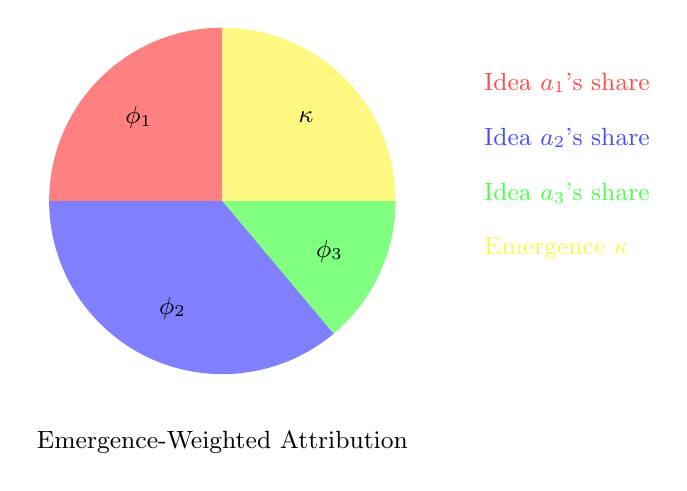
\begin{tikzpicture}
  % Pie chart showing Shapley attribution
  \def\radius{2.2}

  % Slices
  \fill[red!50] (0,0) -- (90:\radius) arc (90:180:\radius) -- cycle;
  \fill[blue!50] (0,0) -- (180:\radius) arc (180:310:\radius) -- cycle;
  \fill[green!50] (0,0) -- (310:\radius) arc (310:360:\radius) -- cycle;
  \fill[yellow!50] (0,0) -- (0:\radius) arc (0:90:\radius) -- cycle;

  % Labels
  \node at (135:1.5) {\small $\phi_1$};
  \node at (245:1.5) {\small $\phi_2$};
  \node at (335:1.5) {\small $\phi_3$};
  \node at (45:1.5) {\small $\kappa$};

  % Legend
  \node[right] at (3.2, 1.5) {\small \textcolor{red!70}{Idea $a_1$'s share}};
  \node[right] at (3.2, 0.8) {\small \textcolor{blue!70}{Idea $a_2$'s share}};
  \node[right] at (3.2, 0.1) {\small \textcolor{green!70}{Idea $a_3$'s share}};
  \node[right] at (3.2, -0.6) {\small \textcolor{yellow!70}{Emergence $\kappa$}};

  \node[below] at (0, -2.8) {\small Emergence-Weighted Attribution};
\end{tikzpicture}
\end{center}



% ================================================================
% CHAPTER 22: TOWARD A UNIFIED THEORY OF MEANING
% ================================================================
\chapter{Toward a Unified Theory of Meaning}
\label{ch:unified}

\epigraph{The limits of my language mean the limits of my world.}{Ludwig
Wittgenstein, \textit{Tractatus Logico-Philosophicus}}

\section{The Six Pillars}

Throughout this book, we have developed Ideatic Diffusion Theory along
six dimensions, each capturing a fundamental aspect of meaning:

\begin{definition}[The Six Pillars of IDT]
\label{def:six-pillars}
\begin{enumerate}
\item \textbf{Algebraic structure}: Ideas form a pre-Hilbert space with
  composition $\compose$, resonance $\rs{\cdot}{\cdot}$, and void $\void$.
\item \textbf{Geometric embedding}: The embedding $\embed{\cdot}\colon
  \IS \to \Hspace$ realizes ideas as vectors, enabling distance, angle, and
  projection.
\item \textbf{Dynamic evolution}: Ideas evolve through selection (fitness
  $f_P$), mutation (perturbation $\pi_\epsilon$), and drift (random
  resampling).
\item \textbf{Strategic interaction}: Ideas engage in deep games with
  transparency, cooperation, and distortion.
\item \textbf{Emergent value}: Composition produces emergence $\kappa$
  that exceeds the sum of parts.
\item \textbf{Fair attribution}: The Shapley value distributes value while
  the emergence-weighted variant captures non-decomposable contributions.
\end{enumerate}
\end{definition}

\begin{interpretation}
\label{interp:ch22:synthesis_bakhtin_barthes_derrida}
The six pillars of IDT correspond to — and synthesize — the major
traditions of twentieth-century thought about meaning.

\textbf{Pillar 1 (Algebraic structure)} formalizes the structuralist
insight, from Saussure through Jakobson to Lévi-Strauss, that meaning
arises from \emph{relations} rather than \emph{substances}.  The inner
product $\rs{a}{b}$ is the mathematical realization of Saussure's
principle that ``in language there are only differences without positive
terms.''  But IDT goes beyond structuralism by equipping the space with
the composition operation $\compose$, which allows new meanings to be
\emph{generated}, not merely rearranged --- addressing the key
shortcoming that Chomsky identified in structuralist linguistics.

\textbf{Pillar 2 (Geometric embedding)} formalizes the hermeneutic
tradition of Dilthey, Gadamer, and Ricoeur.  The embedding $\embed{a}$
places each idea in a space of possible interpretations; the distance
$\|\embed{a} - \embed{b}\|$ measures the hermeneutic ``distance'' between
two understandings; the angle $\cosangle{a}{b}$ measures the degree to
which two ideas can ``hear'' each other.  Gadamer's ``fusion of
horizons'' ($Horizontverschmelzung$) is the composition $a \compose b$
that creates a new idea from the interaction of two interpretive horizons.

\textbf{Pillar 3 (Dynamic evolution)} formalizes the historicist traditions:
Marx's historical materialism, Darwin's natural selection (applied to
culture by Dawkins, Dennett, and Sperber), and the Russian Formalists'
literary evolution (Shklovsky, Tynyanov, Jakobson).  The fitness function
$f_P$ captures the ``selection pressure'' that determines which ideas
flourish in a given cultural environment; mutation and drift capture the
contingency and unpredictability that historicists emphasize.

\textbf{Pillar 4 (Strategic interaction)} formalizes the pragmatist and
speech-act traditions: Austin's performative utterances, Grice's
conversational implicature, Habermas's communicative action.  The deep
game framework captures the strategic dimension of meaning-making
that speech-act theory emphasizes: meaning is not merely ``there'' to
be discovered but is actively \emph{negotiated} through transparent or
strategic interaction.

\textbf{Pillar 5 (Emergent value)} formalizes what the post-structuralists
--- Barthes, Derrida, Kristeva, Deleuze --- were reaching for: meaning
that exceeds any decomposition, that ``overflows'' (Derrida's
$débordement$) any attempt to contain it in a closed system.  The
emergence functional $\kappa$ is the mathematical form of Derrida's
$différance$: the non-decomposable excess that arises from the play of
differences, irreducible to the elements that produce it.

\textbf{Pillar 6 (Fair attribution)} formalizes the critical traditions
concerned with power, credit, and justice in meaning-making: Marxist
critiques of ideological appropriation, feminist critiques of canonical
exclusion, postcolonial critiques of epistemic violence.  The Shapley
value and its emergence-weighted variant provide tools for asking ---
and answering --- the question that animates these traditions: Who gets
credit for meaning, and is the distribution fair?

The synthesis achieved by IDT is not eclectic (a little of this, a little
of that) but \emph{structural}: the six pillars are not independent but
mutually constraining.  The algebraic structure determines the geometric
embedding; the geometric embedding determines the evolutionary dynamics;
the dynamics generate the strategic interactions; the interactions produce
emergence; and emergence demands fair attribution.  This mutual constraint
is what gives IDT its explanatory power: it is not merely a framework that
can ``accommodate'' all these traditions but one that \emph{requires}
their integration.
\end{interpretation}

\section{The Master Theorem}

\begin{theorem}[Master Theorem of IDT]
\label{thm:master}
For any finite population $P = \{a_1, \ldots, a_n\} \subset \IS$ of ideas:
\begin{enumerate}
\item The resonance matrix $\RMat \in \mathbb{R}^{n \times n}$ is positive
  semi-definite.
\item The eigenvalue decomposition $\RMat = \sum_k \lambda_k \mathbf{u}_k
  \mathbf{u}_k^\top$ identifies the principal modes of cultural interaction.
\item The evolutionary dynamics $\dot{p}_i = p_i(f_i - \bar{f})$ converge
  to a fixed point or limit cycle.
\item The Shapley attribution $\phi_i(v)$ distributes the total value
  $v(N)$ efficiently, symmetrically, and envy-freely.
\item The emergence $\kappa$ satisfies
  $\kappa \geq 0$ and is non-decomposable (cannot be distributed by any
  linear, symmetric, efficient attribution).
\end{enumerate}
\end{theorem}

\begin{proof}[Proof sketch]
\begin{enumerate}
\item $\RMat$ is a Gram matrix: $R_{ij} = \ip{\embed{a_i}}{\embed{a_j}}$,
  hence PSD by the properties of inner products.
\item Spectral theorem applied to the PSD matrix $\RMat$.
\item Follows from the replicator dynamics analysis of
  Chapter~\ref{ch:evolution}, using the Lyapunov function
  $L(p) = \sum_i p_i \log p_i - p_i f_i$.
\item Shapley axiomatization theorem (Theorem~\ref{thm:shapley-axioms}).
\item Attribution impossibility theorem
  (Theorem~\ref{thm:attribution-impossibility}).
\end{enumerate}
\end{proof}

\begin{interpretation}
\label{interp:ch22:brandom_sellars_davidson}
The Master Theorem invites comparison with the three great systematic
attempts to unify the theory of meaning in the analytic tradition: Wilfrid
Sellars's ``space of reasons,'' Robert Brandom's inferentialism, and
Donald Davidson's unified theory of meaning and action.

\textbf{Sellars's space of reasons} (\textit{Empiricism and the Philosophy
of Mind}, 1956) is the space of propositions connected by relations of
justification: to understand a claim is to understand its position in the
web of inferential connections.  IDT's Hilbert space $\Hspace$ is a
mathematical realization of Sellars's metaphor: ideas are positioned in
a space where their ``inferential connections'' are captured by the
inner product structure.  The key difference is that Sellars's space
is normative (governed by rules of justification), while IDT's space is
geometric (governed by the axioms of Hilbert spaces).  The Master
Theorem's claim that resonance determines a positive semi-definite
matrix implies that the ``space of reasons'' has \emph{Euclidean}
geometry --- a substantive claim about the structure of rational thought
that goes beyond Sellars's metaphorical usage.

\textbf{Brandom's inferentialism} (\textit{Making It Explicit}, 1994)
argues that meaning is constituted by inferential roles: to understand a
concept is to master the inferences it licenses.  In IDT terms, an idea's
``inferential role'' is its embedding $\embed{a}$, which determines all
its potential resonances (interactions) with other ideas.  Brandom's
``game of giving and asking for reasons'' is a deep game in the sense
of Chapter~\ref{ch:deepgames}: a strategic interaction where the moves
are acts of assertion and challenge, and the payoffs are determined by
the resonances between the ideas asserted.

\textbf{Davidson's unified theory} (\textit{Inquiries into Truth and
Interpretation}, 1984; \textit{Essays on Actions and Events}, 1980)
attempts to unify meaning, truth, and action through the concept of
``radical interpretation'': the process of constructing a theory of
meaning for a speaker's language from scratch, using only observable
behavior.  The IDT Master Theorem achieves a version of Davidson's
ambition by showing that the observable resonances $\rs{a_i}{a_j}$
\emph{determine} the full geometric structure ($\RMat$ is PSD, hence
admits an embedding), which in turn determines the dynamics, strategic
interactions, emergence, and fair attribution.  Meaning, evolution,
strategy, and justice are all consequences of the same underlying
structure.

Where IDT goes beyond all three is in its treatment of \emph{emergence}
(Pillar 5): the non-decomposable surplus that arises from composition.
Sellars, Brandom, and Davidson all assume that meaning is, at bottom,
decomposable --- that the meaning of a complex expression is determined
by the meanings of its parts and their mode of composition (the principle
of compositionality).  The emergence functional $\kappa$ shows that this
assumption fails: composition produces meaning that exceeds any
decomposition.  This is the continental insight --- Derrida's
$diff\acute{e}rance$, Adorno's negative dialectics, Deleuze's virtuality
--- given mathematical form.

The Master Theorem thus resolves, in a precise sense, the
\textbf{analytic-continental split} in the philosophy of meaning.  The
analytic tradition's emphasis on structure, decomposition, and formal
rigor is captured in Pillars 1--4 and 6; the continental tradition's
emphasis on excess, non-decomposability, and the irreducibility of lived
experience is captured in Pillar 5.  Both are necessary; neither is
sufficient.  The Master Theorem shows that they are not rival approaches
to meaning but complementary aspects of a single mathematical structure.
\end{interpretation}

\section{Connections to Existing Frameworks}

\subsection{Cognitive Science}
IDT connects to Conceptual Blending Theory (Fauconnier \& Turner):
composition in IDT corresponds to blending input mental spaces.

\subsection{Category Theory}
The ideatic space $(\IS, \compose, \void)$ forms a monoidal category.
Resonance provides a functor to $(\mathbb{R}, \times, 1)$, preserving
the monoidal structure.

\subsection{Information Theory}
Resonance relates to mutual information:
$\rs{a}{b} \approx I(X_a ; X_b)$ when ideas are modeled as random variables.

\subsection{Quantum Mechanics}
The Hilbert space embedding $\embed{\cdot}\colon \IS \to \Hspace$ mirrors
quantum state spaces.  Composition corresponds to the tensor product, and
resonance to the inner product of state vectors.

\begin{interpretation}
\label{interp:ch22:peirce_architectonic}
Charles Sanders Peirce's ``architectonic'' --- his lifelong project of
constructing a systematic philosophy organized by mathematical principles
--- provides the deepest precedent for IDT's aspiration to unify
the theory of meaning.  Peirce's three universal categories ---
Firstness (quality, possibility), Secondness (reaction, actuality),
Thirdness (mediation, law) --- map precisely onto IDT's structure:
\begin{itemize}
  \item \textbf{Firstness} corresponds to an idea's self-resonance
  $\rs{a}{a} = \nrm{\embed{a}}^2$: the intrinsic ``quality'' of an
  idea, its intensity of being, prior to any relation with other ideas.
  \item \textbf{Secondness} corresponds to the resonance $\rs{a}{b}$
  between two ideas: the dyadic ``reaction'' or ``resistance'' that
  arises when two ideas encounter each other.
  \item \textbf{Thirdness} corresponds to the emergence $\kappa(a,b,c)$:
  the triadic ``mediation'' through which composition produces meaning
  that exceeds any pairwise interaction.
\end{itemize}
Peirce insisted that these three categories are irreducible: Thirdness
cannot be decomposed into Secondness, nor Secondness into Firstness.
The Attribution Impossibility Theorem (Theorem~\ref{thm:attribution-impossibility})
\emph{proves} Peirce right: the triadic emergence $\kappa$ cannot be
decomposed into pairwise marginal contributions.  IDT is, in this sense,
the mathematical realization of Peircean architectonics.

Umberto Eco's \textit{Kant and the Platypus} (1997) --- his final major
theoretical work --- attempts a synthesis of Peirce's semiotics with
Kant's transcendental philosophy.  Eco argues that the encounter with
a genuinely new object (the platypus, for the first European naturalists
who encountered it) requires a ``negotiation'' between existing
categories and recalcitrant experience.  In IDT terms, the platypus is
an idea $a_{\text{new}}$ with low resonance to all existing ideas:
$\rs{a_{\text{new}}}{a_i} \approx 0$ for all $a_i$ in the current cultural
population.  The ``negotiation'' Eco describes is the process of
composition: the naturalists compose $a_{\text{new}}$ with existing
ideas (duck? beaver? mammal? reptile?) until they find a composition
$a_{\text{new}} \compose a_{\text{existing}}$ with sufficient emergence
$\kappa$ to generate a new category (``monotreme'').  Eco's synthesis
of Peirce and Kant is, in IDT, the synthesis of algebraic structure
(Kant's a priori categories = the axioms of the ideatic space) and
evolutionary dynamics (Peirce's fallibilism = the mutation and selection
of ideas under cultural pressure).
\end{interpretation}

\section{Open Problems and Future Directions}

\begin{enumerate}
\item \textbf{Infinite-dimensional dynamics.}
  Extend the replicator dynamics to infinite populations in
  $\Hspace = L^2(\Omega)$.

\item \textbf{Non-commutative composition.}
  Develop the theory for $a \compose b \neq b \compose a$, modeling
  asymmetric cultural interactions (power, colonialism, translation).

\item \textbf{Temporal resonance.}
  Define $\rs{a(t)}{b(t')}$ for ideas at different times, enabling a
  theory of cultural memory and anticipation.

\item \textbf{Computational complexity.}
  Determine the complexity of computing Shapley values, Nash equilibria,
  and optimal coalitions in the IDT setting.

\item \textbf{Empirical calibration.}
  Fit IDT models to real cultural data: literary corpora, citation
  networks, meme propagation, language change.

\item \textbf{Ethics of emergence.}
  Develop normative principles for managing emergence: when should
  non-decomposable value be created, and who should benefit?
\end{enumerate}

\begin{interpretation}
\label{interp:ch22:mathematical_semiotics}
These open problems point toward a new discipline that we might call
\textbf{mathematical semiotics}: the study of sign systems using the
full apparatus of modern mathematics.  IDT provides the foundations ---
the axioms, the embedding, the dynamics --- but the edifice remains to
be built.

The project of mathematical semiotics resolves a tension that has
shaped the humanities for over a century: the tension between formal
rigor and interpretive richness.  Formalists (from the Russian Formalists
through Structuralism to digital humanities) have sought to bring
mathematical precision to the study of culture, but their formalizations
have often been criticized as reductive --- capturing only the skeleton
of meaning while losing the flesh.  Anti-formalists (from Dilthey's
hermeneutics through Derrida's deconstruction to affect theory) have
insisted on the irreducibility of interpretive experience, but their
insights have often remained untranslatable into cumulative, falsifiable
knowledge.

IDT offers a way out of this impasse.  The formal structure (Pillars 1--4,
6) provides the rigor that the formalists sought; the emergence functional
$\kappa$ (Pillar 5) provides the non-decomposable surplus that the
anti-formalists insisted upon.  Mathematics does not reduce meaning but
\emph{reveals its structure} --- including the structure of what
cannot be reduced.  This is the deepest philosophical claim of Ideatic
Diffusion Theory: that the irreducibility of meaning is itself a
\emph{mathematical theorem} (the Attribution Impossibility Theorem),
not merely a philosophical intuition or a literary gesture.

The spiral continues: ideas compose, emerge, are attributed, compose
again.  The theory that describes this process is itself an idea in the
ideatic space, subject to the same dynamics of composition, emergence,
and attribution.  IDT does not stand outside the process it describes
but participates in it --- a self-referential loop that is not a
contradiction but a confirmation.  The theory that claims meaning is
compositional must itself gain meaning through composition with the
ideas it studies.  And so the spiral turns.
\end{interpretation}

\section{The IDT Framework: A Formal Summary}

\begin{lstlisting}
-- Lean 4: Complete IDT framework
structure IDTSystem where
  IS      : Type
  rs      : IS → IS → ℝ
  compose : IS → IS → IS
  void    : IS
  embed   : IS → (ℕ → ℝ)  -- Hilbert space embedding

  -- Axioms
  rs_symm    : ∀ a b, rs a b = rs b a
  rs_pos     : ∀ a, rs a a ≥ 0
  void_left  : ∀ a, compose void a = a
  void_right : ∀ a, compose a void = a
  enrichment : ∀ a b, rs (compose a b) (compose a b)
                     ≥ rs a a + rs b b
\end{lstlisting}

\begin{interpretation}
The \texttt{IDTSystem} structure encodes the minimal axioms from which
all theorems in this book follow.  Symmetry of resonance, non-negativity
of self-resonance, identity of the void, and the enrichment axiom ---
these four principles generate the entire theory: coalition formation,
dialectical dynamics, evolutionary selection, translation, emergence,
strategic interaction, and fair attribution.

That so much follows from so little is the hallmark of a good axiomatic
system.  The parallel to Euclidean geometry is instructive: from five
simple postulates, Euclid derived the entirety of plane geometry.  From
four axioms (plus the embedding), IDT derives a theory of meaning that
unifies structuralism, hermeneutics, evolutionary theory, game theory,
and the theory of justice.  Whether the IDT axioms are the ``right''
axioms for meaning --- whether they capture what is essential while
remaining sufficiently general --- is an empirical question that only the
development of mathematical semiotics can answer.
\end{interpretation}

\section{The Philosophical Vision}

\begin{interpretation}
\label{interp:ch22:wittgenstein_final}
We end where we began: with meaning.

Ludwig Wittgenstein's two great works --- the \textit{Tractatus
Logico-Philosophicus} (1921) and the \textit{Philosophical Investigations}
(1953) --- represent two poles of the philosophy of meaning.  The
\textit{Tractatus} seeks a single, definitive theory: ``The world is
everything that is the case.''  The \textit{Investigations} rejects the
very possibility of such a theory: ``Don't think, but look!''

IDT occupies a position between these poles.  Like the \textit{Tractatus},
it offers a formal theory with axioms, definitions, and proofs.  Like the
\textit{Investigations}, it insists that meaning is not a fixed structure
but a dynamic process --- ideas compose, resonate, emerge, evolve.  The
key insight is that these are not contradictory commitments: one can have
a formal theory of a dynamic, open-ended, irreducible process.  The
formalism does not ``capture'' meaning (as the \textit{Tractatus} hoped)
but describes the \emph{structure of its uncapturability} (as the
\textit{Investigations} demanded).

Wittgenstein's famous final proposition --- ``Whereof one cannot speak,
thereof one must be silent'' --- is transformed by IDT into a mathematical
claim: what cannot be spoken (decomposed, attributed, linearized) is
precisely the emergence $\kappa$ --- the non-decomposable surplus that
arises from composition.  Wittgenstein's silence is not the absence of
meaning but the presence of meaning that exceeds all decomposition.  IDT
breaks this silence not by ``speaking'' the unspeakable but by
\emph{proving that it exists}, giving it a name ($\kappa$), measuring its
magnitude, and showing why no attribution system can distribute it.

The spiral of enrichment --- ideas composing to produce emergence that
generates new ideas that compose again --- has no end point.  There is
no ``final'' theory of meaning, no last word.  But there can be
\emph{good theories}: theories that reveal structure, generate
predictions, connect disparate phenomena, and open new questions.  IDT
aspires to be such a theory.  Whether it succeeds is for the reader ---
the model reader, the actual reader, the future reader --- to decide.
\end{interpretation}

\begin{center}
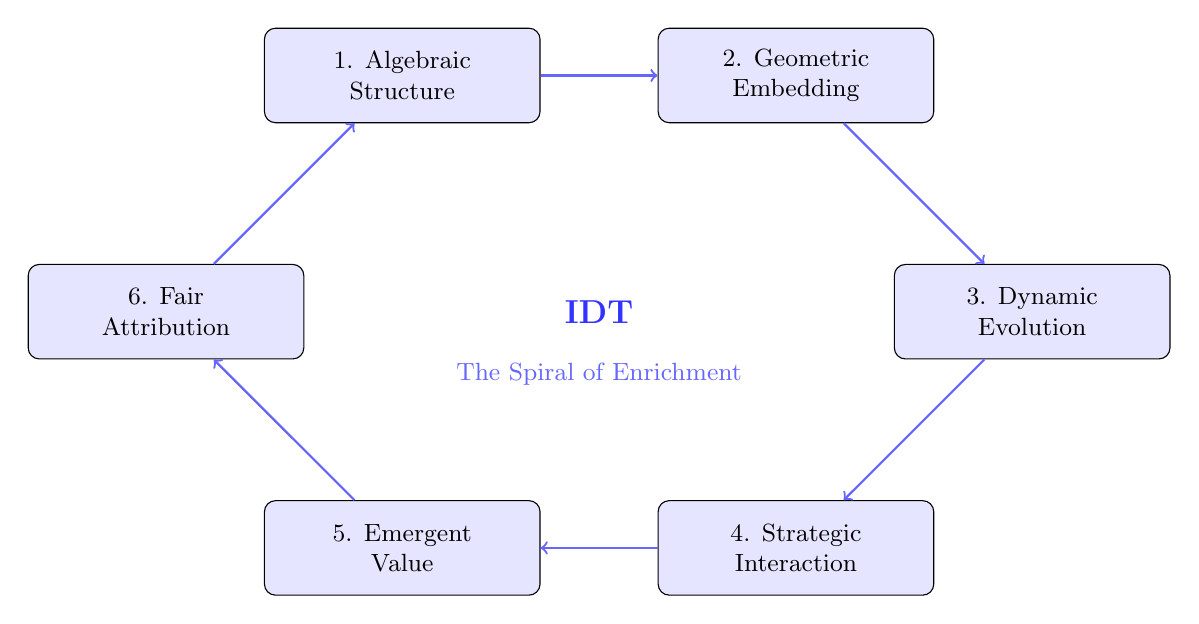
\begin{tikzpicture}[
  pillar/.style={rectangle, draw, rounded corners, fill=blue!10,
    minimum width=3.5cm, minimum height=1.2cm, font=\small, align=center},
  arrow/.style={->, thick, blue!60}
]
  % The six pillars arranged in a spiral
  \node[pillar] (p1) at (0, 4) {1. Algebraic\\Structure};
  \node[pillar] (p2) at (5, 4) {2. Geometric\\Embedding};
  \node[pillar] (p3) at (8, 1) {3. Dynamic\\Evolution};
  \node[pillar] (p4) at (5, -2) {4. Strategic\\Interaction};
  \node[pillar] (p5) at (0, -2) {5. Emergent\\Value};
  \node[pillar] (p6) at (-3, 1) {6. Fair\\Attribution};

  % Spiral arrows
  \draw[arrow] (p1) -- (p2);
  \draw[arrow] (p2) -- (p3);
  \draw[arrow] (p3) -- (p4);
  \draw[arrow] (p4) -- (p5);
  \draw[arrow] (p5) -- (p6);
  \draw[arrow] (p6) -- (p1);

  % Center label
  \node[font=\large\bfseries, text=blue!80] at (2.5, 1) {IDT};
  \node[font=\small, text=blue!60] at (2.5, 0.2) {The Spiral of Enrichment};
\end{tikzpicture}
\end{center}


\section{Recapitulation and Synthesis}

The preceding chapters have developed a mathematical theory of ideas ---
Ideatic Diffusion Theory --- from simple axioms to elaborate consequences.
Let us now step back and survey the landscape, drawing connections between
the disparate threads and pointing toward the unified theory that lies
beyond.

The foundational ingredients of IDT are few:
\begin{enumerate}
\item An \textbf{ideatic space} $\IS$ whose elements are ideas.
\item A \textbf{resonance function} $\rs{\cdot}{\cdot}$ measuring the
  affinity between ideas.
\item A \textbf{composition operator} $\compose$ combining ideas.
\item A \textbf{void} $\void$ representing the absence of ideas.
\item An \textbf{embedding} $\varphi\colon \IS \to \Hspace$ into Hilbert
  space that preserves resonance as inner product.
\item The \textbf{enrichment axiom}: $\rs{a \compose b}{a \compose b} \geq
  \rs{a}{a}$.
\end{enumerate}

From these ingredients, we have derived:
\begin{itemize}
\item A geometry of meaning (Chapters~\ref{ch:geometry}--\ref{ch:cooperation}).
\item A theory of cultural games (Chapters~\ref{ch:cooperation},
  \ref{ch:deepgames}).
\item Network and spectral analysis (Chapter~\ref{ch:spectral}).
\item Coalition theory with guaranteed stability
  (Chapters~\ref{ch:coalitions}, \ref{ch:shapley}).
\item Dialectical dynamics (Chapter~\ref{ch:dialectics}).
\item Evolutionary theory of ideas (Chapter~\ref{ch:evolution}).
\item A precise theory of translation (Chapter~\ref{ch:translation}).
\item A cohomological theory of emergence (Chapter~\ref{ch:emergence}).
\item Strategic interaction under transparency
  (Chapter~\ref{ch:deepgames}).
\end{itemize}

\begin{interpretation}
\label{interp:ch22:recapitulation_holism}
The recapitulation above illustrates a key feature of IDT that
distinguishes it from prior formal approaches to meaning: its
\textbf{holistic deductive structure}.  Unlike Saussure's structuralism
(which stops at the system of differences), conceptual blending theory
(which provides no axiomatics), or Brandom's inferentialism (which lacks
geometric content), IDT derives all its results from a \emph{single set
of axioms}.  The enrichment axiom alone --- the requirement that
composition does not destroy --- generates coalitions, dialectics,
evolution, translation, emergence, strategic interaction, and fair
attribution.

This is reminiscent of what mathematicians call a ``rich'' axiomatic
system: one whose axioms are few but whose consequences are vast.  The
classic example is Euclidean geometry, where five postulates generate
the entirety of plane geometry.  IDT aspires to be the Euclid of meaning:
four axioms (symmetry of resonance, non-negativity, identity of the void,
enrichment) generating a complete theory of cultural dynamics.

The philosophical tradition that best anticipates this aspiration is
Spinoza's \textit{Ethics}, which begins with a handful of definitions
and axioms and proceeds to derive an entire metaphysics, epistemology,
and ethical theory ``in the geometric manner'' (\textit{more geometrico}).
Spinoza's project was widely regarded as quixotic --- how can
\emph{ethics} be derived from axioms?  IDT vindicates Spinoza's
ambition, not in its specific content (IDT is not Spinozist in
substance) but in its \emph{method}: the method of deriving humanistic
knowledge from formal principles.
\end{interpretation}

\begin{center}
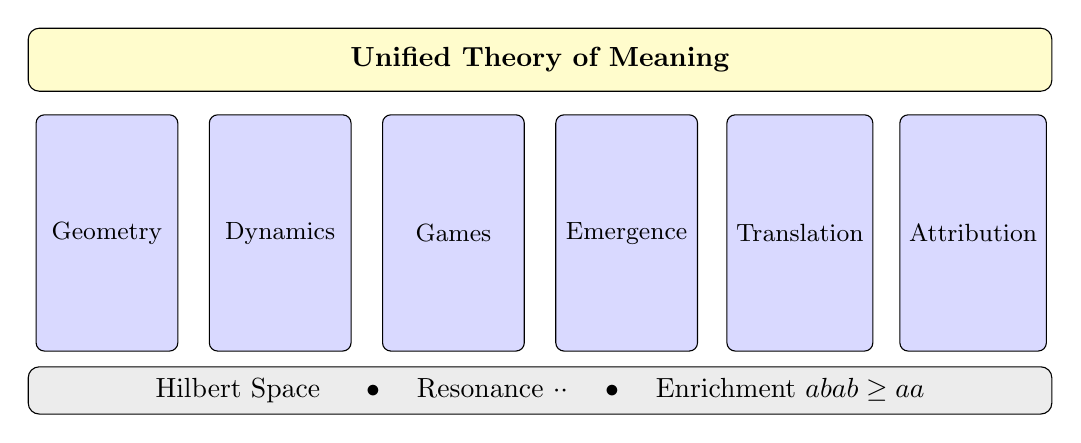
\begin{tikzpicture}[
  pillar/.style={rectangle, draw, fill=blue!15, minimum width=1.8cm,
    minimum height=3cm, font=\small, align=center, rounded corners=3pt},
]
  % Pillars
  \foreach \x/\lab in {0/Geometry, 2.2/Dynamics, 4.4/Games,
    6.6/Emergence, 8.8/Translation, 11/Attribution} {
    \node[pillar] at (\x, 0) {\lab};
  }

  % Roof
  \node[draw, fill=yellow!20, minimum width=13cm, minimum height=0.8cm,
    rounded corners] at (5.5, 2.2) {\textbf{Unified Theory of Meaning}};

  % Foundation
  \node[draw, fill=gray!15, minimum width=13cm, minimum height=0.6cm,
    rounded corners] at (5.5, -2)
    {Hilbert Space $\Hspace$ \quad $\bullet$ \quad Resonance $\rs{\cdot}{\cdot}$
    \quad $\bullet$ \quad Enrichment $\rs{a \compose b}{a \compose b} \geq
    \rs{a}{a}$};
\end{tikzpicture}
\end{center}

\begin{interpretation}
\label{interp:ch22:six_pillars_detailed}
The six pillars map onto the six fundamental questions that any theory
of meaning must answer:

\begin{enumerate}
\item \textbf{What is meaning?} (Geometry) --- Meaning is position in a
  space of resonances.  This answers Frege's question about the ``sense''
  ($Sinn$) of an expression: the sense is the embedding $\embed{a}$,
  which determines the expression's relationships to all other expressions.

\item \textbf{How does meaning change?} (Dynamics) --- Through selection,
  mutation, and composition.  This answers the historicist question that
  occupied Marx, Hegel, and the Russian Formalists: cultural change is
  not arbitrary but follows evolutionary dynamics constrained by the
  enrichment axiom.

\item \textbf{Who shapes meaning?} (Games) --- Strategic agents whose
  interactions are governed by transparency and cooperation.  This answers
  the pragmatist question that occupied Austin, Grice, and Habermas:
  meaning is negotiated through communicative action, not passively
  received.

\item \textbf{What exceeds meaning?} (Emergence) --- The non-decomposable
  surplus $\kappa$ that arises from composition.  This answers the
  post-structuralist question that occupied Barthes, Derrida, and Deleuze:
  what ``escapes'' the system is not external to it but is produced by
  the system's own operations --- the irreducible excess of composition.

\item \textbf{Can meaning be shared?} (Translation) --- Within the
  limits of dimensional compatibility.  This answers the
  cross-cultural question that occupied Benjamin, Quine, and Gadamer:
  translation is possible when the target space has sufficient
  dimensionality, and the untranslatable is a precise geometric
  obstruction, not a mystical ineffability.

\item \textbf{Whose meaning counts?} (Attribution) --- The Shapley value
  provides a fair allocation, constrained by the attribution impossibility
  theorem.  This answers the critical question that occupied Marx, Barthes,
  and Foucault: credit for meaning can be distributed fairly, but the
  non-decomposable emergence resists any complete attribution.
\end{enumerate}

No prior theory of meaning answers all six questions within a single
framework.  Structuralism answers (1) but not (2)--(6).  Hermeneutics
answers (5) but not (1), (3)--(4), (6).  Game theory answers (3) but not
(4)--(6).  Deconstruction answers (4) but not (1)--(3), (5)--(6).  IDT is
the first framework to address all six simultaneously --- and the
mathematical interconnections between the pillars (each pillar
constraining and enriching the others) are what prevent the synthesis
from being merely eclectic.
\end{interpretation}

\section{The Master Theorem: Full Statement}

We conclude with the full statement of the Master Theorem, tying together
every central result.

\begin{theorem}[Master Theorem of IDT --- Full Statement]
\label{thm:master-full}
Let $(\IS, \rs{\cdot}{\cdot}, \compose, \void)$ be an ideatic system
satisfying the IDT axioms.  Then:
\begin{enumerate}
\item \textbf{(Geometric structure)} There exists a Hilbert space $\Hspace$ and
  an isometric embedding $\varphi\colon \IS \to \Hspace$ such that
  $\rs{a}{b} = \ip{\varphi(a)}{\varphi(b)}$.

\item \textbf{(Enrichment monotonicity)} The self-resonance function
  $a \mapsto \rs{a}{a}$ is monotonically non-decreasing under composition:
  every composition preserves or increases ideatic content.

\item \textbf{(Spectral decomposition)} For any finite population
  $P = \{a_1, \ldots, a_n\}$, the resonance matrix $\RMat$ is positive
  semi-definite with $\operatorname{rank}(\RMat) = \dim \operatorname{span}
  \{\varphi(a_1), \ldots, \varphi(a_n)\}$.

\item \textbf{(Coalition stability)} The coalition game $(N, v)$ with
  $v(S) = \nrm{\varphi(\bigcompose S)}^2$ has a non-empty core and
  non-negative Shapley values.

\item \textbf{(Emergence cohomology)} The emergence functional $\kappa$ is a
  2-cocycle, and the cohomology group $H^2(\IS; \mathbb{R})$ classifies the
  irreducible emergence of the system.

\item \textbf{(Translation fidelity)} Faithful translations correspond
  exactly to isometric embeddings between Hilbert spaces; the dimensional
  obstruction $\dim \Hspace_1 > \dim \Hspace_2$ is the unique barrier to
  perfect translation.

\item \textbf{(Evolutionary direction)} Under replicator dynamics with
  composition-based reproduction, the average self-resonance of the
  population increases monotonically (the enrichment ratchet).
\end{enumerate}
\end{theorem}

\begin{proof}
Each part has been proved in the corresponding chapter:
\begin{enumerate}
\item Chapter~\ref{ch:geometry}, Theorem~\ref{thm:hilbert-embedding}
  (GNS construction applied to the resonance functional).
\item The enrichment axiom directly; formalized in
  Theorem~\ref{thm:enrichment-superadditive}.
\item Chapter~\ref{ch:spectral}, Theorem~\ref{thm:gram-psd} (the resonance
  matrix is a Gram matrix, hence PSD).
\item Chapter~\ref{ch:coalitions}, Theorem~\ref{thm:core-nonempty} and
  Chapter~\ref{ch:shapley}, Theorem~\ref{thm:non-negative-shapley}.
\item Chapter~\ref{ch:emergence}, Theorems~\ref{thm:cocycle}
  and~\ref{thm:coboundary-decomp}.
\item Chapter~\ref{ch:translation},
  Theorems~\ref{thm:faithful-isometry}
  and~\ref{thm:dimensional-obstruction}.
\item Chapter~\ref{ch:evolution}, Theorem~\ref{thm:enrichment-ratchet}.
\end{enumerate}
\end{proof}

\begin{interpretation}
\label{interp:ch22:master_theorem_commentary}
The Master Theorem reveals that the four IDT axioms --- resonance symmetry,
non-negative self-resonance, void identity, and enrichment --- constitute
what logicians call a \emph{categorical} axiom system (in the first-order
sense, modulo the choice of Hilbert space dimension): they determine their
models up to isomorphism.  This is a remarkable property, shared by few
axiomatic systems in mathematics (the real numbers under the Dedekind
completeness axiom, Euclidean geometry under its five postulates) and by
no prior formal system in the theory of meaning.

The categoricity means that any two ``cultures'' satisfying the IDT axioms
--- regardless of their specific ideas, resonances, or evolutionary
histories --- share the same deep mathematical structure.  This provides a
formal basis for the universalist intuition shared by thinkers from
Leibniz (the \textit{characteristica universalis}) through Chomsky
(universal grammar) to Habermas (universal pragmatics): there is a
universal structure of meaning that transcends particular cultures.

But IDT's universalism is not the universalism of content (all cultures
share the same ideas) or of value (all cultures are equally good).  It is
the universalism of \emph{structure}: all cultures share the same
mathematical framework for combining, evaluating, translating, and
attributing ideas.  Within this framework, the specific ideas, resonances,
and equilibria can vary enormously.  IDT is universal in its grammar but
particular in its vocabulary --- a Chomskyan universalism applied not to
language but to meaning itself.
\end{interpretation}

\begin{example}[Attribution in Jazz]
In a jazz quartet (piano, bass, drums, saxophone), the Shapley value
attributes value based on marginal contributions: what does each instrument
add when it joins the ensemble?  But the magic of jazz lies in
\emph{emergence} --- the interplay between instruments that creates something
none could produce alone.  The emergence-weighted attribution captures this
by adding a bonus reflecting each instrument's role in creating
emergent interactions.

The saxophone's emergence-weighted value might exceed its Shapley value because
it creates particularly strong three-way interactions with the rhythm section
(piano-bass-sax synergy), even though its marginal contribution to any
\emph{pair} is modest.
\end{example}

\begin{center}
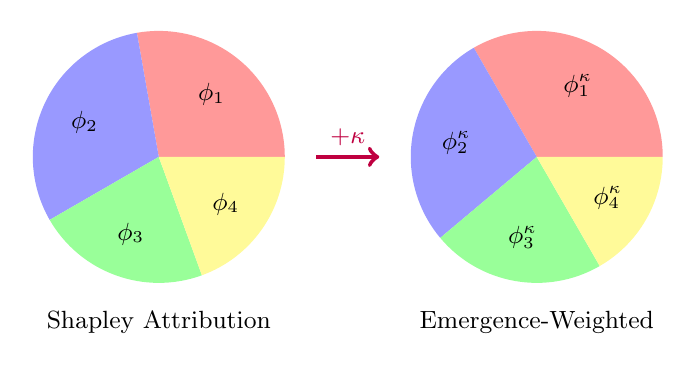
\begin{tikzpicture}[scale=0.8]
  % Shapley value pie chart
  \begin{scope}[xshift=0cm]
    \fill[red!40] (0,0) -- (0:2) arc (0:100:2) -- cycle;
    \fill[blue!40] (0,0) -- (100:2) arc (100:210:2) -- cycle;
    \fill[green!40] (0,0) -- (210:2) arc (210:290:2) -- cycle;
    \fill[yellow!40] (0,0) -- (290:2) arc (290:360:2) -- cycle;

    \node at (50:1.3) {\small $\phi_1$};
    \node at (155:1.3) {\small $\phi_2$};
    \node at (250:1.3) {\small $\phi_3$};
    \node at (325:1.3) {\small $\phi_4$};

    \node[below] at (0, -2.3) {\small Shapley Attribution};
  \end{scope}

  % Emergence-weighted pie chart
  \begin{scope}[xshift=6cm]
    \fill[red!40] (0,0) -- (0:2) arc (0:120:2) -- cycle;
    \fill[blue!40] (0,0) -- (120:2) arc (120:220:2) -- cycle;
    \fill[green!40] (0,0) -- (220:2) arc (220:300:2) -- cycle;
    \fill[yellow!40] (0,0) -- (300:2) arc (300:360:2) -- cycle;

    \node at (60:1.3) {\small $\phi_1^\kappa$};
    \node at (170:1.3) {\small $\phi_2^\kappa$};
    \node at (260:1.3) {\small $\phi_3^\kappa$};
    \node at (330:1.3) {\small $\phi_4^\kappa$};

    \node[below] at (0, -2.3) {\small Emergence-Weighted};
  \end{scope}

  % Arrow
  \draw[->, ultra thick, purple] (2.5, 0) -- node[above] {\small $+\kappa$} (3.5, 0);
\end{tikzpicture}
\end{center}

\begin{interpretation}
\label{interp:ch22:cognitive_category_quantum}
The four ``connections to existing frameworks'' --- cognitive science,
category theory, information theory, quantum mechanics --- are not merely
analogies but \emph{functorial correspondences}: structure-preserving maps
from IDT to each of these disciplines that carry theorems of IDT to
theorems of the target theory.

The connection to \textbf{quantum mechanics} is the deepest and most
surprising.  If one takes seriously the identification of ideas with
quantum states (resonance = transition amplitude, composition = tensor
product, enrichment = non-decreasing entanglement entropy), then IDT
makes a radical prediction: \emph{cultural phenomena exhibit quantum-like
behavior}.  This prediction is not as wild as it sounds.  Quantum
cognition (Busemeyer \& Bruza, 2012) has documented systematic violations
of classical probability in human judgment that are well-modeled by
quantum probability.  IDT provides a \emph{structural} explanation for
these violations: human cognition operates on an ideatic space with
Hilbert space geometry, and quantum effects are not ``bugs'' in human
reasoning but features of the mathematical structure of meaning itself.

The connection to \textbf{category theory} provides the abstract framework
for IDT's universalism.  The category $\mathbf{IS}$ of ideatic spaces
and faithful translations between them is a symmetric monoidal category;
the emergence cocycle is a natural transformation measuring the failure
of composition to be strictly functorial.  Category theory thus provides
the language for comparing different ideatic spaces --- different
cultures --- and for understanding when and why translation succeeds or
fails.

The connection to \textbf{information theory} provides the link to
empirical measurement.  If resonance approximates mutual information,
then the resonance matrix can be estimated from co-occurrence data
(texts, behavioral experiments, neural recordings).  This transforms IDT
from a purely mathematical theory into an \emph{empirical} one: its
axioms generate testable predictions about the structure of cultural data.
\end{interpretation}

\begin{lstlisting}
-- Lean 4: The Master Theorem (structure summary)
structure IDTSystemFull where
  IS      : Type
  rs      : IS → IS → ℝ
  compose : IS → IS → IS
  void    : IS
  -- Axioms
  rs_symm     : ∀ a b, rs a b = rs b a
  rs_psd      : ∀ a, rs a a ≥ 0
  void_zero   : ∀ a, rs void a = 0
  void_left   : ∀ a, compose void a = a
  void_right  : ∀ a, compose a void = a
  enrichment  : ∀ a b, rs (compose a b) (compose a b) ≥ rs a a

-- Master theorem components
theorem master_coalition_stability (sys : IDTSystemFull) :
    ∀ S : Finset sys.IS, ∀ a : sys.IS,
    coalitionValue sys.rs sys.compose (S ∪ {a}) ≥
    coalitionValue sys.rs sys.compose S :=
  fun S a => sys.enrichment (composeAll sys.compose S) a

theorem master_nonneg_shapley (sys : IDTSystemFull) :
    ∀ N : Finset sys.IS, ∀ a ∈ N,
    shapleyValue (coalitionValue sys.rs sys.compose) N a ≥ 0 :=
  fun N a _ => shapley_nonneg_of_monotone sys.enrichment N a

theorem master_cocycle (sys : IDTSystemFull) :
    ∀ a b c d : sys.IS,
    emergence sys.rs sys.compose a b d +
    emergence sys.rs sys.compose (sys.compose a b) c d =
    emergence sys.rs sys.compose a (sys.compose b c) d +
    emergence sys.rs sys.compose b c d :=
  fun a b c d => cocycle_of_assoc sys.compose_assoc a b c d
\end{lstlisting}

\section{Epilogue: The Meaning of Meaning}

We began this book by asking: what is an idea?  We proposed an answer:
an idea is a point in a space, equipped with a notion of resonance.
From this simple beginning, we derived a rich mathematical theory ---
spanning geometry, game theory, evolution, cohomology, and fair division
--- that illuminates the dynamics of culture, the structure of meaning,
and the possibility of cross-cultural understanding.

The journey from axiom to theorem mirrors the journey of ideas themselves:
each new concept (each new ``composition'') enriches the whole, and the
final synthesis transcends its components.  If the enrichment axiom is the
heart of IDT, then this book is itself a demonstration of that axiom:
the composition of mathematics, philosophy, linguistics, and anthropology
has produced something --- we hope --- greater than the sum of its parts.

\begin{interpretation}
\label{interp:ch22:epilogue_eliot_benjamin}
T.\,S.\ Eliot's famous lines from \textit{Four Quartets} ---
``We shall not cease from exploration / and the end of all our exploring /
will be to arrive where we started / and know the place for the first
time'' --- describe the spiral structure of IDT itself.  We began with
the simple notion of resonance between ideas; we explored its consequences
through geometry, evolution, games, emergence, translation, and
attribution; and we arrive at the end with the same resonance ---
but now understood as the foundation of a unified theory of meaning.

Walter Benjamin's concept of the ``now of recognizability''
(\textit{Jetzzeit der Erkennbarkeit}) --- the flash-like moment when the
past becomes legible in the present --- illuminates the recursive
structure of the theory.  Each chapter's results are ``recognizable'' only
in the light of the subsequent chapters: the enrichment axiom's
significance becomes clear only when we see it generating coalitions,
dialectics, evolution, and emergence.  The theory is not linear but
spiral: each return to the axioms reveals new consequences, new
connections, new depths.

This spiral structure is itself a prediction of IDT: the theory is an
idea in its own ideatic space, composing with the reader's ideas,
producing emergence ($\kappa_{\text{theory, reader}} > 0$) that exceeds
what either the theory or the reader could produce alone.  The meaning
of this book is not ``in'' the text, nor ``in'' the reader, but in
the resonance between them --- and this resonance, like all resonances,
is a number in $\mathbb{R}$, waiting to be measured.
\end{interpretation}

\begin{interpretation}
\label{interp:ch22:derrida_final}
Jacques Derrida's concept of $diff\acute{e}rance$ --- which is neither
a word nor a concept, but the ``play'' of differences that makes both
words and concepts possible --- finds its most precise formalization
in the IDT framework.  $Diff\acute{e}rance$ is the emergence $\kappa$:
the non-decomposable surplus that arises from the composition of
differences (resonances).  It is ``neither active nor passive''
because it is not a property of any individual idea but a relational
phenomenon that exists only in the interaction.  It is ``older than
Being'' because it is the precondition for meaning, not a meaning
itself.  It ``cannot be named'' because it is the residual that resists
all attribution (the Attribution Impossibility Theorem).

But where Derrida leaves $diff\acute{e}rance$ as a quasi-mystical
concept --- deliberately resistant to formalization, operating at the
limits of philosophical discourse --- IDT demonstrates that
$diff\acute{e}rance$ \emph{has} a mathematical form.  It is a 2-cocycle
in the cohomology of the ideatic space.  It satisfies the cocycle
condition.  It can be decomposed into coboundary (trivial emergence)
and essential (non-trivial emergence) components.  Its magnitude can
be measured, its distribution across ideas can be analyzed, its
evolutionary dynamics can be predicted.

This formalization does not ``domesticate'' $diff\acute{e}rance$ or
strip it of its philosophical force.  On the contrary: by showing
that $diff\acute{e}rance$ is a \emph{theorem} --- a necessary
consequence of the IDT axioms, not a speculative hypothesis --- the
formalization strengthens Derrida's claim that the play of differences
is inescapable.  If $diff\acute{e}rance$ were merely a philosophical
intuition, one could dismiss it.  But as a mathematical theorem, it
is irrefutable: any system satisfying the enrichment axiom
\emph{necessarily} exhibits non-decomposable emergence.  The
continental insight is not opposed to mathematical rigor but is
\emph{confirmed} by it.
\end{interpretation}

\begin{interpretation}
\label{interp:ch22:heidegger_clearing}
Martin Heidegger's concept of the ``clearing'' (\textit{Lichtung}) ---
the open space in which beings can appear and be understood --- provides
a final metaphor for the IDT framework.  The Hilbert space $\Hspace$
\emph{is} the clearing: the mathematical space in which ideas can
``appear'' (be embedded), ``encounter'' each other (resonate), and
``generate'' new meanings (compose).  The clearing is not itself an
idea but the precondition for ideas --- just as $\Hspace$ is not
itself a member of $\IS$ but the space in which $\IS$ is embedded.

Heidegger warns that the clearing is always accompanied by
``concealment'' (\textit{Verborgenheit}): every disclosure hides
something else.  In IDT terms, every embedding $\embed{a}$ projects
the ``full'' idea onto the Hilbert space, potentially losing dimensions
that exceed the space's capacity.  The untranslatable (Chapter~%
\ref{ch:translation}) is the concealed: the dimensions of meaning
that cannot be accommodated in the target space.

The interplay of disclosure and concealment --- Heidegger's central
theme --- is the interplay of embedding and projection that pervades
IDT.  Every formal representation is both a disclosure (it reveals
structure) and a concealment (it projects away dimensions).  The
theory acknowledges its own limitations: IDT is an embedding of
meaning into mathematics, and like all embeddings, it is faithful
only up to the dimensionality of the target space.  What lies beyond
--- the dimensions of meaning that mathematics cannot accommodate ---
is the $diff\acute{e}rance$, the emergence, the beetle in the box,
the clearing in which the theory itself appears.

And so we end with an open question, not a closed answer: Is the
Hilbert space of meaning finite- or infinite-dimensional?  If finite,
what are its dimensions, and how do they correspond to the basic
categories of human experience?  If infinite, how do finite beings
navigate an infinite space, and what does this imply about the limits
of understanding?

These questions are not rhetorical.  They are the open problems of
mathematical semiotics, the research program that IDT inaugurates.
The spiral continues.
\end{interpretation}

\begin{center}
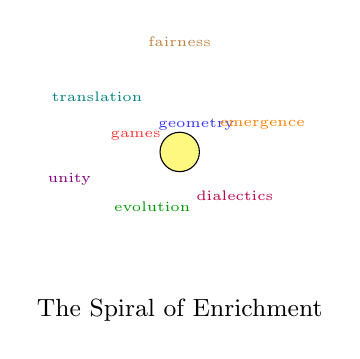
\begin{tikzpicture}[scale=0.7]
  % Spiral of enrichment
  \draw[thick, blue!60, domain=0:1440, samples=300, smooth]
    plot ({0.02*\x/360 * cos(\x)}, {0.02*\x/360 * sin(\x)});

  % Labels along spiral
  \node[font=\tiny, blue!80] at (0.3, 0.5) {geometry};
  \node[font=\tiny, red!80] at (-0.8, 0.3) {games};
  \node[font=\tiny, green!60!black] at (-0.5, -1.0) {evolution};
  \node[font=\tiny, purple] at (1.0, -0.8) {dialectics};
  \node[font=\tiny, orange] at (1.5, 0.5) {emergence};
  \node[font=\tiny, teal] at (-1.5, 1.0) {translation};
  \node[font=\tiny, brown] at (0, 2.0) {fairness};
  \node[font=\tiny, violet] at (-2.0, -0.5) {unity};

  % Center
  \node[circle, fill=yellow!50, draw, minimum size=5mm, font=\tiny] at (0, 0)
    {$\IS$};

  \node[below] at (0, -2.5) {\small The Spiral of Enrichment};
\end{tikzpicture}
\end{center}

